% !TeX root = Dyplom.tex
% !TeX root = Dyplom.tex
\documentclass[a4paper,onecolumn,oneside,12pt,extrafontsizes]{memoir}

%    Do tego wystarczy posłużyć się poniższymi komendami (zamiast documentclass z pierwszej linijki):
%   \documentclass[a4paper,onecolumn,twoside,10pt]{memoir} 
%   \renewcommand{\normalsize}{\fontsize{8pt}{10pt}\selectfont}
\usepackage[utf8]{inputenc} % Proszę użyć zamiast powyższego, jeśli kodowanie edytowanych plików to UTF8
\usepackage[T1]{fontenc}
\usepackage[english,polish]{babel} % Tutaj ważna jest kolejność atrybutów (dla pracy po polsku polish powinno być na końcu)
%\DisemulatePackage{setspace}
\usepackage{setspace}
\usepackage{color,calc}
%\usepackage{soul} % pakiet z komendami do podkreślania, przekreślania, podświetlania tekstu (raczej niepotrzebny)
\usepackage{ebgaramond} % pakiet z czcionkami garamond, potrzebny tylko do strony tytułowej, musi wystąpić przed pakietem tgtermes
\usepackage{float}
\usepackage{etoolbox}

\usepackage{subcaption}
%% Aby uzyskać polskie literki w pdfie (a nie zlepki) korzystamy z pakietu czcionek tgterms. 
%% W pakiecie tym są zdefiniowane klony czcionek Times o kształtach: normalny, pogrubiony, italic, italic pogrubiony.
%% W pakiecie tym brakuje czcionki o kształcie: slanted (podobny do italic). 
%% Jeśli w dokumencie gdzieś zostanie zastosowana czcionka slanted (np. po użyciu komendy \textsl{}), to
%% latex dokona podstawienia na czcionkę standardową i zgłosi to w ostrzeżeniu (warningu).
%% Ponadto tgtermes to czcionka do tekstu. Wszelkie matematyczne wzory będą sformatowane domyślną czcionką do wzorów.
%% Jeśli wzory mają być sformatowane z wykorzystaniem innych czcionek, trzeba to jawnie zadeklarować.

\usepackage{tgtermes}   
\renewcommand*\ttdefault{txtt}


%%%%%%%%%%%%%%%%%%%%%%%%%%%%%%%%%%%%%%%%%%%%%%%%%%%%%%%%%%%%%%%%%%%%%%%%%%%%%%%%
%% Ustawienia odpowiedzialne za sposób łamania dokumentu
%% i ułożenie elementów pływających
%%%%%%%%%%%%%%%%%%%%%%%%%%%%%%%%%%%%%%%%%%%%%%%%%%%%%%%%%%%%%%%%%%%%%%%%%%%%%%%%
\clubpenalty=10000      % kara za sierotki
\widowpenalty=10000     % nie pozostawiaj wdów
\righthyphenmin=3			  % dziel minimum 3 litery

\renewcommand{\topfraction}{0.95}
\renewcommand{\bottomfraction}{0.95}
\renewcommand{\textfraction}{0.05}
\renewcommand{\floatpagefraction}{0.35}

%%%%%%%%%%%%%%%%%%%%%%%%%%%%%%%%%%%%%%%%%%%%%%%%%%%%%%%%%%%%%%%%%%%%%%%%%%%%%%%%
%%  Ustawienia rozmiarów: tekstu, nagłówka i stopki, marginesów
%%  dla dokumentów klasy memoir 
%%%%%%%%%%%%%%%%%%%%%%%%%%%%%%%%%%%%%%%%%%%%%%%%%%%%%%%%%%%%%%%%%%%%%%%%%%%%%%%%
\setlength{\headsep}{3mm} 
\setlength{\headheight}{13.6pt} % wartość baselineskip dla czcionki 11pt tj. \small wynosi 13.6pt
\setlength{\footskip}{\headsep+\headheight}
\setlength{\uppermargin}{\headheight+\headsep+1cm}
\setlength{\textheight}{\paperheight-\uppermargin-\footskip-1.5cm}
\setlength{\textwidth}{\paperwidth-5cm}
\setlength{\spinemargin}{2.5cm}
\setlength{\foremargin}{2.5cm}
\setlength{\marginparsep}{2mm}
\setlength{\marginparwidth}{2.3mm}
\checkandfixthelayout[fixed] % konieczne, aby się dobrze wszystko poustawiało
%%%%%%%%%%%%%%%%%%%%%%%%%%%%%%%%%%%%%%%%%%%%%%%%%%%%%%%%%%%%%%%%%%%%%%%%%%%%%%%%
%%  Ustawienia odległości linii, wcięć, odstępów
%%%%%%%%%%%%%%%%%%%%%%%%%%%%%%%%%%%%%%%%%%%%%%%%%%%%%%%%%%%%%%%%%%%%%%%%%%%%%%%%
\linespread{1}
%\linespread{1.241}
\setlength{\parindent}{14.5pt}


\usepackage{multicol} % pakiet umożliwiający stworzenie wielokolumnowego tekstu
%%%%%%%%%%%%%%%%%%%%%%%%%%%%%%%%%%%%%%%%%%%%%%%%%%%%%%%%%%%%%%%%%%%%%%%%%%%%%%%%
%% Pakiety do formatowania tabel
%%%%%%%%%%%%%%%%%%%%%%%%%%%%%%%%%%%%%%%%%%%%%%%%%%%%%%%%%%%%%%%%%%%%%%%%%%%%%%%%
\usepackage{tabularx}

%%%%%%%%%%%%%%%%%%%%%%%%%%%%%%%%%%%%%%%%%%%%%%%%%%%%%%%%%%%%%%%%%%%%%%%%%%%%%%%%
%% Pakiet do wstawiania fragmentów kodu
%%%%%%%%%%%%%%%%%%%%%%%%%%%%%%%%%%%%%%%%%%%%%%%%%%%%%%%%%%%%%%%%%%%%%%%%%%%%%%%%
\usepackage{listings} 
\usepackage{listingsutf8}
\usepackage[linesnumbered,ruled,vlined]{algorithm2e}
% Zmiana "Algorithm" na "Algorytm"
\renewcommand{\algorithmcfname}{Algorytm}
\usepackage{framed}
\usepackage{xpatch}
\makeatletter
\xpatchcmd\l@lstlisting{1.5em}{0em}{}{}
\makeatother
% Pakiet dostarcza otoczenia lstlisting. Jest ono wysoce konfigurowalne. 
% Konfigurować można indywidualnie każdy z listingów lub globalnie, w poleceniu \lstset{}.

% Zalecane jest, by kod źródłowy był wyprowadzany z użyciem czcionki maszynowej \ttfamily
% Ponieważ kod źródłowy, nawet po obcięciu do interesujących fragmentów, bywa obszerny, należy zmniejszyć czcionkę.
% Zalecane jest \small (dla krótkich fragmentów) oraz \footnotesize (dla dłuższych fragmentów).

% Ponadto podczas konfiguracji można zadeklarować sposób numerowania linii. Numerowanie linii zalecane jest jednak 
% tylko w przypadkach, gdy w redagowanym tekście znajdują się jakieś odwołania do konkretnych linii.
% Jeśli takich odwołań nie ma, numerowanie linii jest zbędne. Proszę wtedy go nie stosować.
% Przy włączaniu numerowania linii należy zwrócić uwagę na to, gdzie pojawią się te numery.
% Bez zmiany dodatkowych parametrów pojawiają się one na marginesie strony (co jest niepożądane).

\lstset{
  basicstyle=\small\ttfamily, % lub basicstyle=\footnotesize\ttfamily
  inputencoding=utf8,
  %%columns=fullflexible,
	%%showstringspaces=false,
	%%showspaces=false,
  breaklines=true,
  postbreak=\mbox{\textcolor{red}{$\hookrightarrow$}\space}, 
  %%numbers=left,  % ta i poniższe linie dotyczą ustawienia numerowania i sposobu jego wyprowadzania
  %%firstnumber=1, 
  %%numberfirstline=true, 
	%%xleftmargin=17pt,
  %%framexleftmargin=17pt,
  %%framexrightmargin=5pt,
  %%framexbottommargin=4pt,
	belowskip=.5\baselineskip,
	literate={\_}{{\_\allowbreak}}1 % ta deklaracja przydaje się, jeśli na listingu mają być łamane nazwy zawierające podkreślniki
}
\lstset{literate=%-
{ą}{{\k{a}}}1 {ć}{{\'c}}1 {ę}{{\k{e}}}1 {ł}{{\l{}}}1 {ń}{{\'n}}1 {ó}{{\'o}}1 {ś}{{\'s}}1 {ż}{{\.z}}1 {ź}{{\'z}}1 {Ą}{{\k{A}}}1 {Ć}{{\'C}}1 {Ę}{{\k{E}}}1 {Ł}{{\L{}}}1 {Ń}{{\'N}}1 {Ó}{{\'O}}1 {Ś}{{\'S}}1 {Ż}{{\.Z}}1 {Ź}{{\'Z}}1 
    {Ö}{{\"O}}1
    {Ä}{{\"A}}1
    {Ü}{{\"U}}1
    {ß}{{\ss}}1
    {ü}{{\"u}}1
    {ä}{{\"a}}1
    {ö}{{\"o}}1
    {~}{{\textasciitilde}}1
    {—}{{{\textemdash} }}1
}%{\ \ }{{\ }}1}

%% Inne języki muszą być dodefiniowane. Poniżej podano przykłady definicji języków i styli.

\definecolor{lightgray}{rgb}{.9,.9,.9}
\definecolor{darkgray}{rgb}{.4,.4,.4}
\definecolor{purple}{rgb}{0.65, 0.12, 0.82}
\definecolor{javared}{rgb}{0.6,0,0} % for strings
\definecolor{javagreen}{rgb}{0.25,0.5,0.35} % comments
\definecolor{javapurple}{rgb}{0.5,0,0.35} % keywords
\definecolor{javadocblue}{rgb}{0.25,0.35,0.75} % javadoc


\lstdefinestyle{JavaStyle}{
basicstyle=\footnotesize\ttfamily,
keywordstyle=\color{javapurple}\bfseries,
stringstyle=\color{javared},
commentstyle=\color{javagreen},
morecomment=[s][\color{javadocblue}]{/**}{*/},
numbers=none,%left,
numberstyle=\tiny\color{black},
stepnumber=2,
numbersep=10pt,
tabsize=4,
showspaces=false,
showstringspaces=false,
captionpos=t
}

\definecolor{BackgroundRust}{RGB}{255,255,255}
\definecolor{GrayCodeBlock}{RGB}{241,241,241}
\definecolor{BlackText}{RGB}{110,107,94}
\definecolor{RedTypename}{RGB}{182,86,17}
\definecolor{GreenString}{RGB}{96,172,57}
\definecolor{PurpleKeyword}{RGB}{184,84,212}
\definecolor{GrayComment}{RGB}{170,170,170}
\definecolor{GoldDocumentation}{RGB}{180,165,45}
\lstdefinelanguage{rust}
{
    columns=fullflexible,
    keepspaces=true,
    frame=single,
    framesep=0pt,
    framerule=0pt,
    framexleftmargin=4pt,
    framexrightmargin=4pt,
    framextopmargin=5pt,
    framexbottommargin=3pt,
    xleftmargin=4pt,
    xrightmargin=4pt,
    backgroundcolor=\color{BackgroundRust},
    basicstyle=\ttfamily\color{BlackText},
    keywords={
        true,false,
        unsafe,async,await,move,
        use,pub,crate,super,self,mod,
        struct,enum,fn,const,static,let,mut,ref,type,impl,dyn,trait,where,as,
        break,continue,if,else,while,for,loop,match,return,yield,in
    },
    keywordstyle=\color{PurpleKeyword},
    ndkeywords={
        bool,u8,u16,u32,u64,u128,i8,i16,i32,i64,i128,char,str,
        Self,Option,Some,None,Result,Ok,Err,String,Box,Vec,Rc,Arc,Cell,RefCell,HashMap,BTreeMap,
        macro_rules
    },
    ndkeywordstyle=\color{RedTypename},
    comment=[l][\color{GrayComment}\slshape]{//},
    morecomment=[s][\color{GrayComment}\slshape]{/*}{*/},
    morecomment=[l][\color{GoldDocumentation}\slshape]{///},
    morecomment=[s][\color{GoldDocumentation}\slshape]{/*!}{*/},
    morecomment=[l][\color{GoldDocumentation}\slshape]{//!},
    morecomment=[s][\color{RedTypename}]{\#![}{]},
    morecomment=[s][\color{RedTypename}]{\#[}{]},
    stringstyle=\color{GreenString},
    string=[b]"
}

\definecolor{delim}{RGB}{20,105,176}
\definecolor{numb}{RGB}{106, 109, 32}
\definecolor{string}{rgb}{0.64,0.08,0.08}
\lstdefinelanguage{json}{
    showspaces=false,
    showtabs=false,
    breaklines=true,
    postbreak=\raisebox{0ex}[0ex][0ex]{\ensuremath{\color{GrayCodeBlock}\hookrightarrow\space}},
    breakatwhitespace=true,
    basicstyle=\ttfamily\small,
    upquote=true,
    morestring=[b]",
    stringstyle=\color{string},
    literate=
     *{0}{{{\color{numb}0}}}{1}
      {1}{{{\color{numb}1}}}{1}
      {2}{{{\color{numb}2}}}{1}
      {3}{{{\color{numb}3}}}{1}
      {4}{{{\color{numb}4}}}{1}
      {5}{{{\color{numb}5}}}{1}
      {6}{{{\color{numb}6}}}{1}
      {7}{{{\color{numb}7}}}{1}
      {8}{{{\color{numb}8}}}{1}
      {9}{{{\color{numb}9}}}{1}
      {\{}{{{\color{delim}{\{}}}}{1}
      {\}}{{{\color{delim}{\}}}}}{1}
      {[}{{{\color{delim}{[}}}}{1}
      {]}{{{\color{delim}{]}}}}{1},
}

\definecolor{pblue}{rgb}{0.13,0.13,1}
\definecolor{pgreen}{rgb}{0,0.5,0}
\definecolor{pred}{rgb}{0.9,0,0}
\definecolor{pgrey}{rgb}{0.46,0.45,0.48}
\definecolor{dark-grey}{rgb}{0.4,0.4,0.4}

% VS2017 C++ color scheme
\definecolor{clr-background}{RGB}{255,255,255}
\definecolor{clr-text}{RGB}{0,0,0}
\definecolor{clr-string}{RGB}{163,21,21}
\definecolor{clr-namespace}{RGB}{0,0,0}
\definecolor{clr-preprocessor}{RGB}{128,128,128}
\definecolor{clr-keyword}{RGB}{0,0,255}
\definecolor{clr-type}{RGB}{43,145,175}
\definecolor{clr-variable}{RGB}{0,0,0}
\definecolor{clr-constant}{RGB}{111,0,138} % macro color
\definecolor{clr-comment}{RGB}{0,128,0}

\lstdefinestyle{VS2017}{
	backgroundcolor=\color{clr-background},
	basicstyle=\color{clr-text}, % any text
	stringstyle=\color{clr-string},
	identifierstyle=\color{clr-variable}, % just about anything that isn't a directive, comment, string or known type
	commentstyle=\color{clr-comment},
	directivestyle=\color{clr-preprocessor}, % preprocessor commands
	% listings doesn't differentiate between types and keywords (e.g. int vs return)
	% use the user types color
	keywordstyle=\color{clr-type},
	keywordstyle={[2]\color{clr-constant}}, % you'll need to define these or use a custom language
	tabsize=4
}
% styl json
\newcommand\JSONnumbervaluestyle{\color{blue}}
\newcommand\JSONstringvaluestyle{\color{red}}

\newif\ifcolonfoundonthisline

\makeatletter

\lstdefinestyle{json-style}  
{
	showstringspaces    = false,
	keywords            = {false,true},
	alsoletter          = 0123456789.,
	morestring          = [s]{"}{"},
	stringstyle         = \ifcolonfoundonthisline\JSONstringvaluestyle\fi,
	MoreSelectCharTable =%
	\lst@DefSaveDef{`:}\colon@json{\processColon@json},
	basicstyle          = \footnotesize\ttfamily,
	keywordstyle        = \ttfamily\bfseries,
	numbers				= left, % zakomentować, jeśli numeracja linii jest niepotrzebna
	numberstyle={\footnotesize\ttfamily\color{dark-grey}},
	xleftmargin			= 2em % zakomentować, jeśli numeracja linii jest niepotrzebna
}

\newcommand\processColon@json{%
	\colon@json%
	\ifnum\lst@mode=\lst@Pmode%
	\global\colonfoundonthislinetrue%
	\fi
}

\lst@AddToHook{Output}{%
	\ifcolonfoundonthisline%
	\ifnum\lst@mode=\lst@Pmode%
	\def\lst@thestyle{\JSONnumbervaluestyle}%
	\fi
	\fi
	\lsthk@DetectKeywords% 
}

\lst@AddToHook{EOL}%
{\global\colonfoundonthislinefalse}

\makeatother
\usepackage{memlays}     % extra layout diagrams, zastosowane w szblonie do 'debuggowania', używa pakietu layouts
%\usepackage{layouts}
\usepackage{printlen} % pakiet do wyświetlania wartości zdefiniowanych długości, stosowany do 'debuggowania'
\usepackage{enumitem} % pakiet do numerowania 1.1 1.2 w sekcji enumrate
\uselengthunit{pt}
\makeatletter
\newcommand{\showFontSize}{\f@size pt} % makro wypisujące wielkość bieżącej czcionki
\makeatother
% do pokazania ramek można byłoby użyć:
%\usepackage{showframe} 

%%%%%%%%%%%%%%%%%%%%%%%%%%%%%%%%%%%%%%%%%%%%%%%%%%%%%%%%%%%%%%%%%%%%%%%%%%%%%%%%
%%  Formatowanie list wyliczeniowych, wypunktowań i własnych otoczeń
%%%%%%%%%%%%%%%%%%%%%%%%%%%%%%%%%%%%%%%%%%%%%%%%%%%%%%%%%%%%%%%%%%%%%%%%%%%%%%%%

% Domyślnie wypunktowania mają zadeklarowane znaki, które nie występują w tgtermes
% Aby latex nie podstawiał w ich miejsca znaków z czcionki standardowej można zrobić podstawienie:
%    \DeclareTextCommandDefault{\textbullet}{\ensuremath{\bullet}}
%    \DeclareTextCommandDefault{\textasteriskcentered}{\ensuremath{\ast}}
%    \DeclareTextCommandDefault{\textperiodcentered}{\ensuremath{\cdot}}
% Jednak jeszcze lepszym pomysłem jest zdefiniowanie otoczeń z wykorzystaniem enumitem
\usepackage{enumitem} % pakiet pozwalający zarządzać formatowaniem list wyliczeniowych
\setlist{noitemsep,topsep=4pt,parsep=0pt,partopsep=4pt,leftmargin=*} % zadeklarowane parametry pozwalają uzyskać 'zwartą' postać wypunktowania bądź wyliczenia
\setenumerate{labelindent=0pt,itemindent=0pt,leftmargin=!,label=\arabic*.} % można zmienić \arabic na \alph, jeśli wyliczenia mają być z literkami
\setlistdepth{4} % definiujemy głębokość zagnieżdżenia list wyliczeniowych do 4 poziomów
\setlist[itemize,1]{label=$\bullet$}  % definiujemy, jaki symbol ma być użyty w wyliczeniu na danym poziomie
\setlist[itemize,2]{label=\normalfont\bfseries\textendash}
\setlist[itemize,3]{label=$\ast$}
\setlist[itemize,4]{label=$\cdot$}
\renewlist{itemize}{itemize}{4}


\makeatletter
\renewenvironment{quote}{
	\begin{list}{}
	{
	\setlength{\leftmargin}{1em}
	\setlength{\topsep}{0pt}%
	\setlength{\partopsep}{0pt}%
	\setlength{\parskip}{0pt}%
	\setlength{\parsep}{0pt}%
	\setlength{\itemsep}{0pt}
	}
	}{
	\end{list}}
\makeatother

 \usepackage{datetime2} % INFO: pakiet potrzeby do uzyskania i sformatowania daty 
 \usepackage[pdftex,bookmarks,breaklinks,unicode]{hyperref}
 \usepackage[pdftex]{graphicx}
 \DeclareGraphicsExtensions{.pdf,.jpg,.mps,.png} % po zadeklarowaniu rozszerzeń można będzie wstawiać pliki z grafiką bez konieczności podawania tych rozszerzeń w ich nazwach
\pdfcompresslevel=9
\pdfoutput=1

% Dobrze przygotowany dokument pdf to taki, który zawiera metadane.
% Poniżej zadeklarowano pola metadanych, jakie będą włączone do dokumentu pdf.
% Można je zmodyfikować w zależności od potrzeb
\makeatletter
\pdftrailerid{} %Remove ID
\pdfsuppressptexinfo15 %Suppress PTEX.Fullbanner and info of imported PDFs
\makeatother
%\else             % jeśli kompilacja jest inna niż pdflatex
\usepackage{graphicx}
\DeclareGraphicsExtensions{.eps,.ps,.jpg,.mps,.png}
%\fi
\sloppy

% INFO: dodane by lepiej łamać urle 
\def\UrlBreaks{\do\/\do-\do_} 


%%%%%%%%%%%%%%%%%%%%%%%%%%%%%%%%%%%%%%%%%%%%%%%%%%%%%%%%%%%%%%%%%%%%%%%%%%%%%%%%
%%  Formatowanie dokumentu
%%%%%%%%%%%%%%%%%%%%%%%%%%%%%%%%%%%%%%%%%%%%%%%%%%%%%%%%%%%%%%%%%%%%%%%%%%%%%%%%
% INFO: Deklaracja głębokościu numeracji
\setcounter{secnumdepth}{2}
\setcounter{tocdepth}{2}
\setsecnumdepth{subsection} 
% INFO: Dodanie kropek po numerach sekcji
\makeatletter
\def\@seccntformat#1{\csname the#1\endcsname.\quad}
\def\numberline#1{\hb@xt@\@tempdima{#1\if&#1&\else.\fi\hfil}}
\makeatother
% INFO: Numeracja rozdziałów i separatory
\renewcommand{\chapternumberline}[1]{#1.\quad}
\renewcommand{\cftchapterdotsep}{\cftdotsep}

\makeatletter % odstępy w spisie pomiędzy rozdziałami
\renewcommand*{\insertchapterspace}{%
  \addtocontents{lof}{\protect\addvspace{3pt}}%
  \addtocontents{lot}{\protect\addvspace{3pt}}%
	\addtocontents{toc}{\protect\addvspace{3pt}} %
  \addtocontents{lol}{\protect\addvspace{3pt}}}
\makeatother 


\setlength{\cftbeforechapterskip}{0pt} % odstępy w spisie treści przed rozdziałem, działa w korelacji z:
\renewcommand{\aftertoctitle}{\afterchaptertitle\vspace{-4pt}} % 

% INFO: Czcionka do podpisów tabel, rysunków, listingów
\captionnamefont{\small}
\captiontitlefont{\small}

% INFO: Sformatowanie podpisu nad dwukolumnowym listingiem
\newcommand{\listingcaption}[1]
{%
\vspace*{\abovecaptionskip}\small 
\refstepcounter{lstlisting}\hfill%
Listing \thelstlisting: #1\hfill%\hfill%
\addcontentsline{lol}{lstlisting}{\protect\numberline{\thelstlisting}#1}
}%

% INFO: Pomocnicze marko do wyróżniania tekstu w języku angielskim
\newcommand{\eng}[1]{(ang.~\emph{#1})}
% IFNO: Pomocnicze makro do dołączania podpisów do rysunków ze wskazaniem źródła (bez wypisywania tego źródła w spisie rysunków)
\newcommand*{\captionsource}[2]{%
  \caption[{#1}]{%
    #1 \emph{Źródło:} #2%
  }%
}

% INFO: definicje etykiet i tytułów spisów

%\AtBeginDocument{% 
        \addto\captionspolish{% 
        \renewcommand{\tablename}{Tabela}%% INFO: Przedefiniowanie etykiet w podpisach tabel 
}%} 

% Przedefiniowanie etykiet oraz nazw wykazu literatury, spisów, indeksu
%\AtBeginDocument{% 
        \addto\captionspolish{% 
        \renewcommand{\figurename}{Rys.}%% INFO: Przedefiniowanie etykiet w podpisach rysunków 
}%}

%\AtBeginDocument{% 
        \addto\captionspolish{% 
        \renewcommand{\lstlistlistingname}{Spis listingów}%% INFO: Przedefiniowanie nazwy spisu listingów
}%} 
\newlistof{lstlistoflistings}{lol}{\lstlistlistingname}


%\AtBeginDocument{% 
        \addto\captionspolish{% 
        \renewcommand{\bibname}{Bibliografia}%% INFO: Przedefiniowanie nazwy wykazu literatury 
}%}

%\AtBeginDocument{% 
        \addto\captionspolish{% 
        \renewcommand{\listfigurename}{Spis rysunków}%% INFO: Przedefiniowanie nazwy spisu rysunków 
}%}

%\AtBeginDocument{% 
        \addto\captionspolish{% 
        \renewcommand{\listtablename}{Spis tabel}%% INFO: Przedefiniowanie nazwy spisu tabel 
}%}

%\AtBeginDocument{% 
        \addto\captionspolish{% 
\renewcommand\indexname{Indeks rzeczowy}%% INFO: Przedefiniowanie nazwy indeksu 
}%}

  \makeatletter
  % \renewcommand{\ALG@name}{Algorytm}
  \makeatother

%\AtBeginDocument{% 
%    \addto\captionsenglish{
%\renewcommand\abstractname{Abstract} 
%}%}

\renewcommand{\abstractnamefont}{\normalfont\Large\bfseries}
\renewcommand{\abstracttextfont}{\normalfont}


%%%%%%%%%%%%%%%%%%%%%%%%%%%%%%%%%%%%%%%%%%%%%%%%%%%%%%%%%%%%%%%%%%%%%%%%%%%%%%%%
%% Definicje stopek i nagłówków
%%%%%%%%%%%%%%%%%%%%%%%%%%%%%%%%%%%%%%%%%%%%%%%%%%%%%%%%%%%%%%%%%%%%%%%%%%%%%%%%
\addtopsmarks{headings}{%
\nouppercaseheads % added at the beginning
}{%
\createmark{chapter}{both}{shownumber}{}{. \space}
%\createmark{chapter}{left}{shownumber}{}{. \space}
\createmark{section}{right}{shownumber}{}{. \space}
}%use the new settings

\makeatletter
\copypagestyle{outer}{headings}
\makeoddhead{outer}{}{}{\small\itshape\rightmark}
\makeevenhead{outer}{\small\itshape\leftmark}{}{}
\makeoddfoot{outer}{\small\@author:~\@titleShort}{}{\small\thepage}
\makeevenfoot{outer}{\small\thepage}{}{\small\@author:~\@title}
\makeheadrule{outer}{\linewidth}{\normalrulethickness}
\makefootrule{outer}{\linewidth}{\normalrulethickness}{2pt}
\makeatother

% fix plain
\copypagestyle{plain}{headings} % overwrite plain with outer
\makeoddhead{plain}{}{}{} % remove right header
\makeevenhead{plain}{}{}{} % remove left header
\makeevenfoot{plain}{}{}{}
\makeoddfoot{plain}{}{}{}

\copypagestyle{empty}{headings} % overwrite plain with outer
\makeoddhead{empty}{}{}{} % remove right header
\makeevenhead{empty}{}{}{} % remove left header
\makeevenfoot{empty}{}{}{}
\makeoddfoot{empty}{}{}{}

% INFO: deklaracja zmiennej logicznej wykorzystywanej do rozróżnienia pracy inżynierskiej i magisterskiej
\newif\ifMaster% domyślnie false (czyli domyślnie mamy pracę inżynierską)

%%%%%%%%%%%%%%%%%%%%%%%%%%%%%%%%%%%%%%%%%%%%%%%%%%%%%%%%%%%%%%%%%%%%%%%%%%%%%%%%
%% Definicja strony tytułowej 
%%%%%%%%%%%%%%%%%%%%%%%%%%%%%%%%%%%%%%%%%%%%%%%%%%%%%%%%%%%%%%%%%%%%%%%%%%%%%%%%
\makeatletter
%Uczelnia
\newcommand\uczelnia[1]{\renewcommand\@uczelnia{#1}}
\newcommand\@uczelnia{}
%Wydział
\newcommand\wydzial[1]{\renewcommand\@wydzial{#1}}
\newcommand\@wydzial{}
%Kierunek
\newcommand\kierunek[1]{\renewcommand\@kierunek{#1}}
\newcommand\@kierunek{}
%Specjalność
\newcommand\specjalnosc[1]{\renewcommand\@specjalnosc{#1}}
\newcommand\@specjalnosc{}
%Tytuł po angielsku
\newcommand\titleEN[1]{\renewcommand\@titleEN{#1}}
\newcommand\@titleEN{}
%Tytuł krótki
\newcommand\titleShort[1]{\renewcommand\@titleShort{#1}}
\newcommand\@titleShort{}
%Promotor
\newcommand\promotor[1]{\renewcommand\@promotor{#1}}
\newcommand\@promotor{}
%Słowa kluczowe
\newcommand\kvpl[1]{\renewcommand\@kvpl{#1}}
\newcommand\@kvpl{}
\newcommand\kven[1]{\renewcommand\@kven{#1}}
\newcommand\@kven{}
%Komenda wykorzystywana w streszczeniu
\newcommand\mykeywords{\hspace{\absleftindent}%
\parbox{\linewidth-2.0\absleftindent}{
       \iflanguage{polish}{\textbf{Słowa kluczowe:} \@kvpl}{%
			 \iflanguage{english}{\textbf{Keywords:} \@kven}}{}}
				}

\def\maketitle{%
  \pagestyle{empty}%
%%\garamond 
	\fontfamily{\ebgaramond@family}\selectfont % na stronie tytułowej czcionka garamond
%%%%%%%%%%%%%%%%%%%%%%%%%%%%%%%%%%%%%%%%%%%%%%%%%%%%%%%%%%%%%%%%%%%%%%%%%%%%%%	
%% Poniżej, w otoczniu picture, wstawiono tytuł i autora. 
%% Tytuł (z autorem) musi znaleźć się w obszarze 
%% odpowiadającym okienku 110mmx75mm, którego lewy górny róg 
%% jest w położeniu 77mm od lewej i 111mm od górnej  krawędzi strony 
%% (tak wynika z wycięcia na okładce). 
%% Poniższy kod musi być użyty dokładnie w miejscu gdzie jest.
%% Jeśli tytuł nie mieści się w okienku, to należy tak pozmieniać 
%% parametry użytych komend, aby ten przydługi tytuł jednak 
%% upakować do okienka.
%%
%% Sama okładka (kolorowa strona z wycięciem, kiedyś była do pobrania z dydaktyki) 
%% powinna być przycięta o 3mm od każdej z krawędzi.
%% Te 3mm pewnie zostawiono na ewentualne spady czy też specjalną oprawę.
%%%%%%%%%%%%%%%%%%%%%%%%%%%%%%%%%%%%%%%%%%%%%%%%%%%%%%%%%%%%%%%%%%%%%%%%%%%%%%
\newlength{\tmpfboxrule}
\setlength{\tmpfboxrule}{\fboxrule}
\setlength{\fboxsep}{2mm}
\setlength{\fboxrule}{0mm} 
%\setlength{\fboxrule}{0.1mm} %% INFO: Jeśli chcemy zobaczyć ramkę, wystarczy odmarkować tę linijkę
\setlength{\unitlength}{1mm}
\begin{picture}(0,0)
%\put(26,-124){\fbox{% ustawienie do "wyciętego okienka"
\put(20,-124){\fbox{% ustawienie na środku
\parbox[c][71mm][c]{104mm}{\centering%\lineskip=34pt 
{\fontsize{18pt}{20pt}\bfseries\selectfont \@title}\\[5mm]
{\fontsize{18pt}{20pt}\bfseries\selectfont \@titleEN}\\[10mm] % INFO: wstawiono tytuł w języku angielskim, choć w obecnych oficjalnych zaleceniach tego nie ma
%\fontsize{16pt}{18pt}\selectfont AUTOR:\\[2mm]
{\fontsize{16pt}{18pt}\selectfont \@author}}
}
}
\end{picture}
\setlength{\fboxrule}{\tmpfboxrule} 
%%%%%%%%%%%%%%%%%%%%%%%%%%%%%%%%%%%%%%%%%%%%%%%%%%%%%%%%%%%%%%%%%%%%%%%%%%%%%%
%% Reszta strony z nazwą uczelni, wydziału, kierunkiem, specjalnością
%% promotorem, oceną pracy (zakomentowane), miastem i rokiem
	{\vskip 9pt\centering
		{\fontsize{20pt}{22pt}\bfseries\selectfont \@uczelnia}\\[5pt]
		{\fontsize{16pt}{18pt}\bfseries\selectfont \@wydzial}\\[1pt]
		  \hrule
	}
{\vskip 24pt\raggedright\fontsize{14pt}{16pt}\selectfont%
\begin{tabular}{@{}ll}
Kierunek: & {\bfseries \@kierunek}\\
Specjalność: & {\bfseries \@specjalnosc}\\
\end{tabular}\\[1.3cm]
}
{\vskip 29pt\centering{\fontsize{24pt}{26pt}\selectfont%
{\fontsize{26pt}{28pt}\selectfont P}RACA {\fontsize{26pt}{24pt}\selectfont D}YPLOMOWA\\[7pt]
\ifMaster \selectfont{\fontsize{26pt}{28pt}\selectfont M}AGISTERSKA\\[2.5cm]%
\else \selectfont{\fontsize{26pt}{28pt}\selectfont I}NŻYNIERSKA\\[2.5cm]\fi
}}
	\vfill
{\centering
		{\fontsize{14pt}{16pt}\selectfont Opiekun pracy}\\[2mm] 
		{\fontsize{14pt}{16pt}\bfseries\selectfont \@promotor}\\[10mm]%INFO: tutaj wstawiane ejst nazwisko promotora
%		&{\fontsize{16pt}{18pt}\selectfont OCENA PRACY:}\\[20mm] 
% INFO: linię powyższą zakomentowano, gdyż od czasu pandemii COVID-19 prace mogą być dostarczane bez podpisu promotora
}
\vspace{4cm}\noindent
{\fontsize{12pt}{14pt}\selectfont Słowa kluczowe: \@kvpl}% INFO: na stronę tytułową trafiają tylko słowa kluczowe w języku polskim (w jakim napisana jest praca)
\vspace{1.3cm}
\hrule\vspace*{0.3cm}
{\centering
{\fontsize{14pt}{16pt}\selectfont \@date}\\[0cm]
}
%\ungaramond
\normalfont
 \cleardoublepage
}

\makeatother

\usepackage{listings}
% \usepackage{algorithm}
\makeatletter
\def\ext@algorithm{lol}% algorithm captions will be written to the .lol file
% share the list making commands and redefine the heading
\AtBeginDocument{%
  \let\l@algorithm\l@lstlisting
  \let\c@algorithm\c@lstlisting
  \let\thealgorithm\thelstlisting
  \renewcommand{\lstlistlistingname}{Algorithms and program code}%
}
\makeatother
\usepackage{subcaption}
\doublehyphendemerits=100000 % Domyślna wartość to 10000
\brokenpenalty=1000 % Domyślna wartość to 10000
\usepackage{multirow}

% Przypisy dolne
\usepackage{threeparttable}

\Mastertrue % INFO: odkomentuj, jeśli to praca magisterska
\title{Porównanie wybranych mechanizmów programowania współbieżnego i równoległego w językach Rust i C++} % INFO: tytuł pracy w języku polskim 
\titleShort{Porównanie mechanizmów programowania współbieżnego i równoległego}  % INFO: krótki tytuł pracy (do zamieszczenia w stopce, sklejony z imieniem i nazwiskiem autora nie powinien zająć więcej niż jedną linijkę)
\titleEN{Comparison of selected concurrent and parallel programming mechanisms in Rust and C++} % INFO: tytuł pracy w języku angielskim
\author{Rafał Jasiński}  % INFO: imię i nazwisko autora
\uczelnia{Politechnika Wrocławska} % INFO: nazwa uczelni
\wydzial{Wydział Informatyki i Telekomunikacji} % INFO: nazwa wydziału
\kierunek{Informatyka Stosowana (IST)} % IFO: nazwa kierunku
\specjalnosc{Inżynieria Oprogramowania (IO)} % INFO: nazwa specjalności
\promotor{dr inż. Zdzisław Spławski} % INFO: dane promotora 
\date{WROCŁAW, 2024} % INFO: miejscowość, rok złożenia pracy dyplomowej

%%%%%%%%%%%%%%%%%%%%%%%%%%%%%%%%%%%%%%%%%%%%%%%%%%%%%%%%%%%%%%%%%%%%%%%%%%%%%%%%%%
%%
%%  Struktura dokumentu
%%  - tutaj należy wstawić własne rozdziały
%%
%%%%%%%%%%%%%%%%%%%%%%%%%%%%%%%%%%%%%%%%%%%%%%%%%%%%%%%%%%%%%%%%%%%%%%%%%%%%%%%%%%

%%%%%%%%%%%%%%%%%%%%%%%%%%%%%%%%%%%%%%%%%%%%%%%%%%%%%%%%%%%%%%%%%%%%%%%%%%%%%%%%%%
% INFO: Za pomocą polecenia \includeonly{} można dokonać selekcji  
%       tych części (plików z latexowym kodem), które mają być kompilowane. 
%       Przydaje się to szczególnie podczas pracy nad dużymi dokumentami. 
%       Bo im mniej części zostanie wyselekcjonowanych, tym szybsza będzie kompilacja.
%       Proszę nie mylić tej komendy z poleceniem \include{}, którą używa się 
%       do zadeklarowania pełnej struktury dokumentu (plików z latexowym kodem).
%\includeonly{skroty,rozdzial01}  

\begin{document}

\maketitle
\newpage
\thispagestyle{empty}
\mbox{}
\newpage
% Kolejne części dokumentu: streszczenie, spisy, skróty, rozdziały, dodatki
%\chapterstyle{noNumbered}
% STRESZCZENIE (proszę zajrzeć do środka na zakomentowane komendy)
\pdfbookmark[0]{Streszczenie}{streszczenie.1}

%\mbox{}\vspace{2cm} % mo¿na przesun¹æ, w zale¿noœci od d³ugoœci streszczenia
\begin{abstract}
Praca jest poświęcona porównaniu mechanizmów programowania współbieżnego i równoległego w językach Rust i C++. Pierwsza część obejmuje teoretyczne podstawy programowania równoległego oraz przegląd literatury przedmiotu, identyfikując luki badawcze w porównaniach tych języków na różnych architekturach sprzętowych.

Kolejne rozdziały przedstawiają mechanizmy współbieżności w analizowanych językach, omawiając biblioteki Rust Rayon i Tokio oraz C++ OpenMP i Intel TBB. Metodologia badań obejmuje opis środowiska testowego na architekturach ARM64 (Apple Silicon M1) i x86\_64 (Intel) z różnymi kompilatorami i systemami operacyjnymi.

Implementacja zawiera benchmarki NAS Parallel Benchmarks (CG, EP, IS) dla programowania równoległego oraz aplikacje testowe (producent-konsument, echo-serwer) dla programowania współbieżnego w obu językach. Analiza wyników obejmuje pomiary wydajności w MFLOPS, skalowanie względem liczby wątków, zużycie zasobów systemowych oraz efektywność komunikacji sieciowej.

Badania ujawniły systematyczną przewagę architektury ARM64 z współczynnikami przyspieszenia 1,55x-2,26x. Rust z Rayon osiągnął najwyższą wydajność w~obliczeniach równoległych, Intel TBB dominowała w zadaniach komunikacyjnych, a model bezpieczeństwa pamięci Rust nie wprowadzał narzutów wydajnościowych. Głównym ograniczeniem była heterogeniczność środowisk testowych.

Praca dostarcza pierwszego kompleksowego porównania tych języków na dwóch architekturach oraz praktycznych rekomendacji wyboru technologii w zależności od charakterystyki problemu obliczeniowego.

\end{abstract}
% \mykeywords{}

{
\selectlanguage{english}
\begin{abstract}
The thesis focuses on comparing concurrent and parallel programming mechanisms in Rust and C++ languages. The first part covers theoretical foundations of~parallel programming and literature review, identifying research gaps in comparisons of~these languages across different hardware architectures.

Subsequent chapters present concurrency mechanisms in analyzed languages, discussing Rust Rayon and Tokio libraries, and C++ OpenMP and Intel TBB. Research methodology encompasses testing environment description on ARM64 (Apple Silicon M1) and x86\_64 (Intel) architectures with different compilers and operating systems.

Implementation includes NAS Parallel Benchmarks (CG, EP, IS) for parallel programming and test applications (producer-consumer, echo-server) for concurrent programming in both languages. Results analysis covers MFLOPS performance measurements, thread scaling, system resource consumption, and network communication efficiency.

Research revealed systematic ARM64 superiority with speedup factors of~\mbox{1,55x-2,26x}. Rust with Rayon achieved highest performance in parallel computations, Intel TBB dominated communication-intensive tasks, and Rust's memory safety model introduced no performance overhead. The main limitation was testing environment heterogeneity.

The work provides the first comprehensive comparison of these languages across two architectures and practical recommendations for technology selection based on~computational problem characteristics.
\end{abstract}
% \mykeywords{}
}
\pagestyle{outer}
\clearpage
% SPIS TREŚCI (zostanie wygenerowany automatycznie)
\pdfbookmark[0]{Spis treści}{spisTresci.1}%
%%\phantomsection
%%\addcontentsline{toc}{chapter}{Spis treści}
\tableofcontents* 
\clearpage

\clearpage
% SKRÓTY (to opcjonalna część pracy)
% \pdfbookmark[0]{Skróty}{skroty.1}% 
%%\phantomsection
%%\addcontentsline{toc}{chapter}{Skróty}
\chapter*{Skróty}
\label{sec:skroty}
\noindent\vspace{-\topsep-\partopsep-\parsep} % Jeœli zaczyna siê od otoczenia description, to otoczenie to l¹duje lekko ni¿ej ni¿ wyl¹dowa³by zwyk³y tekst, dlatego wstawiano przesuniêcie w pionie
\begin{description}[labelwidth=*]
  \item [GA] (ang.\ \emph{Genetic Algorithm})

\end{description}
 
% ROZDZIAŁY (kolejne rozdziały dołączane są z kolejnych plików)
\chapterstyle{default}


\chapter[Wstęp]{Wstęp}
% \addcontentsline{toc}{chapter}{Wstęp}  % Add unnumbered chapter to the table of contents if needed
\section{Cel oraz zakres pracy}
% \addcontentsline{toc}{chapter}{Cel i zakres pracy}  % Add unnumbered chapter to the table of contents if needed
Celem niniejszej pracy jest przeprowadzenie pogłębionej analizy oraz wszechstronnego porównania mechanizmów programowania współbieżnego i równoległego w dwóch językach programowania: Rust i C++. Celem jest przedstawienie kluczowych różnic oraz podobieństw w podejściu do zarządzania wielowątkowością, analizując jednocześnie efektywność, bezpieczeństwo oraz wygodę stosowania narzędzi dostępnych w obu językach.

W ramach pracy szczególną uwagę poświęcono omówieniu wybranych bibliotek i frameworków, które wspierają tworzenie aplikacji wielowątkowych w Rust (np. Tokio, Rayon) i C++ (np. std::thread, OpenMP, TBB). Przeanalizowane zostaną mechanizmy bezpieczeństwa oraz zarządzania pamięcią i wątkami, które odgrywają kluczową rolę w zapewnieniu stabilności i wydajności aplikacji współbieżnych i równoległych.

Dodatkowym celem jest przeprowadzenie analizy wydajności oraz efektywności implementacji aplikacji wielowątkowych, co pozwoli na ocenę szybkości działania i efektywnego zarządzania zasobami w obu językach. Badanie uwzględni również aspekty praktyczne, takie jak łatwość użycia narzędzi, dostępność wsparcia ze strony społeczności oraz dojrzałość ekosystemu każdego z języków.

Aby zilustrować wyniki teoretyczne w praktyce, przeprowadzona zostanie implementacja aplikacji współbieżnych i równoległych w obu językach, co umożliwi porównanie osiągniętych wyników wydajnościowych oraz analizę różnic w strukturze i stylu kodu. Efektem pracy będzie również identyfikacja scenariuszy, w których jeden z języków może przewyższać drugi pod względem wydajności, bezpieczeństwa, czy wygody stosowania, co pozwoli na sformułowanie rekomendacji dotyczących wyboru języka w zależności od specyficznych wymagań projektowych.
\section{Problem badawczy}
Wraz z rozwojem nowoczesnych technologii informatycznych i rosnącą złożonością systemów obliczeniowych, znaczenia nabierają paradygmaty programowania, które pozwalają na maksymalne wykorzystanie zasobów współczesnego sprzętu komputerowego — w szczególności architektur wielordzeniowych. Programowanie współbieżne i równoległe stanowią obecnie podstawę projektowania wydajnych i niezawodnych aplikacji w wielu obszarach, od systemów operacyjnych, przez serwery wysokiej dostępności, aż po rozwiązania z zakresu sztucznej inteligencji czy gier komputerowych.

W kontekście tych wyzwań szczególnie interesujące staje się porównanie narzędzi, jakie oferują współczesne języki programowania. Niniejsza praca magisterska koncentruje się na analizie dwóch języków: Rust oraz C++, które – mimo odmiennej filozofii projektowej – są powszechnie wykorzystywane w systemach wymagających wysokiej wydajności. Rust, jako stosunkowo młody język \cite{}, zdobywa coraz większą popularność\cite{} ze względu na nowatorskie podejście do bezpieczeństwa pamięci i współbieżności, opierające się na systemie własności (\eng{ownership}) oraz sprawdzaniu poprawności kodu na etapie kompilacji. Dzięki temu minimalizuje ryzyko wycieków pamięci, błędów synchronizacji czy wyścigów danych. Z kolei C++ – język dojrzały, o długiej historii i ugruntowanej pozycji w przemyśle – oferuje niezwykle szeroki wachlarz możliwości, jeśli chodzi o zarządzanie zasobami i niskopoziomową optymalizację, jednak często kosztem większego ryzyka błędów programistycznych.

Wybór tych dwóch języków podyktowany jest ich rosnącym znaczeniem w obszarach wymagających efektywnego zarządzania współbieżnością i równoległością. Rust jest promowany jako bezpieczna alternatywa dla C i C++ w systemach krytycznych \cite{}, natomiast C++ nadal pozostaje filarem wielu aplikacji, w tym tych o kluczowym znaczeniu dla infrastruktury informatycznej. Porównanie ich możliwości w zakresie programowania współbieżnego i równoległego dostarcza cennych informacji dla praktyków inżynierii oprogramowania, projektantów systemów oraz badaczy eksplorujących nowe podejścia do zarządzania złożonością kodu.

W związku z powyższym, głównym problemem badawczym pracy są następujące pytania:
\begin{quote}
    \item \textbf{PB1}: 
    \emph{Jakie są różnice i podobieństwa w podejściu do programowania współbieżnego i równoległego w językach Rust oraz C++ pod względem efektywności, bezpieczeństwa oraz dostępnych narzędzi?}
    \item \textbf{PB2}:
    \emph{W jaki sposób wybór konkretnego języka wpływa na wydajność i stabilność aplikacji współbieżnych oraz równoległych?}
\end{quote}
Odpowiedź na to pytanie zostanie udzielona poprzez analizę teoretyczną, przegląd literatury oraz eksperymentalne porównanie konkretnych mechanizmów oferowanych przez oba języki. W ramach pracy przeprowadzone zostaną testy wydajnościowe oraz analiza, które pozwolą na identyfikację różnic w podejściu do programowania współbieżnego i równoległego w językach Rust oraz C++.

%%Układ dokumentu - Układ tego dokumentu przedstawia się następująco:
\section{Struktura pracy}
Struktura pracy została zaplanowana w sposób umożliwiający systematyczne przedstawienie zagadnienia oraz przeprowadzenie kompleksowej analizy porównawczej. Po niniejszym wprowadzeniu, rozdział drugi precyzuje cel oraz zakres pracy, określając, które aspekty mechanizmów współbieżności i równoległości będą poddane szczegółowej analizie. Następnie, w rozdziale trzecim, przedstawione zostały podstawowe pojęcia związane z programowaniem współbieżnym i równoległym – zarówno od strony teoretycznej, jak i praktycznej – w celu zbudowania wspólnego kontekstu dla dalszych rozważań.

Rozdział czwarty zawiera przegląd literatury oraz wcześniejszych badań dotyczących wykorzystania języków Rust i C++ w projektowaniu systemów wielowątkowych. Zidentyfikowano w nim również istniejące luki badawcze oraz przedstawiono różnice w podejściu do bezpieczeństwa, wydajności i zarządzania pamięcią.

W dalszej części pracy – odpowiednio w rozdziałach piątym i szóstym – zaprezentowano konkretne mechanizmy programowania współbieżnego i równoległego dostępne w językach Rust oraz C++. Każdy z tych rozdziałów zawiera szczegółowe omówienie modeli pamięci, używanych bibliotek (np. Tokio, Rayon, std::thread, OpenMP), metod synchronizacji (mutexy, kanały, wartości atomowe), a także wybranych konstrukcji językowych wspierających bezpieczne współdzielenie danych między wątkami.

W rozdziale siódmym dokonano bezpośredniego porównania omawianych mechanizmów, koncentrując się na takich kryteriach jak zarządzanie wątkami, efektywność synchronizacji, narzut związany z bezpieczeństwem, a także wydajność obliczeniowa i sprzętowa.

Rozdział ósmy poświęcony jest analizie wyników eksperymentów, w ramach których porównano działanie wybranych algorytmów zaimplementowanych w obu językach, ze szczególnym uwzględnieniem czasów wykonania, zużycia zasobów oraz stabilności działania.

W końcowej części pracy, rozdział dziewiąty prezentuje wnioski oraz rekomendacje dotyczące praktycznego zastosowania języków Rust i C++ w projektach wymagających wysokiej wydajności i bezpieczeństwa współbieżnego. Pracę zamyka rozdział dziesiąty, który podsumowuje najważniejsze osiągnięcia badawcze oraz wskazuje możliwe kierunki dalszych analiz i rozwijania zaproponowanych rozwiązań.

\newpage
\section{Słownik wybranych pojęć}

\begin{itemize}
    \item \textbf{Własność \eng {ownership}} - system zarządzania pamięcią, który eliminuje konieczność używania automatycznego odśmiecania, jednocześnie zapobiegając błędom takim jak użycie po zwolnieniu czy podwójne zwolnienie.


    \item \textbf{Pożyczanie \eng {borrow}} - również występujący pod inną nazwą jako przenoszenie własności \cite{rustPolishNames}, jest to mechanizm pozwalający na używanie wartości bez przejmowania jej na własność. Dzięki temu możemy przekazywać dane do funkcji lub między częściami programu bez ich kopiowania czy przenoszenia.
    
    \item \textbf{Programowanie współbieżne} -  to sposób wykonywania wielu zadań jednocześnie lub przeplatania ich w czasie, co zwiększa wydajność programu. Może być realizowane za pomocą wątków, procesów lub programowania asynchronicznego.
    
    \item \textbf{Programowanie równoległe} - to sposób wykonywania wielu zadań jednocześnie, co zwiększa wydajność programu. W odróżnieniu od programowania współbieżnego, programowanie równoległe polega na wykonywaniu zadań w tym samym czasie, a nie przeplataniu ich w czasie.
    
    \item \textbf{Wątek} - część programu wykonywana współbieżnie w obrębie jednego procesu - w jednym procesie może istnieć wiele wątków. Główna różnica między procesem a wątkiem polega na tym, że wszystkie wątki należące do tego samego procesu współdzielą przestrzeń adresową oraz inne zasoby systemowe, takie jak listy otwartych plików czy gniazda sieciowe. Natomiast każdy proces dysponuje własnym, odrębnym zestawem zasobów.
    \item \textbf{Proces} - to instancja programu, która jest wykonywana w systemie operacyjnym. Procesy są izolowane od siebie i mają własne zasoby, takie jak pamięć i przestrzeń adresowa.
    \item \textbf{Wyścigi danych \eng{Race conditions}} - to sytuacja, w której dwa lub więcej wątków lub procesów próbuje modyfikować wspólną zmienną w tym samym czasie, co prowadzi do nieprzewidywalnych wyników.
    \item \textbf{SIMD} - \eng{Single Instruction, Multiple Data} - pojedyncza instrukcja wykonywana na wielu danych jednocześnie. Jest to technika optymalizacji wydajności obliczeń, która wykorzystuje jednostki wektorowe dostępne w nowoczesnych procesorach.
    \item \textbf{Licznik Redis} - to mechanizm wykorzystujący bazę danych Redis do przechowywania i aktualizowania liczników w czasie rzeczywistym. Redis, jako szybka baza typu klucz-wartość, pozwala na błyskawiczne operacje inkrementacji i dekrementacji wartości przypisanej do danego klucza.
    \item \textbf{LLVM} - \eng{Low Level Virtual Machine} - to zestaw narzędzi i bibliotek do budowania kompilatorów, który umożliwia generowanie, analizę i optymalizację kodu (zarówno w czasie kompilacji, jak i wykonania). LLVM nie jest maszyną wirtualną w tradycyjnym sensie, ale raczej infrastrukturą kompilatora, która operuje na pośrednim języku reprezentacji (LLVM IR), z którego może generować kod maszynowy dla różnych architektur.
\end{itemize}
\chapter{Cel oraz zakres pracy}
% \addcontentsline{toc}{chapter}{Cel i zakres pracy}  % Add unnumbered chapter to the table of contents if needed
Celem niniejszej pracy jest przeprowadzenie pogłębionej analizy oraz wszechstronnego porównania mechanizmów programowania współbieżnego i równoległego w dwóch językach programowania: Rust i C++. Celem jest przedstawienie kluczowych różnic oraz podobieństw w podejściu do zarządzania wielowątkowością, analizując jednocześnie efektywność, bezpieczeństwo oraz wygodę stosowania narzędzi dostępnych w obu językach.

W ramach pracy szczególną uwagę poświęcono omówieniu wybranych bibliotek i frameworków, które wspierają tworzenie aplikacji wielowątkowych w Rust (np. Tokio, Rayon) i C++ (np. std::thread, OpenMP, TBB). Przeanalizowane zostaną mechanizmy bezpieczeństwa oraz zarządzania pamięcią i wątkami, które odgrywają kluczową rolę w zapewnieniu stabilności i wydajności aplikacji współbieżnych i równoległych.

Dodatkowym celem jest przeprowadzenie analizy wydajności oraz efektywności implementacji aplikacji wielowątkowych, co pozwoli na ocenę szybkości działania i efektywnego zarządzania zasobami w obu językach. Badanie uwzględni również aspekty praktyczne, takie jak łatwość użycia narzędzi, dostępność wsparcia ze strony społeczności oraz dojrzałość ekosystemu każdego z języków.

Aby zilustrować wyniki teoretyczne w praktyce, przeprowadzona zostanie implementacja aplikacji współbieżnych i równoległych w obu językach, co umożliwi porównanie osiągniętych wyników wydajnościowych oraz analizę różnic w strukturze i stylu kodu. Efektem pracy będzie również identyfikacja scenariuszy, w których jeden z języków może przewyższać drugi pod względem wydajności, bezpieczeństwa, czy wygody stosowania, co pozwoli na sformułowanie rekomendacji dotyczących wyboru języka w zależności od specyficznych wymagań projektowych.
\chapter{Przegląd literatury}
Celem niniejszego rozdziału jest przedstawienie dotychczasowych badań i publikacji dotyczących mechanizmów programowania współbieżnego i równoległego w językach Rust i C++. Analiza literatury umożliwi zrozumienie aktualnego stanu wiedzy w tej dziedzinie, a także wskazanie na występujące luki badawcze, które niniejsza praca postara się wypełnić.
Na samym wstępie zostały postawione następujące pytania do przeglądu literatury, które pomogą zrozumieć oraz sprawdzić aktualny stan wiedzy jeżeli chodzi o porównanie języków Rust oraz C++:

\begin{quote}
    \item \textbf{PPL1:} \emph{Jakie główne koncepcje/teorie dominują w literaturze dotyczącej porównania języków Rust oraz C++?} \label{PPL1}
    \item \textbf{PPL2:} \emph{Jakie metody badawcze są najczęściej stosowane do analizy różnic pomiędzy językami?}
    \item \textbf{PPL3:} \emph{Jak wygląda porównanie dostępności i dojrzałości bibliotek do programowania współbieżnego i równoległego w obu językach?}
    \item \textbf{PPL4:} \emph{Czy istnieją systematyczne metodologie porównywania języków programowania w~kontekście współbieżności, które można zastosować do analizy Rust i C++?}
    \item \textbf{PPL5:} \emph{Jakie aspekty programowania współbieżnego i równoległego w Rust i C++ nie zostały dostatecznie zbadane w literaturze?}
    \item \textbf{PPL6:} \emph{Jaki jest stan wiedzy na temat wykorzystania programowania współbieżnego w ramach GPU w językach Rust i C++?}
\end{quote}

Odpowiedzi na powyższe pytania pozwolą na zidentyfikowanie kluczowych obszarów, które wymagają dalszych badań oraz na wskazanie na potencjalne kierunki rozwoju w dziedzinie programowania współbieżnego i równoległego w językach Rust i C++.
\subsection{Metodologia przeglądu literatury}
Proces przeglądu literatury został zrealizowany zgodnie z zasadami przeglądu systematycznego, co oznaczało zastosowanie jasno określonych kryteriów selekcji i wyłączenia. Główne źródła literaturowe obejmowały artykuły naukowe, materiały konferencyjne oraz dokumentację techniczną. Wyszukiwanie przeprowadzono w renomowanych bazach danych naukowych oraz repozytoriach zawierających publikacje z zakresu inżynierii oprogramowania i języków programowania. Dodatkowo zostały również uwzględnione źródła internetowe oraz dokumentacje techniczne.

Przegląd literatury odbywał się z wykorzystaniem narzędzi baz danych oferujących wyszukiwanie, filtrowanie oraz przegląd prac: Scopus, Google Scholar.

\subsection{Kryteria selekcji oraz wyłączenia}
\label{KryteriaSelekcji}
W procesie selekcji literatury uwzględniano przede wszystkim publikacje wydane po 2012 roku, co wynika z faktu, iż w tym właśnie roku zadebiutował język Rust \cite{wikipediaRustprogramming}. Wyjątek stanowiły prace o charakterze ogólnym lub takie, które nie odnosiły się bezpośrednio do języka Rust, lecz zawierały istotne informacje dla problematyki badawczej niniejszej pracy.

Analiza obejmowała literaturę w języku polskim oraz angielskim, przy czym zdecydowana większość źródeł stanowiły publikacje anglojęzyczne. Selekcja materiałów opierała się na zgodności tematycznej z zakresem badań. W przypadku wątpliwości co do adekwatności danej pozycji, decyzja o jej włączeniu do przeglądu podejmowana była na podstawie analizy streszczenia. Jeśli po tej analizie publikacja wydawała się istotna, przechodzono do pełnej oceny jej treści.

Publikacje, które po dogłębnej analizie okazywały się nieodpowiednie dla głównego problemu badawczego, nie były uwzględniane w zasadniczej części pracy. Niemniej jednak, jeśli przyczyniły się do lepszego zrozumienia badanego zagadnienia lub pomogły w odpowiedzi na pytania do przeglądu literatury \ref{PPL1}, były one odnotowywane jako materiały pomocnicze. Prace niespełniające powyższych kryteriów lub te, które nie są dostępne za pośrednictwem dostępnych metod (bądź też braku odpowiedzi twórców o prośbę udostępnienia pracy) były wykluczane z~dalszej analizy.


\subsection{Baza Scopus}
W ramach bazy Scopus wykorzystano następujące kwerendy do wyszukiwania - tabela \ref{table:literatureReviewQueries}

\begin{table}[H]
    \caption{Kwerendy użyte w bazie Scopus \protect \footnotemark}
    \label{table:literatureReviewQueries}
    \begin{tabular}{cp{11cm}c}
    \hline
    Lp. & Kwerenda & Liczba wyników \\ \hline
    1 & ALL ("concurrent programming"\ OR "parallel programming") AND (ALL ("Rust") AND ALL ("C++")) & 444 \\ \hline

    2 & ALL ("concurrent programming"\ OR "parallel programming") AND (ALL ("Rust") AND ALL ("C++") ) AND ( ALL ("compare")) & 28 \\ \hline

    3 & (TITLE-ABS-KEY(("concurrent programming"\ OR "parallel programming") AND ("Rust"\ AND "C++"))) AND (TITLE-ABS-KEY("comparison"\ OR "evaluation"\ OR "benchmark")) & 6 \\ \hline

    4 & (TITLE-ABS-KEY(("thread"\ OR "async"\ OR "future"\ OR "actor model"\ OR "message passing"\ OR "shared memory") AND ("Rust"\ AND "C++"))) AND (TITLE-ABS-KEY("comparison"\ OR "performance"\ OR "evaluation")) & 50 \\ \hline

    5 & (TITLE-ABS-KEY(("Rust"\ AND "C++") AND ("concurrency model"\ OR "parallel constructs"\ OR "multithreading"))) AND (TITLE-ABS-KEY("comparison"\ OR "study")) & 2 \\ \hline

    \end{tabular}
\end{table}
\footnotetext{Liczba wyników dla poszczególnych zapytań może się różnić w zależności od daty (wyszukiwanie przeprowadzono w okresie listopad-luty 2024/25).}

W celu identyfikacji literatury związanej z porównaniem wybranych mechanizmów programowania współbieżnego i równoległego w~językach Rust i C++, opracowano pięć zapytań w~bazie Scopus, z których każde miało określony cel badawczy. Pierwsze zapytanie miało na celu uzyskanie ogólnego przeglądu literatury, wyszukując wszystkie dokumenty, w których występują jednocześnie zagadnienia programowania współbieżnego lub równoległego oraz języki Rust i C++, niezależnie od kontekstu. Pozwoliło to oszacować ogólną skalę badań łączących te zagadnienia. Drugie zapytanie zawężało zakres wyszukiwania poprzez dodanie słowa kluczowego „compare”, co umożliwiło wyodrębnienie publikacji, w których dokonano bezpośredniego porównania języków Rust i C++ w kontekście współbieżności lub równoległości. Dzięki temu uzyskano bardziej ukierunkowany zbiór literatury odnoszącej się do analizy porównawczej. Trzecie zapytanie charakteryzowało się większą precyzją, ograniczając wyniki do tytułów, streszczeń oraz słów kluczowych, i uwzględniało wyłącznie publikacje zawierające odniesienia do ewaluacji, porównań bądź benchmarków języków Rust i C++. Takie podejście pozwoliło wyselekcjonować najbardziej tematycznie powiązane prace. Czwarte zapytanie miało charakter bardziej techniczny, koncentrując się na konkretnych mechanizmach współbieżności, takich jak wątki, asynchroniczność, obiekty typu futury, model aktorów, przesyłanie komunikatów czy pamięć współdzielona, w połączeniu z terminami dotyczącymi wydajności i oceny. Umożliwiło to dotarcie do badań analizujących niskopoziomowe aspekty działania tych mechanizmów w obu językach. Piąte zapytanie skupiało się na poziomie koncepcyjnym, wyszukując publikacje zawierające takie terminy jak model współbieżności, konstrukty równoległe czy wielowątkowość, wraz z frazami dotyczącymi porównań lub analiz. Celem było zidentyfikowanie prac badających różnice w podejściu do współbieżności na poziomie architektury języka i jego konstrukcji wewnętrznych.

Autor zdecydował się również użyć nowego, wbudowanego narzędzia w systemie \mbox{Scopus - Scopus AI}. Narzędzie to oparte na sztucznej inteligencji, wspomaga eksplorację akademicką w oparciu o dane z platformy Scopus. Dzięki integracji z narzędziem Copilot optymalizuje wyszukiwania, łącząc metody semantyczne i dopasowanie słów kluczowych. Choć Scopus AI ułatwia badania, jego wyniki warto weryfikować, ponieważ mogą zawierać nieścisłości lub stronniczość. \\
Po wprowadzeniu tytułu pracy w języku angielskim jako kwerendę, Scopus AI zwrócił 9 wyników, biorąc pod uwagę kwerendę stworzoną na podstawie tytułu pracy, zamieszczoną w listingu \ref{AIQuery}. Zwrócone prace pokrywają się z przeglądem umieszczonym w tabeli \ref{table:literatureReviewQueries} 

\lstset{breaklines=true}
\begin{lstlisting}[caption=Kwerenda wygenerowana przez AI, label=AIQuery]
("concurrent programming" OR "parallel programming" OR "multithreading" OR "asynchronous")
AND ("Rust" OR "C++" OR "programming languages" OR "software development")
AND ("performance" OR "efficiency" OR "scalability" OR "resource management")
AND ("synchronization" OR "thread safety" OR "deadlock" OR "race condition")
AND ("libraries" OR "frameworks" OR "tools" OR "APIs")
\end{lstlisting}

Na podstawie zapytań wykonanych w bazie Scopus zidentyfikowano publikacje odpowiadające tematyce współbieżności i równoległości w językach Rust i C++ (prace w ramach poszczególny zapytaniach się powtarzały). Jednak z uwagi na ograniczenia czasowe oraz objętość wyników, szczegółowej analizie poddano jedynie pierwsze 15 stron wyników, jeżeli było ich więcej, co odpowiada około 150 pracom.

Proces selekcji, obejmujący kolejne etapy oceny tematycznej, lektury streszczeń i wybranych pełnych tekstów zamieszczono w tabeli \ref{table:selectionProcessScopus}.

\begin{table}[H]
    \caption{Przebieg selekcji literatury (baza Scopus)} 
    \label{table:selectionProcessScopus}
    \begin{tabular}{cp{11.5cm}c}
    \hline
    Etap & Opis & Liczba prac  \\ \hline 
    1 & Prace wyjściowe (przejrzane - pierwsze 15 stron wyników) & 247 \\ \hline 
    2 & Wstępna selekcja tematyczna - usunięcie prac niezwiązanych bezpośrednio z tematem badania & 97 \\ \hline 
    3 & Lektura streszczeń - eliminacja pozycji bez wartości empirycznej lub porównawczej & 39 \\ \hline 
    4 & Analiza pełnych treści - wybór prac zawierających konkretne porównania, benchmarki lub studia przypadków & 12 \\ \hline 
    5 & Prace kluczowe dla problemu badawczego - porównania/omówienie mechanizmów w Rust i C++ & 9 \\ \hline 
    \end{tabular} 
\end{table}

\subsection{Baza Google Scholar}
\begin{table}[H]
    \caption{Kwerendy użyte w bazie Scopus \protect \footnotemark}
    \label{table:literatureReviewQueries}
    \begin{tabular}{cp{11cm}c}
    \hline
    Lp. & Kwerenda & Liczba wyników \\ \hline
    1 & Comparison of selected concurrent and parallel programming mechanisms in Rust and C++ & 321 \\ \hline

    \end{tabular}
\end{table}
Podobnie jak w przypadku bazy Scopus, ze względu na dużą ilośc wyników zostało wzięte pod uwagę pierwsze 10 stron bazy (100 wyników). Proces selekcji, obejmujący kolejne etapy oceny tematycznej, lektury streszczeń i wybranych pełnych tekstów, przebiegał według poniższego schematu zamieszczono w tabeli \ref{table:selectionProcessGoogle}.
\begin{table}[H]
    \caption{Przebieg selekcji literatury (baza Google Scholar)} 
    \label{table:selectionProcessGoogle}
    \begin{tabular}{cp{11.5cm}c}
    \hline
    Etap & Opis & Liczba prac  \\ \hline 
    1 & Prace wyjściowe (przejrzane - pierwsze 10 stron wyników) & 100 \\ \hline 
    2 & Wstępna selekcja tematyczna - usunięcie prac niezwiązanych bezpośrednio z tematem badania & 37 \\ \hline 
    3 & Lektura streszczeń - eliminacja pozycji bez wartości empirycznej lub porównawczej & 9 \\ \hline 
    4 & Analiza pełnych treści - wybór prac zawierających konkretne porównania, benchmarki lub studia przypadków & 8 \\ \hline 
    5 & Prace kluczowe dla problemu badawczego - porównania/omówienie mechanizmów w Rust i C++ & 4 \\ \hline 
    \end{tabular} 
\end{table}
\footnotetext{Liczba wyników dla poszczególnych zapytań może się różnić w zależności od daty (wyszukiwanie przeprowadzono w okresie marzec-kwiecień 2025).}

\section{Porównanie Rust oraz C++}
Porównanie języków programowania Rust i C++ jest przedmiotem licznych publikacji, które analizują ich różnorodne aspekty, takie jak struktura kodu, sposób kompilacji, bezpieczeństwo, wydajność oraz obsługa współbieżności i równoległości. Choć istnieje szeroka literatura porównawcza, wciąż stosunkowo nieliczne prace skupiają się w sposób bezpośredni i systematyczny na porównaniu mechanizmów współbieżnego i równoległego przetwarzania w tych dwóch językach. W ostatnich latach pojawiły się jednak wartościowe opracowania, również te akademickie, które podejmują to zagadnienie. Pomimo to, że liczba takich prac nadal jest ograniczona, ich jakość i rosnące zainteresowanie środowiska akademickiego wskazują na istotny potencjał badawczy w obszarze porównań paradygmatów współbieżnych w nowoczesnych językach systemowych. Dostępne opracowania stanowią wartościowe punkty odniesienia i uzasadniają potrzebę kontynuacji prac empirycznych w tym zakresie, co znajduje swoje odzwierciedlenie także w niniejszej pracy. \\
W literaturze można znaleźć prace, które analizują różnice między Rustem a C++ w kontekście bezpieczeństwa, wydajności, zarządzania pamięcią oraz obsługi błędów.

\subsection{Bezpieczeństwo}
\label{Bezpieczeństwo}
Bezpieczeństwo języków Rust i C++ jest jednym z najczęściej analizowanych tematów w literaturze. W przypadku Rusta duży nacisk kładziony jest na eliminację całych klas błędów, takich jak dereferencja pustego wskaźnika, wyścigi danych oraz wycieki pamięci. Mechanizmy takie jak sprawdzanie własności i pożyczki oraz jawna mutowalność zmiennych \eng{explicit mutability} są wymieniane jako kluczowe elementy zapewniające bezpieczeństwo oraz minimalizując ryzyko wycieków pamięci \cite{MigratingCtoRustforMemorySafety}. 

Z drugiej strony, C++ umożliwia większą kontrolę nad pamięcią, co może być zaletą w systemach wymagających maksymalnej wydajności, ale jednocześnie wiąże się z koniecznością samodzielnego zarządzania zasobami przez programistów. W literaturze \cite{RustDifferences, RustDifferences1} często podkreśla się, że to właśnie większa złożoność i ryzyko błędów w kodzie C++ skłoniły społeczność do stworzenia języków takich jak Rust.

Przykładowo, badania \cite{RustSafety1, RustSafety2, RustSafety3} wskazują, że aplikacje napisane w Rust są mniej podatne na błędy związane z wyścigami danych \eng{data races}, co ma szczególne znaczenie w środowiskach wielowątkowych. Z kolei w C++ stosowanie bibliotek takich jak \texttt{std::thread} czy frameworków typu OpenMP pozwala na osiągnięcie podobnych celów, choć wymaga od programistów większej uwagi w zakresie synchronizacji. Dodatkowo są również prace \cite{PPL1_1,PPL1_2}, które przedstawiają próby implementacji mechanizmów wbudowanych w język Rust (prawo własności, pożyczka) do języka C.
\subsection{Czas wykonania}
\label{CzasWykonania}
Porównania czasów wykonania programów napisanych w Rust i C++ są częstym tematem analiz \cite{RustPerformance1, RustPerformance2, RustPerformance3, RustPerformance4}. W badaniach tych zostało wykazane, że pod względem wydajności Rust jest konkurencyjny wobec C++, co wynika z mechanizmów kompilacji i optymalizacji kodu.

Jednak kluczową różnicą jest to, że Rust wprowadza pewne narzuty związane z kontrolą bezpieczeństwa w czasie kompilacji, które mogą wydłużyć czas budowania programu, ale nie wpływają znacząco na czas wykonania.\\
Rust i C++ są językami kompilowanymi, co oznacza, że dedykowany kompilator tłumaczy kod źródłowy na kod maszynowy przed jego wykonaniem. Dzięki temu możliwe jest uzyskanie wysokiej wydajności programów. W literaturze \cite{Lesiński} często podkreśla się, że Rust, w odróżnieniu od C++, kładzie większy nacisk na bezpieczeństwo pamięci oraz typów w czasie kompilacji, co ma kluczowe znaczenie w nowoczesnym oprogramowaniu. W kontekście C++ wskazuje się na jego większą elastyczność oraz bogaty ekosystem, który pozwala na szeroką gamę zastosowań, ale jednocześnie wymaga większej uwagi programistów w zakresie zarządzania pamięcią i synchronizacji wątków.
% two images next to each other
\begin{figure}[H]
    \centering
    \begin{minipage}{.5\textwidth}
        \centering
        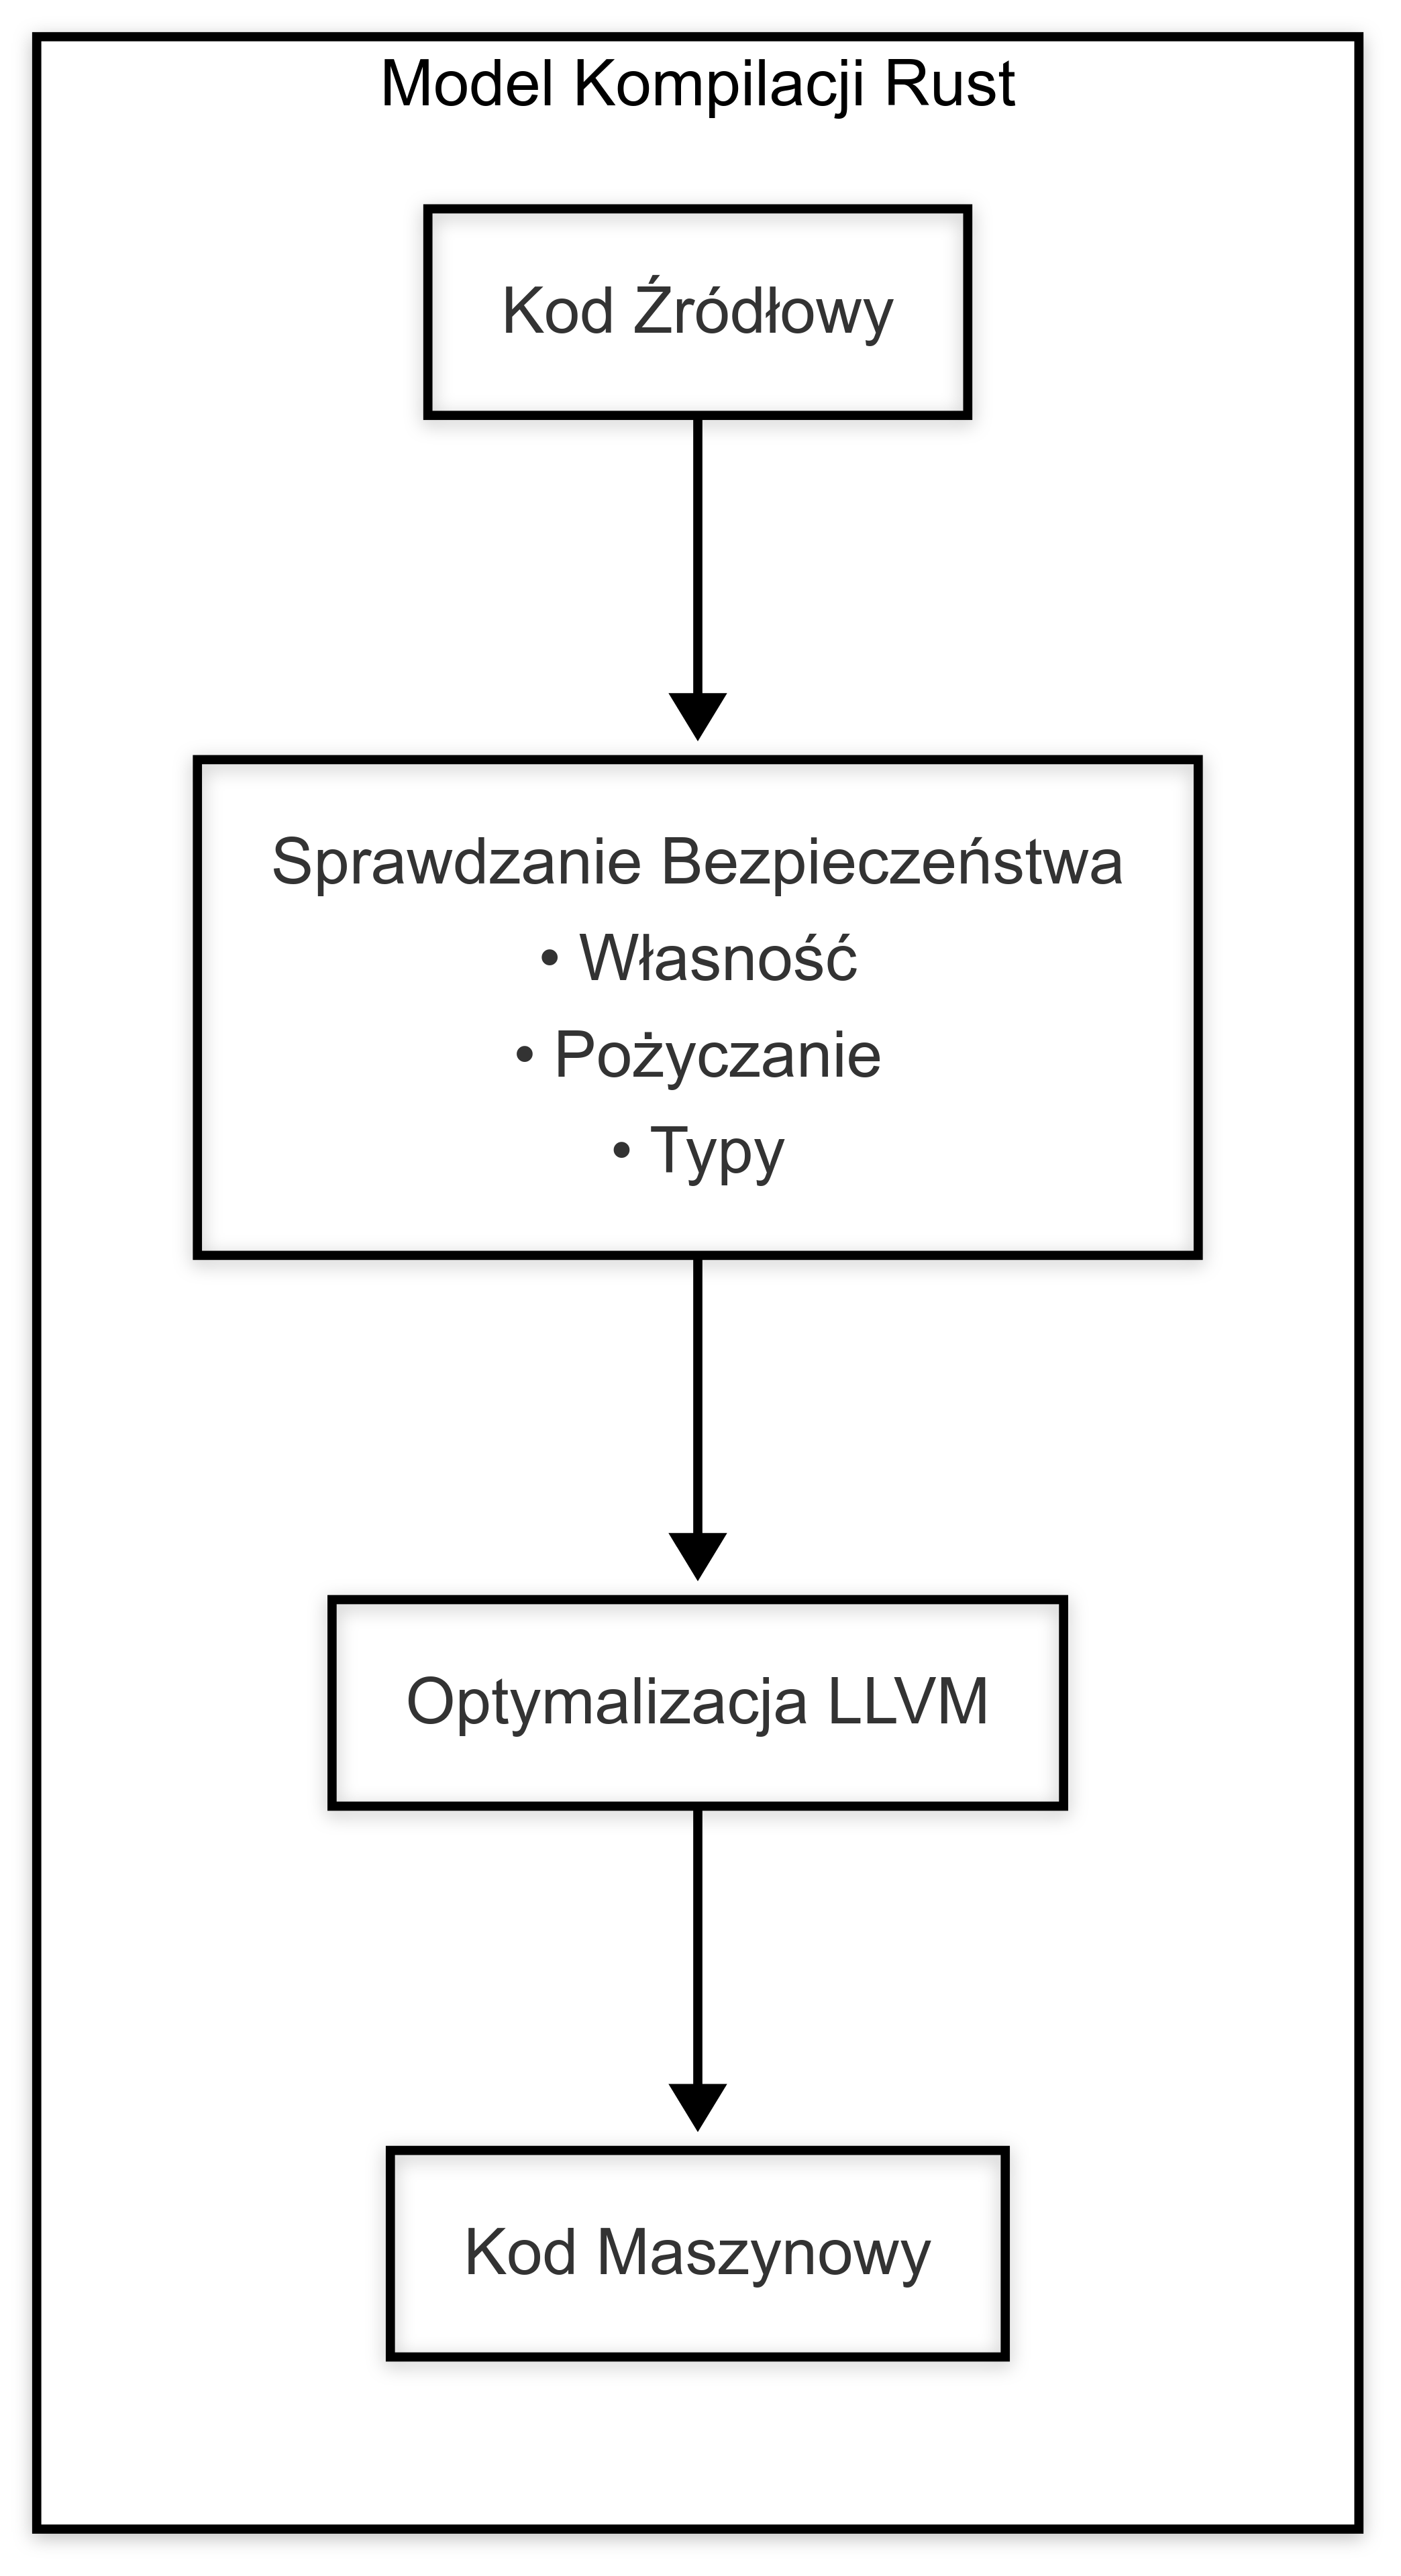
\includegraphics[height=12cm]{images/RustBuildsSteps.png}
        \caption{Kroki kompilacji w języku Rust}
        \label{fig:rust_build_steps}
    \end{minipage}%
    \begin{minipage}{.5\textwidth}
        \centering
        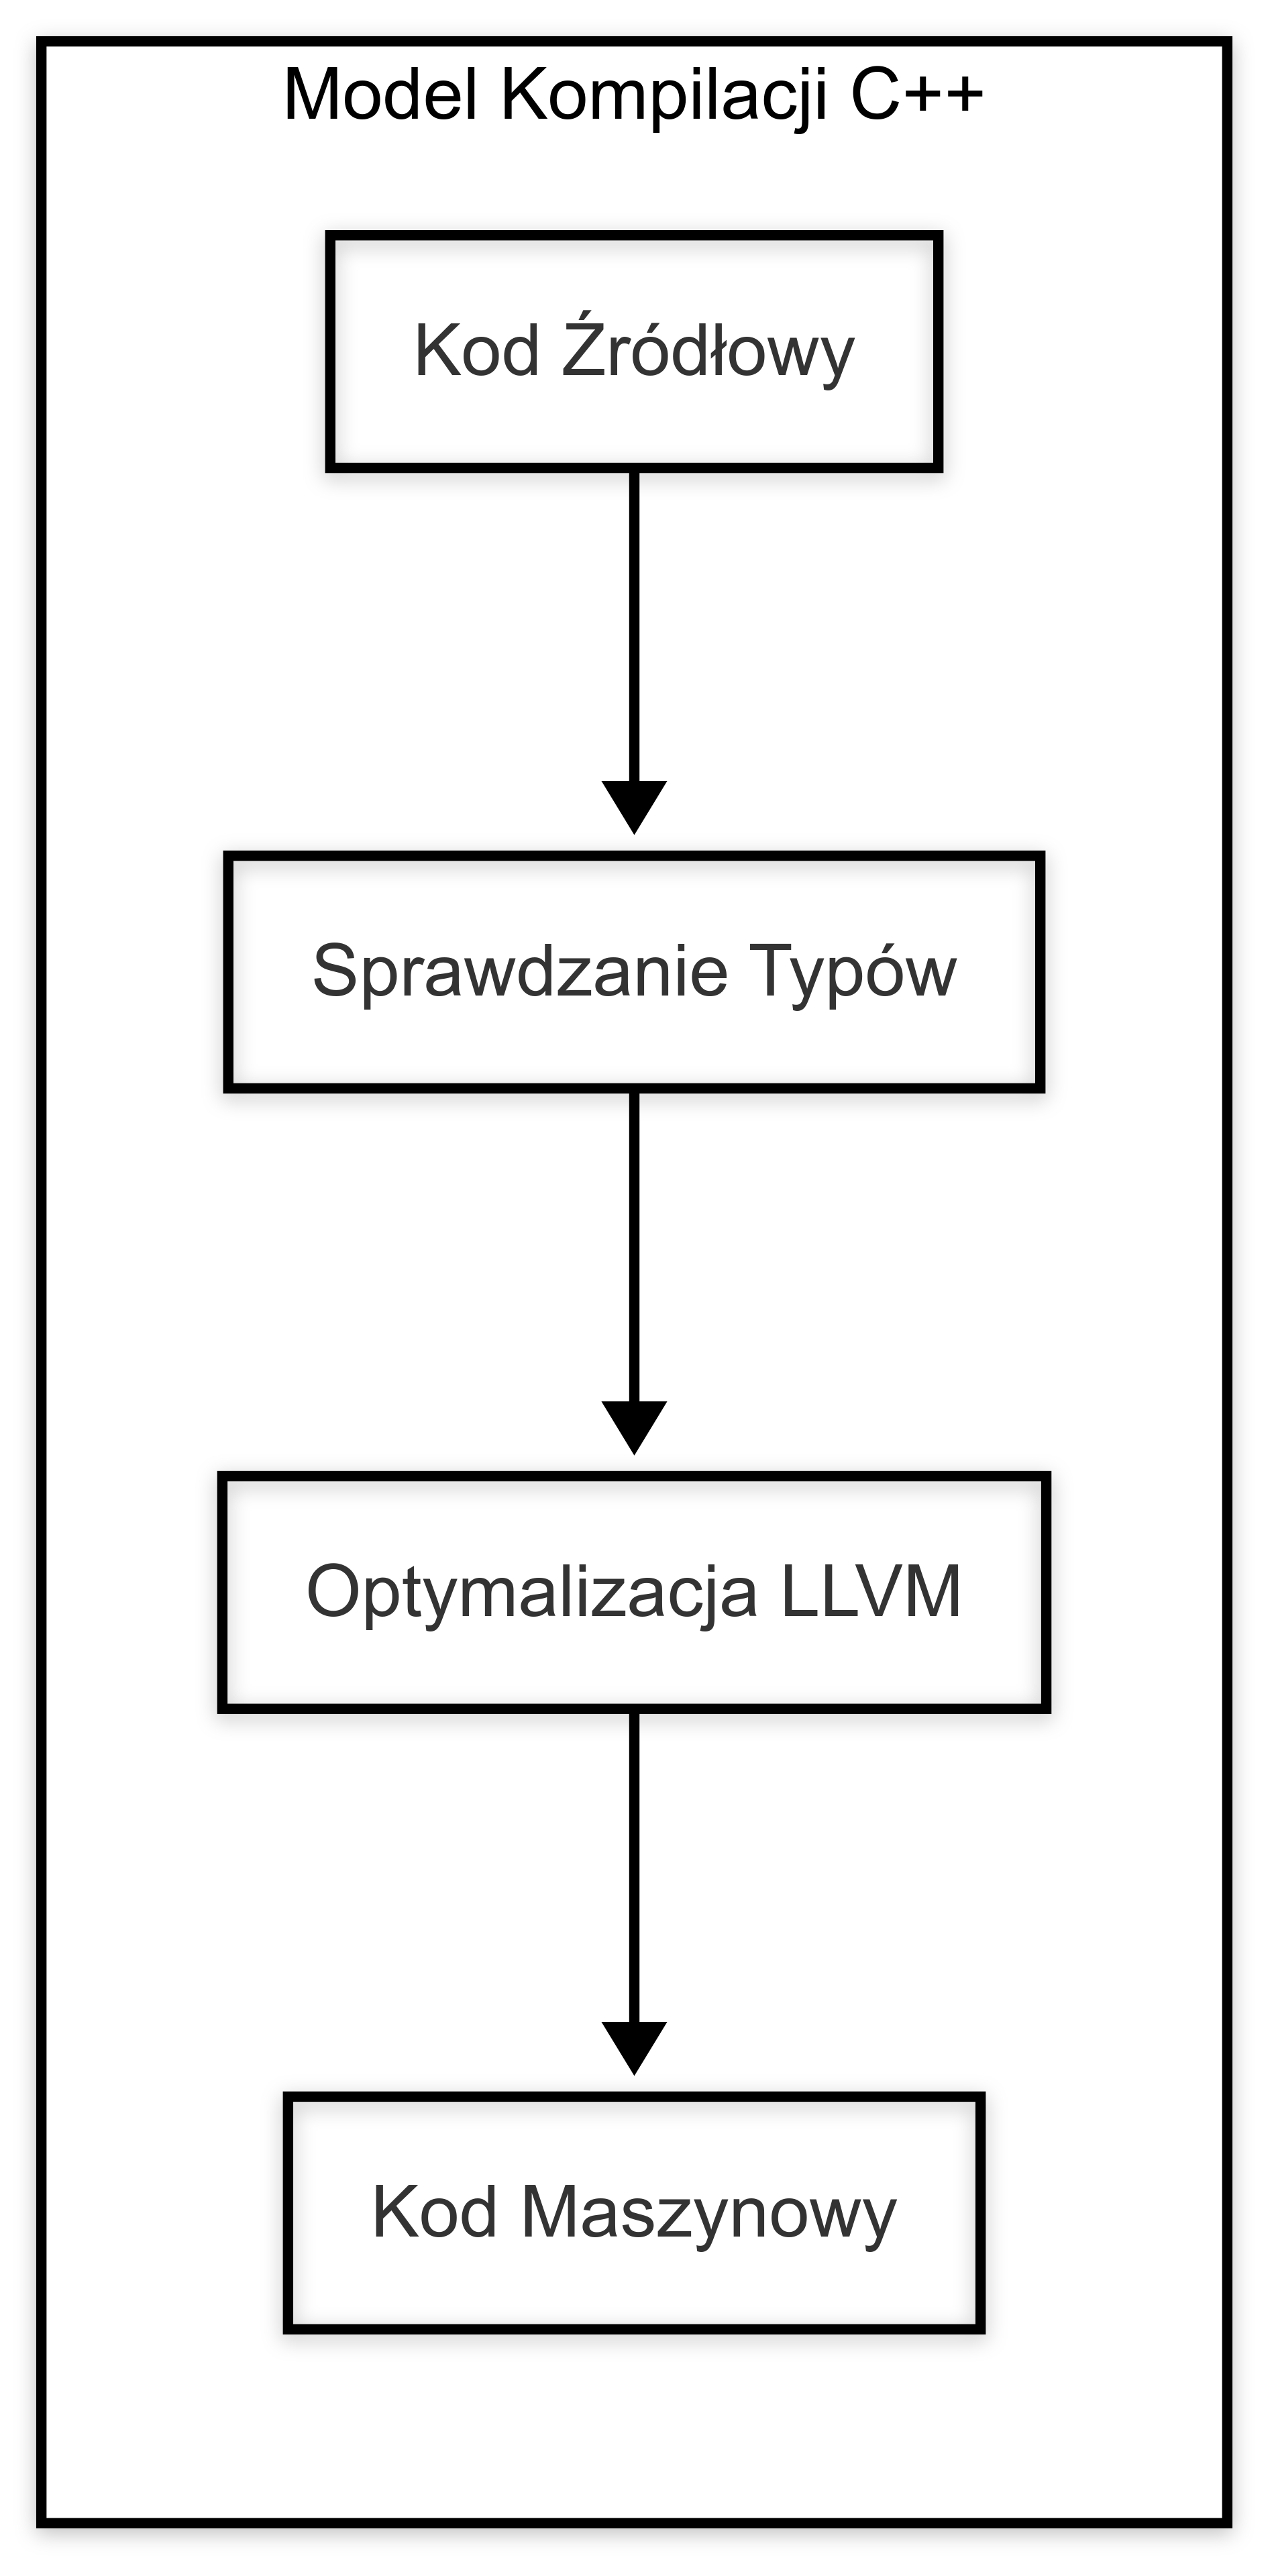
\includegraphics[height=12cm]{images/CppBuildsSteps.png}
        \caption{Kroki kompilacji w języku C++}
        \label{fig:cpp_build_steps}
    \end{minipage}
\end{figure}

Informacje o procesie kompilacji pochodzą z \cite{Lesiński, rustPolishNames, TheRustProgrammingLanguage}, które opisują integrację z LLVM i różnice w sprawdzaniu bezpieczeństwa.
Na rysunku \ref{fig:rust_build_steps} drugi blok reprezentuje dodatkowe etapy sprawdzania bezpieczeństwa w Rust, które nie występują w C++. Z kolei na rysunku \ref{fig:cpp_build_steps} drugi blok pokazuje podstawowe sprawdzanie typów w C++, które jest mniej rygorystyczne niż system Rust. Ze względu na różnicę w procesie kompulacji kodu powstają główne różnice w~bezpieczeństwie i wydajności obu języków.

C++ nadal pozostaje językiem preferowanym w projektach o krytycznym znaczeniu wydajnościowym, takich jak gry komputerowe, symulacje fizyczne czy systemy wbudowane, choć Rust zaczyna zdobywać popularność w tych obszarach ze względu na większe bezpieczeństwo przy porównywalnej wydajności. 

\subsection{Programowanie współbieżne oraz równoległe}
\label{Współbieżność}
Współbieżność i równoległość to kluczowe elementy programowania w  językach Rust i C++. Oba języki oferują zaawansowane narzędzia i biblioteki do zarządzania wielowątkowością.

Rust wyróżnia się systemem własności \eng{ownership} i wbudowanym mechanizmem wykrywania błędów współbieżności, co eliminuje wyścigi danych w czasie kompilacji. Narzędzia takie jak Tokio i Rayon pozwalają na łatwe tworzenie i zarządzanie zadaniami asynchronicznymi i równoległymi \cite{HandsOnConcurrencywithRust, RapidInnovationMasteringRust}.
C++ z kolei oferuje wsparcie dla wielowątkowości poprzez standardową bibliotekę (std::thread) oraz zaawansowane szkielety aplikacyjne (frameworks), takie jak OpenMP czy TBB (Threading Building Blocks). Chociaż te narzędzia są niezwykle potężne, nie zapewniają automatycznej ochrony przed błędami współbieżności, co wymaga większej ostrożności ze strony programistów.

Strona \cite{parallelrustcppIntroductionComparing} szczegółowo analizuje różnice w podejściu do współbieżności w obu językach, podkreślając, że Rust dzięki swojemu modelowi zarządzania pamięcią oferuje większe bezpieczeństwo, podczas gdy C++ pozostaje bardziej elastyczny, co może być korzystne w bardziej specyficznych scenariuszach. Jednak jak sam autor \cite{parallelrustcppIntroductionComparing} wskazuje, należy zwrócić uwagę, że większość sztuczek optymalizacyjnych pokazanych w tym porównaniu to jedynie adaptacje oryginalnych rozwiązań C++ w języku Rust. Koncentruje się ona na praktycznym porównaniu języków Rust i C++ pod względem równoległego przetwarzania, szczególnie na poziomie niskopoziomowych operacji i synchronizacji wątków. Znajdują się tam benchmarki pokazujące różnice w czasie wykonywania programów, narzędzia diagnostyczne oraz zestawienie wydajności w kontekście SIMD, wątków, oraz komunikacji międzypamięciowej.

W pracy akademickiej Brandefelta i Heymana \cite{heyman2020comparison} dokonano porównania wydajności oraz złożoności implementacyjnej aplikacji wielowątkowej napisanej w trzech językach: Rust, C++ oraz Java. Badanie to wykazało, że Rust oferuje zbliżoną wydajność do C++, przy jednoczesnym znacznym uproszczeniu kodu (mniejsza liczba linii kodu), co przekłada się na łatwiejsze utrzymanie i potencjalnie mniejszą podatność na błędy. Autorzy wskazują, że Rust, dzięki swojemu systemowi własności \eng{ownership}, eliminuje całe klasy błędów związanych z zarządzaniem pamięcią, bez konieczności stosowania odśmiecania.

Kolejne istotne opracowanie przedstawiono w publikacji Martinsa et al. \cite{martins2025npbrustnasparallelbenchmarks}, gdzie zaprezentowano implementację zestawu NAS (NASA Advanced Supercomputing) Parallel Benchmarks (NPB) \cite{nasaParallelBenchmarks} w języku Rust. Zestaw NPB stanowi uznany w środowisku naukowym standard do oceny wydajności systemów równoległych. W badaniach wykazano, że Rust osiąga porównywalną, a miejscami wyższą wydajność względem C++ i Fortranu (w wersjach OpenMP i~sekwencyjnych), co wskazuje na jego rosnący potencjał w dziedzinie wysokowydajnych obliczeń (HPC - High-Performance Computing). Jednocześnie zwrócono uwagę na trudności implementacyjne, związane z restrykcyjnym modelem bezpieczeństwa języka Rust, które jednak mogą być złagodzone poprzez zastosowanie odpowiednich bibliotek (np. Rayon).

Równolegle, w pracy Besozziego \cite{Besozzi} zaprezentowano bibliotekę Parallelo Parallel Library (PPL) - autorskie rozwiązanie do strukturalnego programowania równoległego w języku Rust. Biblioteka ta opiera się na wzorcach programowania równoległego takich jak szkielety \eng{skeletons} i wzorce projektowe, oferując wysokopoziomowe abstrakcje ułatwiające implementację złożonych aplikacji równoległych. Przeprowadzone testy wykazały, że PPL dorównuje lub przewyższa popularne biblioteki takie jak Rayon, jednocześnie zachowując zgodność z idiomami języka Rust i zasadą \textit{fearless concurrency}. Zastosowanie takich abstrakcji sprzyja zwiększeniu czytelności i poprawności kodu, co może mieć szczególne znaczenie w kontekście projektów systemowych.

Można również znaleźć pracę, która przedstawia wykorzystanie biblioteki odpowiedzialnej za współbieżność FastFlow przez oba języki Rust oraz C++ \cite{FastFlow}. Pokazuje ona, że język Rust jest dobrą alternatywą dla języka C++ w kontekście współbieżności.

% W odniesieniu do artykułów, czasopism oraz materiałów konferencyjnych opublikowanych w latach 2012 \footnotemark-2024, zidentyfikowanie prac, które jednoznacznie koncentrują się na problematyce pracy, jest wyzwaniem. Można natomiast znaleźć publikacje, które wykorzystują wspomniane języki (Rust oraz C++) i ich porównanie w kontekście złożonym do problemu pracy - chociażby wykorzystanie języka Rust w programowaniu układów wbudowanych \cite{ZamiennikWEmbedded}, jako zamiennik dla dotychczasowych języków z rodziny C.\\
% 
% \footnotetext{Rust został zaprezentowany w 2012 roku \cite{wikipediaRustprogramming}, a C++ w 1985 roku \cite{wikipediaWikipedia}.}


\section{Podsumowanie}
Na podstawie przeglądu literatury oraz zadanych pytań do przeglądu literatury można wskazać następujące odpowiedzi:
\subsubsection{PPL1: Jakie główne koncepcje/teorie dominują w literaturze dotyczącej porównania języków Rust oraz C++?}
W literaturze dominują badania porównawcze bezpieczeństwa, wydajności oraz zarządzania pamięcią w językach Rust i C++ - bardziej szczegółowo opisane w podrozdziałach \ref{Bezpieczeństwo} oraz \ref{CzasWykonania}. W kontekście współbieżności i równoległości można zauważyć znaczący wzrost prac w ubiegłych latach, co przedstawia przegląd opisany w podrozdziale \ref{Współbieżność}.

\subsubsection{PPL2: Jakie metody badawcze są najczęściej stosowane do analizy różnic pomiędzy językami ?}
W literaturze oraz w dotychczasowych analizach \cite{LanguageComparison_1,LanguageComparison_2,LanguageComparison_3,LanguageComparison_4} wskazano szereg kryteriów istotnych przy porównywaniu lub ocenie języków programowania ogólnego przeznaczenia. Do najważniejszych należą: 
    \begin{itemize}
        \item Prostota konstrukcji języka, mająca bezpośredni wpływ na łatwość programowania i zrozumiałość kodu.
        \item Czytelność kodu, związana z jego późniejszą konserwacją i rozwijaniem.
        \item Dostosowanie języka do konkretnego zastosowania, co wpływa na wydajność i efektywność programów.
        \item Szybkość kompilacji.
        \item Efektywność działania programu, zarówno pod względem szybkości, jak i zużycia zasobów systemowych.
        \item Dostępność i jakość bibliotek, frameworków oraz narzędzi wspierających rozwój oprogramowania.
        \item Wsparcie w procesie debugowania, profilowania i testowania kodu.
        \item Bezpieczeństwo języka, związane z eliminacją błędów w czasie kompilacji oraz wykrywaniem zagrożeń w trakcie działania programu.
        \item Długowieczność języka oraz narzędzi kompilacyjnych, co wpływa na stabilność i przewidywalność rozwoju oprogramowania.
        \item Przenośność między różnymi platformami i architekturami sprzętowymi.
    \end{itemize}
    Wszystkie te kryteria mają istotny wpływ na całkowity koszt i nakład pracy związany z tworzeniem oraz utrzymaniem oprogramowania, a także na jego jakość i przydatność w długim okresie użytkowania.

    Doświadczenie wskazuje również, że te same kryteria można stosować do oceny innych komponentów wspomagających proces tworzenia oprogramowania, takich jak biblioteki klas obiektowych czy projekty typów abstrakcyjnych. Wykorzystanie odpowiednich, zewnętrznych komponentów oraz dobrze zaprojektowanych rozwiązań przyczynia się do poprawy czytelności, utrzymywalności i ogólnej jakości kodu, jednocześnie przyspieszając proces jego tworzenia.

\subsubsection{PPL3: Jak wygląda porównanie dostępności i dojrzałości bibliotek do programowania współbieżnego i równoległego w obu językach?}
Porównując dostępność i dojrzałość bibliotek do programowania współbieżnego i równoległego w językach Rust i C++, zauważyć można istotne różnice wynikające zarówno z historii rozwoju tych języków, jak i ich podejścia do bezpieczeństwa, abstrakcji oraz zarządzania zasobami.

W przypadku języka C++, biblioteki takie jak OpenMP, Intel TBB czy pthreads cechują się dużą dojrzałością oraz szerokim zastosowaniem w przemyśle, zwłaszcza w kontekście obliczeń naukowych, symulacji fizycznych i systemów o wysokiej wydajności. Są one dobrze udokumentowane, posiadają wsparcie komercyjne (np. TBB) oraz charakteryzują się dużą kompatybilnością z istniejącą infrastrukturą sprzętową i programową. Niemniej jednak, wymagają od programisty głębokiej wiedzy w zakresie zarządzania pamięcią oraz synchronizacji, co przekłada się na wyższy próg wejścia i podatność na błędy (np. wyścigi danych czy zakleszczenia).

Z kolei Rust, jako język nowszy, oferuje bardziej nowoczesny zestaw narzędzi do programowania równoległego, w tym biblioteki takie jak Tokio, Rayon czy Crossbeam. Mimo mniejszej liczby lat rozwoju, biblioteki te szybko dojrzewają i zdobywają popularność dzięki silnym gwarancjom bezpieczeństwa pamięci na poziomie kompilatora oraz ergonomicznemu API. Rust promuje bezpieczne podejście do współbieżności poprzez system własności \eng{ownership} i brak domyślnego współdzielenia zasobów, co w praktyce eliminuje całą klasę błędów typowych dla C++. Dzięki temu biblioteki w Rust, choć mniej rozpowszechnione w starszych zastosowaniach, zyskują przewagę w projektach tworzonych od podstaw, zwłaszcza w środowiskach wymagających wysokiej niezawodności.

\subsubsection{PPL4: Czy istnieją systematyczne metodologie porównywania języków programowania w kontekście problemu pracy, które można zastosować do analizy Rust i C++?}

W literaturze przedmiotu można znaleźć prace proponujące sformalizowane, systematyczne metodologie służące do porównywania języków programowania w kontekście ich wsparcia dla współbieżności i równoległości. Jednakzę zdecydowana większość badań skupia się na aspektach wydajnościowych, bezpieczeństwa pamięci lub ekspresyjności języka, dodatkowo często przyjmują one podejścia ad hoc, oparte na wybranych przypadkach użycia, bez spójnych ram metodologicznych.

Niektóre opracowania, jak np. porównania publikowane w ramach blogów technicznych czy artykułów na platformach takich jak Medium, wykorzystują podejścia oparte na konteneryzacji programów testowych i~ich uruchamianiu na jednorodnej infrastrukturze. Przykładowo, w~metodzie \textit{Rainbow} \cite{rainbow} badana jest przepustowość obliczeń przy wykorzystaniu kontenerów i~zewnętrznego systemu, jak Redis, do monitorowania wyników. Choć takie podejścia są ciekawe, narażone są na zakłócenia wynikające z różnic w czasie inicjalizacji kontenerów, rozmiarze obrazu czy użyciu pamięci, co może zafałszowywać końcowe wyniki porównawcze.

Znacznie bardziej sformalizowanym podejściem jest wykorzystanie ustandaryzowanych pakietów benchmarkowych, takich jak NAS Parallel Benchmarks (NPB), które zostały opracowane przez NASA w celu obiektywnej oceny wydajności systemów wieloprocesorowych. Przykładem zastosowania tej metodologii jest praca „NPB-Rust” \cite{martins2025npbrustnasparallelbenchmarks}, w której autorzy przeprowadzili systematyczne porównanie implementacji benchmarków NAS w języku Rust (z użyciem biblioteki Rayon) oraz C++ (z użyciem OpenMP). Ocenie poddano nie tylko wydajność obliczeniową, ale również skalowalność, zużycie pamięci oraz nakład implementacyjny, mierząc m.in. liczbę linii kodu i szacowany koszt harmonogramowania według modelu COCOMO - \eng{Constructive Cost Model} - to model szacowania kosztów związanych z rozwojem oprogramowania.

Takie podejścia, oparte na zweryfikowanych zestawach testowych, umożliwiają bardziej wiarygodne i powtarzalne porównania pomiędzy językami programowania w kontekście współbieżności i równoległości. W związku z tym, zastosowanie frameworków benchmarkowych takich jak NPB powinno być traktowane jako wzorzec dla przyszłych badań w tej dziedzinie.

\subsubsection{PPL5: Jakie aspekty programowania współbieżnego i równoległego w Rust i C++ nie zostały dostatecznie zbadane w literaturze?}
Dotychczasowe badania naukowe dotyczące programowania współbieżnego w językach Rust i C++ koncentrowały się przede wszystkim na ogólnych aspektach, takich jak bezpieczeństwo pamięci, kontrola dostępu do danych, ergonomia kodu oraz wydajność kompilacji i wykonania. W szczególności analizowano podejście języków do eliminacji błędów wykonawczych (np. data races), mechanizmy typizacji oraz zarządzanie zasobami systemowymi. Przykładem mogą być prace \cite{heyman2020comparison}, które zestawiają Rust i C++ w kontekście praktycznych implementacji aplikacji wielowątkowych, czy badania \cite{martins2025npbrustnasparallelbenchmarks}, porównujące implementacje benchmarków równoległych.

Niemniej jednak, najnowsze publikacje wskazują na wypełnienie wielu wcześniej istniejących luk, zwłaszcza w zakresie porównania konkretnych konstrukcji językowych \linebreak (np. \mbox{async/await} kanały, skeletons) oraz empirycznej weryfikacji wydajności bibliotek wspierających równoległość (np. PPL, Rayon, OpenMP).

Pomimo to, w literaturze wciąż można zidentyfikować kilka istotnych obszarów badawczych, które pozostają niewystarczająco zbadane:
\begin{itemize}
    \item \textbf{Wpływ architektury sprzętowej na zachowanie systemów współbieżnych:}\\
    Większość dotychczasowych badań prowadzono na klasycznych architekturach x86\_64. Brakuje natomiast analiz zachowania aplikacji wielowątkowych w Rust i C++ na alternatywnych platformach, takich jak ARM, RISC-V czy systemy heterogeniczne (np. SoC zawierające zarówno CPU, jak i akceleratory). Tego typu analizy są szczególnie istotne w kontekście rozwoju systemów wbudowanych oraz IoT, gdzie Rust zyskuje coraz większą popularność.
    \item \textbf{Koszt abstrakcji oraz narzut związany z modelem bezpieczeństwa Rust:}\\
    Choć bezpieczeństwo współbieżności w Rust jest jego kluczowym atutem, literatura rzadko podejmuje próbę precyzyjnego oszacowania narzutu wydajnościowego wynikającego z jego rygorystycznego modelu własności i sprawdzania pożyczeń. Istnieje potrzeba eksperymentalnych badań porównawczych, które wykazałyby, w jakim stopniu koszt ten wpływa na skalowalność aplikacji w środowiskach o dużym współczynniku równoległości.
    \item \textbf{Porównanie ergonomii rozwiązań współbieżnych na poziomie idiomatycznym i bibliotekowym:}\\
    Chociaż wiele prac omawia techniczne możliwości języków (np. \texttt{std::thread}, Tokio, OpenMP, \texttt{std::thread} w C++), nadal brakuje badań jakościowych dotyczących ergonomii kodu, łatwości diagnostyki błędów oraz odporności na błędy logiczne podczas implementacji systemów wielowątkowych. Takie analizy mogłyby obejmować porównania idiomatycznych podejść (np. actor model, CSP, fork-join), oferowanych przez biblioteki Rust i C++.
    \item \textbf{Zachowanie systemów współbieżnych w warunkach zmiennego obciążenia i konkurencyjnego dostępu:}\\
    Istnieje luka w badaniach dotyczących stabilności i odporności aplikacji na skoki obciążenia lub dynamiczną alokację wątków. Potrzebne są badania stresowe i profilowanie systemów w~warunkach rzeczywistej konkurencji (np. serwery HTTP, silniki obliczeniowe), co pozwoliłoby ocenić adaptacyjność strategii planowania i zarządzania wątkami w Rust i C++.
    \item \textbf{Weryfikacja formalna i modelowanie błędów współbieżności:}\\
    Pomimo iż język Rust oferuje silne gwarancje bezpieczeństwa na etapie kompilacji - statyczna gwarancja bezpieczeństwa, zagadnienia związane z formalną weryfikacją własności współbieżnych, takich jak żywotność \eng{liveness}, brak zagłodzenia \eng{starvation-freedom} czy deterministyczność wykonania, pozostają w literaturze stosunkowo słabo zbadane. Potencjalnie wartościowym kierunkiem dalszych analiz byłoby porównanie dostępnych narzędzi formalnych, takich jak weryfikatory modeli, w kontekście języka Rust oraz innych języków programowania współbieżnego. Tego rodzaju zestawienie mogłoby przyczynić się do lepszego zrozumienia możliwości i ograniczeń istniejących podejść do formalnej weryfikacji w~środowiskach wielowątkowych.
\end{itemize}


\subsubsection{PPL6: Jaki jest stan wiedzy na temat wykorzystania programowania współbieżnego w ramach GPU w językach Rust i C++?}
W literaturze przedmiotowej oraz w praktyce programistycznej, zagadnienie wykorzystania programowania współbieżnego na GPU ewoluuje w różnym tempie w zależności od języka programowania. W przypadku języka Rust obserwujemy dynamiczny rozwój narzędzi, które umożliwiają wykorzystanie mocy obliczeniowej kart graficznych przy jednoczesnym zachowaniu wysokich gwarancji bezpieczeństwa pamięci i wątków.

Projekty takie jak rust-gpu \cite{rustgpuRust} dążą do umożliwienia pisania programów cieniujących w języku Rust, oferując podejście, które integruje możliwości GPU z bezpiecznymi konstrukcjami języka. Dokumentacja dostępna na stronie github \cite{rustgpuRust} wskazuje na intensywne prace nad przeniesieniem wielu korzyści wynikających z systemu własności i typizacji Rust na środowisko GPU, co może przyczynić się do zmniejszenia ryzyka błędów współbieżności, które są szczególnie krytyczne w obliczeniach równoległych.

Równolegle, biblioteka Vulkano (dostępna m.in. poprzez dokumentację \cite{docsVulkanoRust}) stanowi wysokopoziomowy, bezpieczny interfejs do API Vulkan, które jest standardem w programowaniu GPU. Vulkano umożliwia abstrakcję złożoności niskopoziomowych interfejsów, jednocześnie oferując możliwość pełnego wykorzystania równoległości GPU. W podobnym nurcie znajduje się projekt wgpu, który implementuje standard WebGPU, umożliwiając przenośne aplikacje graficzne i obliczeniowe, a jednocześnie integrując współczesne podejścia do zarządzania zasobami i synchronizacji.

W przeciwieństwie do podejścia Rust, w środowisku C++ dominującym rozwiązaniem jest platforma CUDA, rozwijana i wspierana przez firmę NVIDIA \cite{nvidiaCUDAToolkit}. CUDA oferuje bardzo dojrzały, zoptymalizowany i szeroko stosowany framework, który pozwala na bezpośrednią implementację algorytmów równoległych na GPU. W odróżnieniu od narzędzi rozwijanych dla Rust, CUDA posiada ugruntowaną pozycję w środowisku przemysłowym, co przekłada się na bogatą dokumentację, szerokie wsparcie techniczne oraz liczne biblioteki wspomagające rozwój aplikacji wykorzystujących GPU.

Podsumowując, stan wiedzy dotyczący programowania współbieżnego na GPU w języku Rust znajduje się na etapie intensywnego rozwoju i eksperymentacji, gdzie projekty takie jak rust-gpu, Vulkano oraz wgpu \cite{wgpuWgpuPortable} pokazują potencjał tego podejścia, zwłaszcza w kontekście bezpieczeństwa i nowoczesnych abstrakcji. Z kolei w C++ platforma CUDA, dzięki swojej dojrzałości oraz szerokiemu wsparciu ze strony przemysłu, pozostaje głównym narzędziem wykorzystywanym do implementacji wysokowydajnych obliczeń równoległych na GPU.

\subsection{Kierunki dalszych badań}
Na podstawie przeglądu literatury oraz odpowiedzi na pytania do przeglądu literatury można wskazać na kilka kierunków dalszych badań w dziedzinie programowania współbieżnego i równoległego w językach Rust i C++:
\begin{itemize}
    \item \textbf{Rozszerzone porównania systematyczne mechanizmów współbieżnych i równoległych} — z uwzględnieniem nie tylko wydajności, ale także ergonomii, bezpieczeństwa pamięci, ekspresyjności kodu oraz kosztu implementacyjnego.
    \item \textbf{Analiza porównawcza konkretnych mechanizmów i bibliotek} — takich jak \texttt{std::thread} w C++ i Rust, \texttt{OpenMP} a \texttt{Rayon}, czy też mechanizmy asynchroniczne (\texttt{async/await} w Rust a \texttt{futures}, \texttt{std::coroutine} w C++20 i nowszych).
    \item \textbf{Analiza wpływu zastosowania unsafe code w Rust} — w kontekście uzyskiwanej wydajności i kompromisów względem bezpieczeństwa pamięci oraz czytelności kodu.
    \item \textbf{Zastosowania programowania równoległego na GPU} — porównanie możliwości Rust (np. poprzez biblioteki takie jak \texttt{rust-gpu} czy \texttt{wgpu}) z rozwiązaniami dostępnymi w ekosystemie C++ (np. CUDA, SYCL, OpenCL).
    \item \textbf{Badanie wpływu konstrukcji językowych na podatność na błędy współbieżności} — \mbox{np. warunki} wyścigu, zakleszczenia, użycie nieprawidłowych referencji lub wskaźników, z~uwzględnieniem poziomu ochrony oferowanego przez kompilator.
\end{itemize}

\chapter{Przegląd literatury}
Celem niniejszego rozdziału jest przedstawienie dotychczasowych badań i publikacji dotyczących mechanizmów programowania współbieżnego i równoległego w językach Rust i C++. Analiza literatury umożliwi zrozumienie aktualnego stanu wiedzy w tej dziedzinie, a także wskazanie na występujące luki badawcze, które niniejsza praca postara się wypełnić.
Na samym wstępie zostały postawione następujące pytania do przeglądu literatury, które pomogą zrozumieć oraz sprawdzić aktualny stan wiedzy jeżeli chodzi o porównanie języków Rust oraz C++:

\begin{quote}
    \item \textbf{PPL1:} \emph{Jakie główne koncepcje/teorie dominują w literaturze dotyczącej porównania języków Rust oraz C++?}
    \item \textbf{PPL2:} \emph{Jakie metody badawcze są najczęściej stosowane do analizy różnic pomiędzy językami ?}
    \item \textbf{PPL3:} \emph{Jak wygląda porównanie dostępności i dojrzałości bibliotek do programowania współbieżnego i równoległego w obu językach?}
    \item \textbf{PPL4:} \emph{Czy istnieją systematyczne metodologie porównywania języków programowania w kontekście współbieżności, które można zastosować do analizy Rust i C++?}
    \item \textbf{PPL5:} \emph{Jakie aspekty programowania współbieżnego i równoległego w Rust i C++ nie zostały dostatecznie zbadane w literaturze?}
    \item \textbf{PPL6:} \emph{Jaki jest stan wiedzy na temat wykorzystania programowania współbieżnego w ramach GPU w językach Rust i C++?}
\end{quote}

Odpowiedzi na powyższe pytania pozwolą na zidentyfikowanie kluczowych obszarów, które wymagają dalszych badań oraz na wskazanie na potencjalne kierunki rozwoju w dziedzinie programowania współbieżnego i równoległego w językach Rust i C++.\\
Przegląd literatury odbywał się z wykorzystaniem narzędzi baz danych oferujących wyszukiwanie, filtrowanie oraz przegląd prac: Scopus, Google Scholar.\\
W ramach bazy scopus wykorzystano następujące kwerendy do wyszukiwania - tabela \ref{table:literatureReviewQueries}

\begin{table}[H]
    \caption{Kwerendy użyte w bazie Scopus \protect \footnotemark}
    \label{table:literatureReviewQueries}
    \begin{tabular}{|c|p{11cm}|c|}
    \hline
    Lp. & Kwerenda & Liczba wyników \\ \hline
    1 & ALL ("concurrent programming"\ OR "parallel programming") AND (ALL ("Rust") AND ALL ("C++")) & 444 \\ \hline

    2 & ALL ("concurrent programming"\ OR "parallel programming") AND (ALL ("Rust") AND ALL ("C++") ) AND ( ALL ("compare")) & 28 \\ \hline

    3 & (TITLE-ABS-KEY(("concurrent programming"\ OR "parallel programming") AND ("Rust"\ AND "C++"))) AND (TITLE-ABS-KEY("comparison"\ OR "evaluation"\ OR "benchmark")) & 6 \\ \hline

    4 & (TITLE-ABS-KEY(("thread"\ OR "async"\ OR "future"\ OR "actor model"\ OR "message passing"\ OR "shared memory") AND ("Rust"\ AND "C++"))) AND (TITLE-ABS-KEY("comparison"\ OR "performance"\ OR "evaluation")) & 50 \\ \hline

    5 & (TITLE-ABS-KEY(("Rust"\ AND "C++") AND ("concurrency model"\ OR "parallel constructs"\ OR "multithreading"))) AND (TITLE-ABS-KEY("comparison"\ OR "study")) & 2 \\ \hline

    \end{tabular}
\end{table}
\footnotetext{Ilość wyników dla poszczególnych zapytań może się różnić w zależności od daty (wyszukiwanie przeprowadzono w okresie listopad-luty 2024/25).}

W celu identyfikacji literatury związanej z porównaniem wybranych mechanizmów programowania współbieżnego i równoległego w językach Rust i C++, opracowano pięć zapytań w bazie Scopus, z których każde miało określony cel badawczy. Pierwsze zapytanie miało na celu uzyskanie ogólnego przeglądu literatury, wyszukując wszystkie dokumenty, w których występują jednocześnie zagadnienia programowania współbieżnego lub równoległego oraz języki Rust i C++, niezależnie od kontekstu. Pozwoliło to oszacować ogólną skalę badań łączących te zagadnienia. Drugie zapytanie zawężało zakres wyszukiwania poprzez dodanie słowa kluczowego „compare”, co umożliwiło wyodrębnienie publikacji, w których dokonano bezpośredniego porównania języków Rust i C++ w kontekście współbieżności lub równoległości. Dzięki temu uzyskano bardziej ukierunkowany zbiór literatury odnoszącej się do analizy porównawczej. Trzecie zapytanie charakteryzowało się większą precyzją, ograniczając wyniki do tytułów, streszczeń oraz słów kluczowych, i uwzględniało wyłącznie publikacje zawierające odniesienia do ewaluacji, porównań bądź benchmarków języków Rust i C++. Takie podejście pozwoliło wyselekcjonować najbardziej tematycznie powiązane prace. Czwarte zapytanie miało charakter bardziej techniczny, koncentrując się na konkretnych mechanizmach współbieżności, takich jak wątki, asynchroniczność, obiekty typu futury, model aktorów, przesyłanie komunikatów czy pamięć współdzielona, w połączeniu z terminami dotyczącymi wydajności i oceny. Umożliwiło to dotarcie do badań analizujących niskopoziomowe aspekty działania tych mechanizmów w obu językach. Piąte zapytanie skupiało się na poziomie koncepcyjnym, wyszukując publikacje zawierające takie terminy jak model współbieżności, konstrukty równoległe czy wielowątkowość, wraz z frazami dotyczącymi porównań lub analiz. Celem było zidentyfikowanie prac badających różnice w podejściu do współbieżności na poziomie architektury języka i jego konstrukcji wewnętrznych.

Autor zdecydował się również użyć nowego, wbudowane narzędzia w systemie Scopus - Scopus AI. Narzędzie to oparte na sztucznej inteligencji, wspomaga eksplorację akademicką w oparciu o dane z platformy Scopus. Dzięki integracji z narzędziem Copilot optymalizuje wyszukiwania, łącząc metody semantyczne i dopasowanie słów kluczowych. Choć Scopus AI ułatwia badania, jego wyniki warto weryfikować, ponieważ mogą zawierać nieścisłości lub stronniczość. \\
Po wprowadzeniu tytułu pracy w języku angielskim jako kwerendę, Scopus AI zwrócił 9 wyników, biorąc pod uwagę kwerendę stworzoną na podstawie tytyułu pracy, zamieszczoną w listingu \ref{AIQuery}. Zwrócone prace pokrywają się z przeglądem umieszczonym w tabeli \ref{table:literatureReviewQueries} 

\lstset{breaklines=true}
\begin{lstlisting}[caption=Kwerenda wygenerowana przez AI, label=AIQuery]
("concurrent programming" OR "parallel programming" OR "multithreading" OR "asynchronous")
AND ("Rust" OR "C++" OR "programming languages" OR "software development")
AND ("performance" OR "efficiency" OR "scalability" OR "resource management")
AND ("synchronization" OR "thread safety" OR "deadlock" OR "race condition")
AND ("libraries" OR "frameworks" OR "tools" OR "APIs")
\end{lstlisting}


\section{Porównanie Rust oraz C++}
Porównanie języków programowania Rust i C++ jest przedmiotem licznych publikacji, które analizują ich różnorodne aspekty, takie jak struktura kodu, sposób kompilacji, bezpieczeństwo, wydajność oraz obsługa współbieżności i równoległości. Niestety wśród prac naukowych zidentyfikowanych w bazach danych Scopus oraz Google Scholar, nie znaleziono prac, które jednoznacznie porównywałyby oba języki w kontekście programowania współbieżnego i równoległego.\\
W literaturze można znaleźć prace, które analizują różnice między Rustem a C++ w kontekście bezpieczeństwa, wydajności, zarządzania pamięcią oraz obsługi błędów.

\subsection{Bezpieczeństwo}
\label{Bezpieczeństwo}
Bezpieczeństwo języków Rust i C++ jest jednym z najczęściej analizowanych tematów w literaturze. W przypadku Rusta duży nacisk kładziony jest na eliminację całych klas błędów, takich jak null pointer dereferencing, data races oraz wycieki pamięci. Mechanizmy takie jak ownership, borrow checker oraz obowiązkowa mutowalność zmiennych (explicit mutability) są wymieniane jako kluczowe elementy zapewniające bezpieczeństwo oraz minimalizując ryzyko wycieków pamięci \cite{MigratingCtoRustforMemorySafety}. 

Z drugiej strony, C++ umożliwia większą kontrolę nad pamięcią, co może być zaletą w systemach wymagających maksymalnej wydajności, ale jednocześnie wiąże się z koniecznością samodzielnego zarządzania zasobami przez programistów. W literaturze \cite{RustDifferences, RustDifferences1} często podkreśla się, że to właśnie większa złożoność i ryzyko błędów w kodzie C++ skłoniły społeczność do stworzenia języków takich jak Rust.

Przykładowo, badania \cite{RustSafety1, RustSafety2, RustSafety3} wskazują, że aplikacje napisane w Rusta są mniej podatne na błędy związane z wyścigami danych \eng{data races}, co ma szczególne znaczenie w środowiskach wielowątkowych. Z kolei w C++ stosowanie bibliotek takich jak std::thread czy frameworków typu OpenMP pozwala na osiągnięcie podobnych celów, choć wymaga od programistów większej uwagi w zakresie synchronizacji. Dodatkowo są również prace \cite{PPL1_1,PPL1_2}, które przedstawiają próby implementacji mechanizmów wbudowanych w język Rust (prawo własności, pożyczka) do języka C.
\subsection{Czas wykonania}
\label{CzasWykonania}
Porównania czasów wykonania programów napisanych w Rust i C++ są częstym tematem analiz \cite{RustPerformance1, RustPerformance2, RustPerformance3, RustPerformance4}. W badaniach tych zostało wykazane, że pod względem wydajności Rust jest konkurencyjny wobec C++, co wynika z mechanizmów kompilacji i optymalizacji kodu.

Jednak kluczową różnicą jest to, że Rust wprowadza pewne narzuty związane z kontrolą bezpieczeństwa w czasie kompilacji, które mogą wydłużyć czas budowania programu, ale nie wpływają znacząco na czas wykonania.\\
Rust i C++ są językami kompilowanymi, co oznacza, że dedykowany kompilator tłumaczy kod źródłowy na kod maszynowy przed jego wykonaniem. Dzięki temu możliwe jest uzyskanie wysokiej wydajności programów. W literaturze \cite{Lesiński} często podkreśla się, że Rust, w odróżnieniu od C++, kładzie większy nacisk na bezpieczeństwo pamięci oraz typów w czasie kompilacji, co ma kluczowe znaczenie w nowoczesnym oprogramowaniu. W kontekście C++ wskazuje się na jego większą elastyczność oraz bogaty ekosystem, który pozwala na szeroką gamę zastosowań, ale jednocześnie wymaga większej uwagi programistów w zakresie zarządzania pamięcią i synchronizacji wątków.
% two images next to each other
\begin{figure}[H]
    \centering
    \begin{minipage}{.5\textwidth}
        \centering
        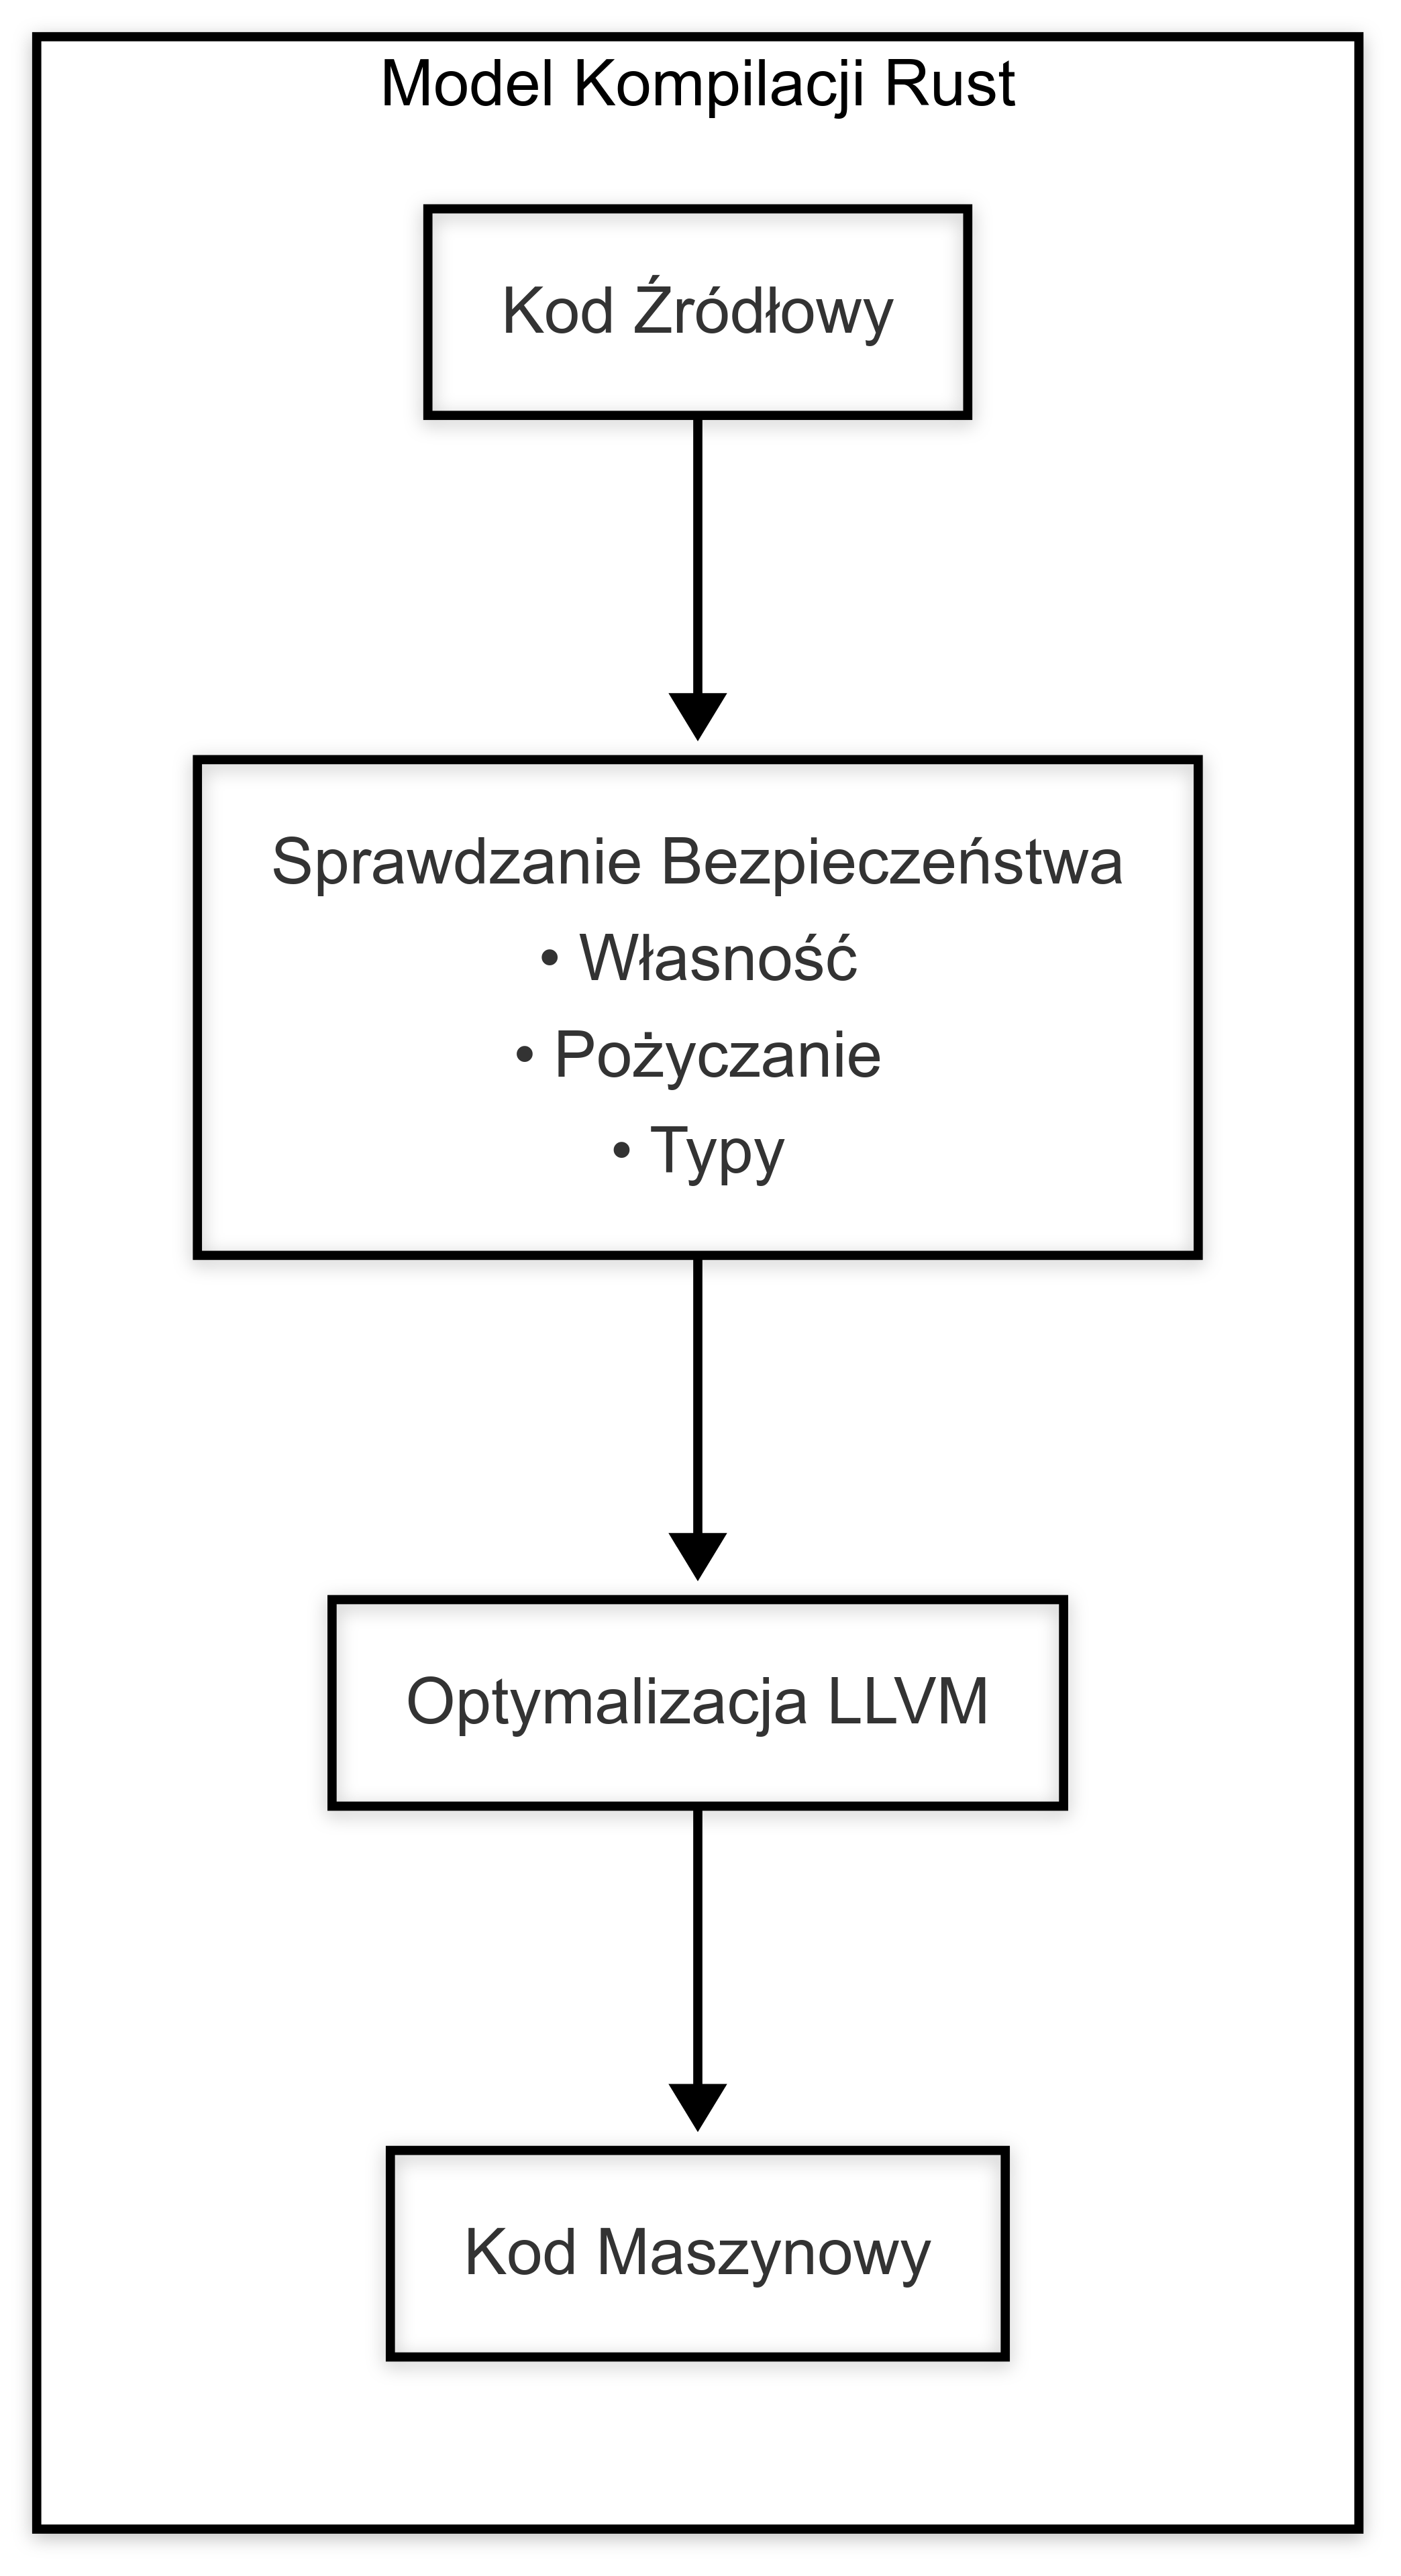
\includegraphics[height=12cm]{images/RustBuildsSteps.png}
        \caption{Kroki kompilacji w języku Rust}
        \label{fig:rust_build_steps}
    \end{minipage}%
    \begin{minipage}{.5\textwidth}
        \centering
        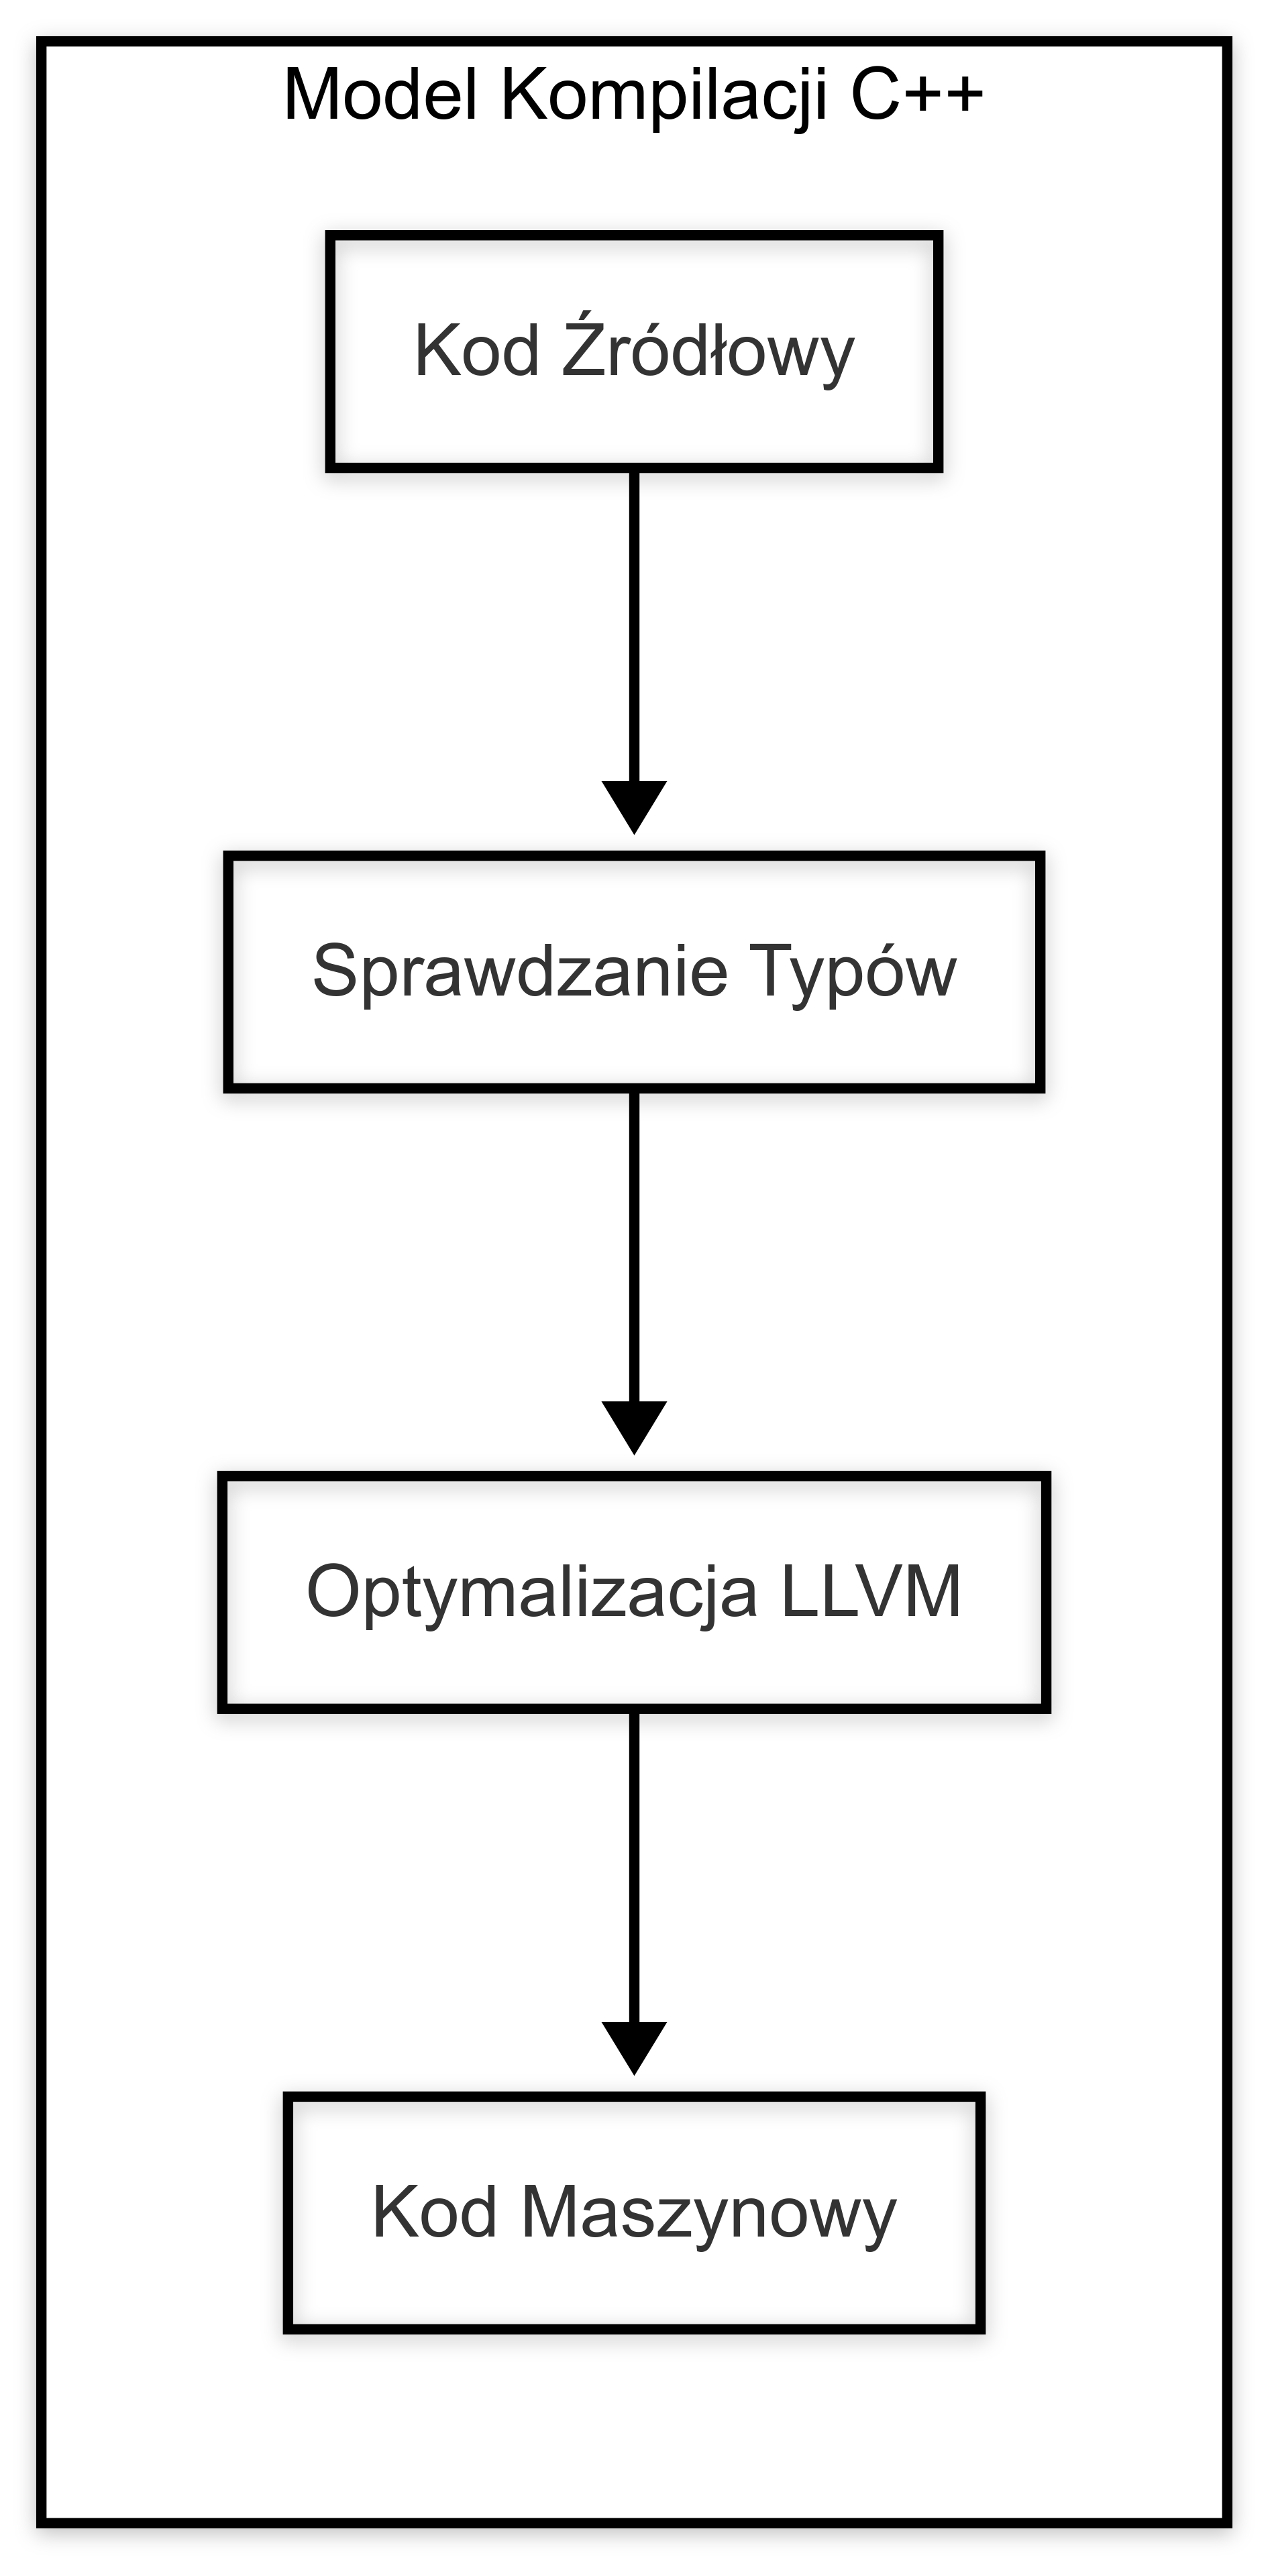
\includegraphics[height=12cm]{images/CppBuildsSteps.png}
        \caption{Kroki kompilacji w języku C++}
        \label{fig:cpp_build_steps}
    \end{minipage}
    \caption{Porównanie kroków kompilacji w językach Rust i C++}
\end{figure}

Informacje o procesie kompilacji pochodzą z \cite{Lesiński, rustPolishNames, TheRustProgrammingLanguage}, które opisują integrację z LLVM i różnice w sprawdzaniu bezpieczeństwa.
Na diagramie \ref{fig:rust_build_steps} drugi blok reprezentuje dodatkowe etapy sprawdzania bezpieczeństwa w Rust, które nie występują w C++. Z kolei na diagramie \ref{fig:cpp_build_steps} drugi blok pokazuje podstawowe sprawdzanie typów w C++, które jest mniej rygorystyczne niż system Rust. Ze względu na różnicę w procesie kompulacji kodu powstają główne różnice w bezpieczeństwie i wydajności obu języków.

C++ nadal pozostaje językiem preferowanym w projektach o krytycznym znaczeniu wydajnościowym, takich jak gry komputerowe, symulacje fizyczne czy systemy wbudowane, choć Rust zaczyna zdobywać popularność w tych obszarach ze względu na większe bezpieczeństwo przy porównywalnej wydajności. 

\subsection{Programowanie współbieżne oraz równoległe}
Współbieżność i równoległość to kluczowe elementy programowania w  językach Rust i C++. Oba języki oferują zaawansowane narzędzia i biblioteki do zarządzania wielowątkowością.

Rust wyróżnia się systemem własności \eng{ownership} i wbudowanym mechanizmem wykrywania błędów współbieżności, co eliminuje wyścigi danych w czasie kompilacji. Narzędzia takie jak Tokio i Rayon pozwalają na łatwe tworzenie i zarządzanie zadaniami asynchronicznymi i równoległymi.
C++ z kolei oferuje wsparcie dla wielowątkowości poprzez standardową bibliotekę (std::thread) oraz zaawansowane szkielety aplikacyjne (frameworks), takie jak OpenMP czy TBB (Threading Building Blocks). Chociaż te narzędzia są niezwykle potężne, nie zapewniają automatycznej ochrony przed błędami współbieżności, co wymaga większej ostrożności ze strony programistów.

Strona \cite{parallelrustcppIntroductionComparing} szczegółowo analizuje różnice w podejściu do współbieżności w obu językach, podkreślając, że Rust dzięki swojemu modelowi zarządzania pamięcią oferuje większe bezpieczeństwo, podczas gdy C++ pozostaje bardziej elastyczny, co może być korzystne w bardziej specyficznych scenariuszach. Jednak jak sam autor \cite{parallelrustcppIntroductionComparing} wskazuje, należy zwrócić uwagę, że większość sztuczek optymalizacyjnych pokazanych w tym porównaniu to jedynie adaptacje oryginalnych rozwiązań C++ w języku Rust. Koncentruje się ona na praktycznym porównaniu języków Rust i C++ pod względem równoległego przetwarzania, szczególnie na poziomie niskopoziomowych operacji i synchronizacji wątków. Znajdują się tam benchmarki pokazujące różnice w czasie wykonywania programów, narzędzia diagnostyczne oraz zestawienie wydajności w kontekście SIMD, wątków, oraz komunikacji międzypamięciowej.

W odniesieniu do artykułów, czasopism oraz materiałów konferencyjnych opublikowanych w latach 2012 \footnotemark-2024, zidentyfikowanie prac, które jednoznacznie koncentrują się na problematyce pracy, jest wyzwaniem. Można natomiast znaleźć publikacje, które wykorzystują wspomniane języki (Rust oraz C++) i ich porównanie w kontekście złożonym do problemu pracy - chociażby wykorzystanie języka Rust w programowaniu układów wbudowanych \cite{ZamiennikWEmbedded}, jako zamiennik dla dotychczasowych języków z rodziny C.\\
Można również znaleźć pracę, która przedstawia wykorzystanie biblioteki odpowiedzialnej za współbieżność FastFlow przez oba języki Rust oraz C++ \cite{FastFlow}. Pokazuje ona, że język Rust jest dobrą alternatywą dla języka C++ w kontekście współbieżności.
\footnotetext{Rust został zaprezentowany w 2012 roku \cite{wikipediaRustprogramming}, a C++ w 1985 roku \cite{wikipediaWikipedia}.}


\section{Podsumowanie}
Na podstawie przeglądu literatury oraz zadanych pytań do przeglądu literatury można wskazać na następujące odpowiedzi
\subsubsection{PPL1: Jakie główne koncepcje/teorie dominują w literaturze dotyczącej porównania języków Rust oraz C++?}
W literaturze dominują badania porównawcze bezpieczeństwa, wydajności oraz zarządzania pamięcią w językach Rust i C++ \cite{PPL1_1} - szczegółowo opisane w podrozdziałach \ref{Bezpieczeństwo} oraz \ref{CzasWykonania}. W kontekście współbieżności i równoległości brakuje systematycznych analiz porównawczych.

\subsubsection{PPL2: Jakie metody badawcze są najcz
ęściej stosowane do analizy różnic pomiędzy językami ?}
W literaturze oraz w dotychczasowych analizach \cite{LanguageComparison_1,LanguageComparison_2,LanguageComparison_3,LanguageComparison_4} wskazano szereg kryteriów istotnych przy porównywaniu lub ocenie języków programowania ogólnego przeznaczenia. Do najważniejszych należą: 
    \begin{itemize}
        \item Prostota konstrukcji języka, mająca bezpośredni wpływ na łatwość programowania i zrozumiałość kodu
        \item Czytelność kodu, związana z jego późniejszą konserwacją i rozwijaniem
        \item Dostosowanie języka do konkretnego zastosowania, co wpływa na wydajność i efektywność programów
        \item Szybkość kompilacji
        \item Efektywność działania programu, zarówno pod względem szybkości, jak i zużycia zasobów systemowych,
        \item Dostępność i jakość bibliotek, frameworków oraz narzędzi wspierających rozwój oprogramowania
        \item Wsparcie w procesie debugowania, profilowania i testowania kodu
        \item Bezpieczeństwo języka, związane z eliminacją błędów w czasie kompilacji oraz wykrywaniem zagrożeń w trakcie działania programu
        \item Długowieczność języka oraz narzędzi kompilacyjnych, co wpływa na stabilność i przewidywalność rozwoju oprogramowania
        \item Przenośność między różnymi platformami i architekturami sprzętowymi.
    \end{itemize}
    Wszystkie te kryteria mają istotny wpływ na całkowity koszt i nakład pracy związany z tworzeniem oraz utrzymaniem oprogramowania, a także na jego jakość i przydatność w długim okresie użytkowania.

    Doświadczenie wskazuje również, że te same kryteria można stosować do oceny innych komponentów wspomagających proces tworzenia oprogramowania, takich jak biblioteki klas obiektowych czy projekty typów abstrakcyjnych. Wykorzystanie odpowiednich, zewnętrznych komponentów oraz dobrze zaprojektowanych rozwiązań przyczynia się do poprawy czytelności, utrzymywalności i ogólnej jakości kodu, jednocześnie przyspieszając proces jego tworzenia.

\subsubsection{PPL3: Jak wygląda porównanie dostępności i dojrzałości bibliotek do programowania współbieżnego i równoległego w obu językach?}
Porównując dostępność i dojrzałość bibliotek do programowania współbieżnego i równoległego w językach Rust i C++, zauważyć można istotne różnice wynikające zarówno z historii rozwoju tych języków, jak i ich podejścia do bezpieczeństwa, abstrakcji oraz zarządzania zasobami.

W przypadku języka C++, biblioteki takie jak OpenMP, Intel TBB czy pthreads cechują się dużą dojrzałością oraz szerokim zastosowaniem w przemyśle, zwłaszcza w kontekście obliczeń naukowych, symulacji fizycznych i systemów o wysokiej wydajności. Są one dobrze udokumentowane, posiadają wsparcie komercyjne (np. TBB) oraz charakteryzują się dużą kompatybilnością z istniejącą infrastrukturą sprzętową i programową. Niemniej jednak, wymagają od programisty głębokiej wiedzy w zakresie zarządzania pamięcią oraz synchronizacji, co przekłada się na wyższy próg wejścia i podatność na błędy (np. wyścigi danych czy zakleszczenia).

Z kolei Rust, jako język nowszy, oferuje bardziej nowoczesny zestaw narzędzi do programowania równoległego, w tym biblioteki takie jak Tokio, Rayon czy Crossbeam. Mimo mniejszej liczby lat rozwoju, biblioteki te szybko dojrzewają i zdobywają popularność dzięki silnym gwarancjom bezpieczeństwa pamięci na poziomie kompilatora oraz ergonomicznemu API. Rust promuje bezpieczne podejście do współbieżności poprzez system własności (ownership) i brak domyślnego współdzielenia zasobów, co w praktyce eliminuje całą klasę błędów typowych dla C++. Dzięki temu biblioteki w Rust, choć mniej rozpowszechnione w zastosowaniach legacy, zyskują przewagę w projektach tworzonych od podstaw, zwłaszcza w środowiskach wymagających wysokiej niezawodności.

\subsubsection{PPL4: Czy istnieją systematyczne metodologie porównywania języków programowania w kontekście współbieżności, które można zastosować do analizy Rust i C++?}
Systematyczne metodologie porównywania języków programowania w kontekście współbieżności są rzadko spotykane w literaturze. Większość prac koncentruje się na analizie wydajności i bezpieczeństwa.

\subsubsection{PPL5: Jakie aspekty programowania współbieżnego i równoległego w Rust i C++ nie zostały dostatecznie zbadane w literaturze?}
W literaturze brakuje badań porównawczych mechanizmów współbieżnych i równoległych w językach Rust i C++. Istnieje zapotrzebowanie na analizę wydajności i bezpieczeństwa konkretnych mechanizmów współbieżnych.

\subsubsection{PPL6: Jaki jest stan wiedzy na temat wykorzystania programowania współbieżnego w ramach GPU w językach Rust i C++?}
Stan wiedzy na temat wykorzystania programowania współbieżnego w ramach GPU w językach Rust i C++ jest ograniczony. Istnieje potrzeba badań eksperymentalnych w tym obszarze.

\subsection{Kierunki dalszych badań}
Na podstawie przeglądu literatury oraz odpowiedzi na pytania do przeglądu literatury można wskazać na kilka kierunków dalszych badań w dziedzinie programowania współbieżnego i równoległego w językach Rust i C++:
\begin{itemize}
    \item Systematyczne porównanie mechanizmów współbieżnych i równoległych w językach Rust i C++.
    \item Analiza wydajności i bezpieczeństwa konkretnych mechanizmów współbieżnych (np. std::thread vs std::thread w Rust, OpenMP vs Rayon, async w Rust vs futures w C++20).
    \item Badania eksperymentalne z wykorzystaniem benchmarków oraz analizy kodu źródłowego w celu porównania języków Rust i C++ w kontekście współbieżności i równoległości.
    \item Analiza wykorzystania programowania współbieżnego w ramach GPU w językach Rust i C++.
\end{itemize}

%Porównanie Rust i C++
\chapter{Wybrane mechanizmy w języku C++}
\section{Programowanie współbieżne}


\section{Programowanie równoległe}

\subsection{OpenMP}
Biblioteka ta pozwala uruchomić wybraną część kodu na wielu wątkach. Działa to podobnie do uruchamiania kody z wykorzystaniem GPU - kod, który zostanie uruchomiony na wielu wątkach umieszczany jest w specjalnym zakresie \eng{scope}. 
Kompilacja kodu z OpenMP odbywa się z wykorzystaniem flagi \texttt{-fopenmp} w przypadku kompilatora \texttt{g++}.\\
Użycie pamięci cache może pomóc w zwiększeniu wydajności czasowej programu kosztem pamięci. W przypadku OpenMP, zmienna \texttt{shared} oznacza, że zmienna jest współdzielona pomiędzy wątkami, a \texttt{private} oznacza, że każdy wątek ma swoją kopię zmiennej?\\
\chapter{Założenia i metodologia porównania mechanizmów w językach Rust oraz C++}
W tym rozdziale przedstawiono metryki oraz algorytmy do analizy wydajności mechanizmów programowania współbieżnego i równoległego w językach Rust oraz C++. 
\section{Programowanie współbieżne}
Dla mechanizmów programowania współbieżnego autor nie znalazł obecnie zunifikowanego, powszechnie uznanego zestawu benchmarków odpowiadający randze NPB. W związku z tym, w ramach niniejszej pracy, opracowano własny zestaw mini-aplikacji testowych, zaprojektowanych w taki sposób, aby odzwierciedlały typowe scenariusze współbieżności: komunikację między wątkami, synchronizację, obsługę asynchronicznych operacji wejścia/wyjścia, sytuacje ryzyka zakleszczenia, a także przypadki intensywnego przetwarzania danych z wykorzystaniem wielu wątków.

\subsection{Scenariusze testowe}

Przeprowadzone badania obejmują trzy główne scenariusze testowe, które umożliwiają kompleksową ocenę mechanizmów programowania współbieżnego w różnych kontekstach zastosowań obliczeniowych.

\subsubsection{Wzorzec producent-konsument}

\subsubsection{Implementacja w języku Rust z wykorzystaniem \texttt{mpsc::channel}}
Badanie wykorzystuje standardowy jednokierunkowy kanał komunikacyjny z biblioteki standardowej języka Rust:
\begin{itemize}
    \item \texttt{mpsc::Sender<String>} dla wątków producenckich
    \item \texttt{Arc<Mutex<mpsc::Receiver<String>>>} dla wątków konsumenckich
    \item Synchronizacja przez \texttt{Arc<AtomicBool>} dla sygnalizacji zakończenia wykonania
    \item Operacje bezblokowe \texttt{try\_recv()} z mechanizmem fallback na \texttt{sleep}
\end{itemize}

\subsubsection{Implementacja w języku Rust z wykorzystaniem \texttt{ThreadSafeQueue}}
Alternatywna implementacja z wykorzystaniem autorskiej struktury danych:
\begin{itemize}
    \item \texttt{Arc<Mutex<VecDeque<T>>>} jako podstawowy kontener danych
    \item \texttt{try\_pop()} i \texttt{push()} jako fundamentalne operacje
    \item Mechanizm odpytywania \eng{polling} z \texttt{try\_lock()} dla unikania blokowania wątków
\end{itemize}

\subsubsection{Implementacja w języku C++ z wykorzystaniem \texttt{Channel<T>}}
Autorska implementacja wzorowana na kanałach komunikacyjnych:
\begin{verbatim}
template<typename T>
class Channel {
private:
    std::queue<T> queue_;
    mutable std::mutex mutex_;
    std::condition_variable condition_;
    bool closed_ = false;
public:
    void send(T item);
    bool recv(T& item);
    bool try_recv(T& item);
};
\end{verbatim}

\subsubsection{Implementacja w języku Rust z wzorcem \texttt{Arc<Mutex<T>>}}
Badanie współdzielonych struktur danych z kontrolowaną konkurencją dostępu:
\begin{itemize}
    \item \texttt{Arc<Mutex<i64>>} dla licznika atomowego
    \item \texttt{Arc<Mutex<Vec<i32>>>} dla współdzielonej kolekcji danych
    \item Operacje haszowania dla symulacji obciążenia procesora
    \item Pomiar czasu blokowania muteksów z precyzją do nanosekund
\end{itemize}

\subsubsection{Implementacja w języku C++ z wzorcem \texttt{std::mutex}}
Odpowiadająca implementacja w języku C++:
\begin{itemize}
    \item \texttt{std::mutex} z mechanizmem \texttt{std::lock\_guard}
    \item \texttt{std::atomic<std::int64\_t>} dla licznika atomowego
    \item \texttt{std::vector<std::int32\_t>} z wstępną alokacją pamięci
    \item Pomiar narzutu synchronizacji z wykorzystaniem \texttt{std::chrono}
\end{itemize}

\subsubsection{Echo serwer - operacje sieciowe wejścia/wyjścia}

\subsubsection{Implementacja w języku Rust z modelem asynchronicznym}
Implementacja wykorzystująca model programowania asynchronicznego \texttt{async/await}:
\begin{itemize}
    \item \texttt{tokio::net::TcpListener} dla akceptacji połączeń sieciowych
    \item \texttt{tokio::spawn} dla tworzenia zadań asynchronicznych
    \item \texttt{tokio::select!} dla multipleksowania operacji wejścia/wyjścia
    \item \texttt{tokio::sync::Semaphore} dla ograniczania liczby połączeń
    \item Zielone wątki \eng{green threads} zarządzane przez środowisko wykonawcze Tokio
\end{itemize}

\subsubsection{Implementacja w języku C++ z modelem wątkowym}
Tradycyjny model jeden-wątek-na-połączenie:
\begin{itemize}
    \item \texttt{std::thread} dla każdego połączenia sieciowego
    \item Gniazda sieciowe POSIX z funkcjami \texttt{accept()}, \texttt{recv()}, \texttt{send()}
    \item \texttt{std::atomic<size\_t>} dla ograniczania liczby połączeń
    \item Obsługa limitów czasu z opcją \texttt{SO\_RCVTIMEO}
\end{itemize}

\subsubsection{Implementacja w języku C++ z modelem asynchronicznym}
Model sterowany zdarzeniami z wykorzystaniem systemowych interfejsów API:
\begin{itemize}
    \item Linux: \texttt{epoll} z flagami \texttt{EPOLLIN}/\texttt{EPOLLOUT}
    \item macOS: \texttt{kqueue} z filtrem \texttt{EVFILT\_READ}
    \item Gniazda nieblokujące z flagą \texttt{O\_NONBLOCK}
    \item Jednowątkowa pętla zdarzeń z wykorzystaniem \texttt{std::async}
\end{itemize}

\subsection{Parametry eksperymentalne}

\subsubsection{Konfiguracja eksperymentów producent-konsument}
\begin{table}[h]
\centering
\caption{Parametry eksperymentów producent-konsument}
\begin{tabular}{ll}
\hline
\textbf{Parametr} & \textbf{Wartości} \\
\hline
Wątki (producenci=konsumenci) & wątki\_testowe $\leq$ 8 \\
Elementy na producenta & \texttt{--items} konfigurowalne \\
Rozmiar komunikatów & \texttt{format!("Producer-\{i\}-Item-\{j\}")} (~20-30B) \\
Tryby działania & \texttt{--mode channel} lub \texttt{--mode queue} \\
\hline
\end{tabular}

\end{table}

\subsubsection{Konfiguracja eksperymentów serwera echa}
\begin{table}[h]
\centering
\caption{Parametry eksperymentów serwera echa}
\begin{tabular}{ll}
\hline
\textbf{Parametr} & \textbf{Wartości} \\
\hline
Liczba klientów & \texttt{--num-clients} \\
Komunikaty na klienta & \texttt{--messages-per-client} \\
Rozmiar komunikatów & \texttt{--message-size-kb} \\
Maksymalne połączenia & \texttt{--max-connections} \\
Wątki robocze & \texttt{--num-threads} \\
Model implementacji & C++: flaga \texttt{--async} \\
\hline
\end{tabular}

\end{table}

\subsubsection{Rzeczywiste przypadki testowe}
Scenariusze testowe dla wzorca producent-konsument:
\small
\begin{verbatim}
przypadki_testowe = [
    {"wątki": 1, "elementy": 1000, "opis": "Małe obciążenie - 1 wątek"},
    {"wątki": 2, "elementy": 2000, "opis": "Małe obciążenie - 2 wątki"}, 
    {"wątki": 4, "elementy": 2000, "opis": "Małe obciążenie - 4 wątki"},
    {"wątki": 4, "elementy": 5000, "opis": "Średnie obciążenie - 4 wątki"},
    {"wątki": 6, "elementy": 5000, "opis": "Średnie obciążenie - 6 wątków"},
    {"wątki": 8, "elementy": 5000, "opis": "Średnie obciążenie - 8 wątków"},
    {"wątki": 8, "elementy": 10000, "opis": "Duże obciążenie - 8 wątków"}
]
tryby = ["channel", "queue"]
\end{verbatim}
\normalsize
Scenariusze testowe dla operacji sieciowych wejścia/wyjścia:
\small
\begin{verbatim}
scenariusze = [
    {"klienci": 10, "komunikaty": 50, "połączenia": 100, "rozmiar_kb": 0},
    {"klienci": 25, "komunikaty": 100, "połączenia": 200, "rozmiar_kb": 1},
    {"klienci": 50, "komunikaty": 100, "połączenia": 500, "rozmiar_kb": 0},
    {"klienci": 100, "komunikaty": 50, "połączenia": 500, "rozmiar_kb": 4},
    {"klienci": 200, "komunikaty": 25, "połączenia": 1000, "rozmiar_kb": 0},
    {"klienci": 150, "komunikaty": 100, "połączenia": 1000, "rozmiar_kb": 8},
    {"klienci": 500, "komunikaty": 10, "połączenia": 2000, "rozmiar_kb": 0},
    {"klienci": 100, "komunikaty": 200, "połączenia": 1000, "rozmiar_kb": 16}
]
implementacje = [("rust", "async"), ("cpp", "threaded"), ("cpp", "async")]
\end{verbatim}
\normalsize
\subsection{Metryki wydajnościowe}

\subsubsection{Metryki czasowe}
\begin{itemize}
    \item Czas wykonania - całkowity czas trwania eksperymentu wyrażony w sekundach
    \item Przepustowość - liczba operacji lub komunikatów przetworzonych na sekundę
    \item Opóźnienia synchronizacji muteksów - średni czas blokowania wyrażony w mikrosekundach
    \item Czas tworzenia zadań asynchronicznych (Rust) - czas inicjalizacji zadania asynchronicznego
    \item Narzut przełączania kontekstu (C++) - koszt czasowy przełączania między wątkami
\end{itemize}

\subsubsection{Metryki wykorzystania zasobów systemowych}
\begin{itemize}
    \item Pamięć RSS \eng{Resident Set Size} - rzeczywiste zużycie pamięci fizycznej wyrażone w kilobajtach
    \item Estymacja pamięci sterty - szacowana pamięć sterty na strukturę danych:
    \begin{itemize}
        \item Bufory \texttt{mpsc::channel}
        \item Pojemność a rozmiar \texttt{std::vector}
        \item Wewnętrzne przechowywanie \texttt{VecDeque}
        \item Narzut stosu wątków (2048KB + metadane na wątek)
    \end{itemize}
    \item Szczytowe zużycie pamięci - maksymalne zużycie podczas eksperymentu:
    \begin{itemize}
        \item Serwer echa: ciągły monitoring co 500ms
        \item Producent-konsument: migawka przed i po eksperymencie
        \item Pomiar wieloplatformowy (Linux: /proc, macOS: ps)
    \end{itemize}
    \item Narzut środowiska wykonawczego - pamięć wykorzystywana przez środowisko uruchomieniowe języka
\end{itemize}

\subsection{Środowisko eksperymentalne}

\subsubsection{Konfiguracja procesu kompilacji}
\begin{itemize}
    \item Rust: \texttt{cargo build --release} z pełnymi optymalizacjami kompilatora
    \item C++: \texttt{g++ -O3 -DNDEBUG -std=c++20 -pthread}
    \item Alokator pamięci: jemalloc dla języka Rust, systemowy alokator dla języka C++
    \item Architektura docelowa: natywna architektura procesora (\texttt{-march=native})
\end{itemize}

\subsubsection{Konfiguracja środowiska uruchomieniowego}
\begin{itemize}
    \item Wątki Tokio: ręcznie ustawiane
    \item Wątki C++: \texttt{std::thread::hardware\_concurrency()}
    \item Rozmiar stosu: domyślne ustawienia systemowe (8MB Linux, 2MB macOS)
    \item Limity połączeń: ograniczenia na poziomie systemu operacyjnego \texttt{ulimit -n}
\end{itemize}

\subsection{Procedura pomiarowa}

\subsubsection{Protokół eksperymentalny}
\begin{itemize}
    \item Serie pomiarowe: 10 powtórzenia z pełnym pomiarem
    \item Okres stabilizacji: 200ms (producent-konsument) lub 1000ms (serwer echa) między eksperymentami
    \item Limit czasu wykonania: 300s dla eksperymentów serwera echa, 30s na połączenie dla implementacji Rust
    \item Brak fazy rozgrzewki \eng{warmup runs} - pomiary od pierwszego uruchomienia
\end{itemize}

\subsection{Narzędzia badawcze i automatyzacja}

\subsubsection{Aplikacja uruchamiająca eksperymenty}
Skrypt Python z automatycznym:
\begin{itemize}
    \item Parsowaniem argumentów linii poleceń
    \item Kontrolą limitów czasu
    \item Generowaniem plików CSV z wynikami
    \item Zbieraniem informacji o systemie (OS, architektura, procesor, pamięć)
\end{itemize}

\subsubsection{Wsparcie wieloplatformowe}
\begin{itemize}
    \item \textbf{Linux}: \texttt{/proc/self/status} dla pomiaru pamięci RSS
    \item \textbf{macOS}: \texttt{mach\_task\_basic\_info} i polecenie \texttt{ps}
\end{itemize}

\section{Programowanie równoległe}
W przypadku programowania równoległego, zdecydowano się na wykorzystanie uznanego zestawu testowego NAS Parallel Benchmarks (NPB) \cite{nasaParallelBenchmarks}. Zestaw ten jest szeroko stosowany w środowisku naukowym do oceny wydajności systemów wysokowydajnych (HPC) i stanowi wiarygodny punkt odniesienia przy analizie efektywności obliczeniowej.
\subsection{Wydajność obliczeniowa}
Główne metryki oceny wydajności algorytmów równoległych to:
\begin{itemize}
\item czas wykonania algorytmów równoległych (w milisekundach),
\item współczynnik przyspieszenia (T1/Tn) dla różnych liczby wątków,
\item efektywność (przyspieszenie/liczba procesorów).
\end{itemize}

\subsection{Wydajność sprzętowa (GFLOP/s)}
Wydajność obliczeniowa mierzona w jednostkach GFLOP/s (gigaflops per second) pozwala na ocenę efektywności wykorzystania sprzętu:
\begin{itemize}
\item wydajność w pojedynczym wątku,
\item wydajność wielowątkowa,
\item efektywność skalowania (GFLOP/s na rdzeń).
\end{itemize}
Dodatkowo przeprowadzona zostanie analiza zgodnie z prawem Amdahla w celu określenia teoretycznych ograniczeń przyspieszenia obliczeń.

\subsection{Zasoby systemowe}
Analiza zużycia zasobów przez algorytmy równoległe obejmuje:
\begin{itemize}
\item procentowe wykorzystanie CPU,
\item zużycie pamięci w warunkach obciążenia,
\item współczynnik nietrafień w cache,
\item liczbę operacji wejścia-wyjścia na sekundę.
\end{itemize}

\subsection{Wybrane algorytmy do analizy}
Dla porównania mechanizmów równoległości wybrano następujące algorytmy z zestawu testowego NPB:
\begin{itemize}
    \item CG - \eng{conjugate gradient} - gradient sprzężony
    \item EP - \eng{embarrassingly parallel} - problem trywialnie równoległy
    \item IS - \eng{integer sorting} - sortowanie liczb całkowitych
\end{itemize}

Wybór powyższych benchmarków pozwoli na szczegółową analizę wydajności oraz stabilności obu języków w kontekście programowania współbieżnego i równoległego, umożliwiając sformułowanie rekomendacji dotyczących wyboru narzędzi w zależności od specyfiki projektu.

\subsubsection{CG - Gradient sprzężony}
Benchmark CG \eng{conjugate gradient} służy do oceny wydajności systemów wysokowydajnych (HPC) w kontekście rozwiązywania rzadkich układów równań liniowych metodą iteracyjną. Algorytm ten znajduje zastosowanie w wielu dziedzinach nauk obliczeniowych, takich jak mechanika płynów czy analiza strukturalna, gdzie układy równań wynikają z dyskretyzacji równań różniczkowych cząstkowych. W benchmarku CG generowana jest syntetyczna macierz rzadkich współczynników o dużych rozmiarach, a następnie przeprowadzana jest iteracyjna procedura wyznaczania przybliżonego rozwiązania układu równań. Test ten charakteryzuje się intensywnym wykorzystaniem operacji wektorowych i punktowych operacji na danych rozproszonych, co czyni go szczególnie użytecznym przy ocenie efektywności komunikacji między wątkami oraz przepustowości pamięci w systemach równoległych \cite{nasaParallelBenchmarks}.

\subsubsection{EP - Problem trywialnie równoległy}
Benchmark EP \eng{embarrassingly parallel} został zaprojektowany w celu oceny wydajności systemów obliczeniowych w scenariuszach, w których niemal całkowicie eliminuje się konieczność komunikacji między procesami lub wątkami. Test ten polega na generowaniu dużej liczby losowych punktów i przeprowadzaniu na nich niezależnych obliczeń statystycznych, takich jak estymacja wartości $\pi$ lub momentów rozkładu. Dzięki swojej naturze, EP umożliwia niemal idealną skalowalność równoległą i jest wykorzystywany przede wszystkim do pomiaru czystej mocy obliczeniowej procesorów, efektywności rozdziału zadań oraz narzutu wynikającego z zarządzania wątkami. Ze względu na minimalne wymagania względem synchronizacji i komunikacji, benchmark ten stanowi punkt odniesienia przy analizie teoretycznego maksimum wydajności danego systemu dla obciążeń równoległych \cite{nasaParallelBenchmarks}.

\subsubsection{IS - Sortowanie liczb całkowitych}
Benchmark IS \eng{integer sorting} służy do oceny wydajności systemów obliczeniowych w zakresie operacji nieciągłych i trudnych do zrównoleglenia, takich jak sortowanie i przemieszczanie danych w pamięci. Test polega na wygenerowaniu losowego zestawu liczb całkowitych, a następnie ich posortowaniu przy użyciu metody sortowania kubełkowego \eng{bucket sort} z zastosowaniem rozproszonej synchronizacji i komunikacji między wątkami lub procesami. Benchmark IS jest szczególnie przydatny do analizy przepustowości podsystemów pamięciowych, efektywności komunikacji w architekturach wieloprocesorowych oraz odporności systemu na nierównomierne rozłożenie danych. Ze względu na swoją nieregularną strukturę dostępu do danych i znaczną liczbę operacji porządkowania, IS stanowi istotne uzupełnienie pozostałych testów NPB, koncentrując się na problemach wymagających intensywnej pracy z pamięcią i synchronizacją \cite{nasaParallelBenchmarks}.

\section{Środowisko badań}

\subsection{Infrastruktura sprzętowo-programowa}

Badania eksperymentalne zostały zaprojektowane w celu umożliwienia porównania mechanizmów programowania współbieżnego w językach Rust oraz C++ przy wykorzystaniu dwóch odmiennych architektur sprzętowych: x86\_64 oraz ARM64. Taki dobór środowisk pozwala na analizę wpływu architektury procesora i systemu operacyjnego na wydajność oraz efektywność implementacji algorytmów współbieżnych.

\subsubsection{Platforma ARM64 - Apple Silicon}

\begin{figure}[H]
\centering
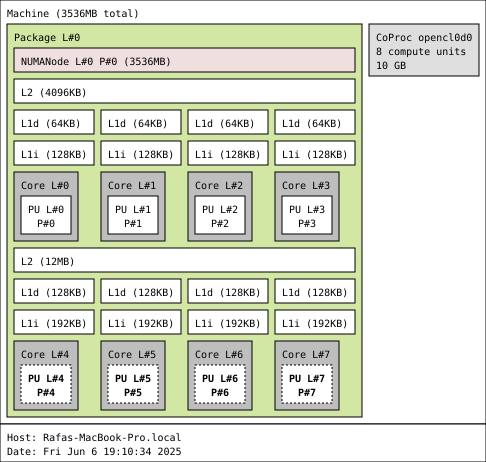
\includegraphics[width=0.8\textwidth]{images/arm.png}
\caption{Topologia procesora Apple M1 z widoczną architekturą big.LITTLE}
\label{fig:m1_topology}
\end{figure}

Platforma ARM64 reprezentowana jest przez komputer Apple MacBook Pro z następującymi specyfikacjami technicznymi:

\begin{table}[h]
\centering
\caption{Specyfikacja platformy ARM64}
\begin{tabular}{|l|l|}
\hline
\textbf{Komponent} & \textbf{Specyfikacja} \\
\hline
Procesor & Apple M1 (ARM64) \\
Architektura & 8 rdzeni (4$\times$P-core + 4$\times$E-core) \\
Pamięć podręczna L2 & 4$\times$12MB (P-cores) + 4$\times$4MB (E-cores) \\
Pamięć operacyjna & 16 GB LPDDR4X unified memory \\
System operacyjny & macOS (Darwin kernel 23.5.0) \\
Jądro systemu & \texttt{arm64} \\
Nazwa hosta & \texttt{mbp-m1} \\
\hline
\end{tabular}

\label{tab:arm64_specs}
\end{table}

Procesor Apple M1 charakteryzuje się architekturą heterogeniczną \eng{big.LITTLE} z rdzeniami o różnej wydajności:
\begin{itemize}
    \item \textbf{Performance cores (P-cores)}: 4 rdzenie wysokowydajne o częstotliwości do 3.2 GHz
    \item \textbf{Efficiency cores (E-cores)}: 4 rdzenie energooszczędne o częstotliwości do 2.0 GHz
    \item \textbf{Unified Memory Architecture}: Wspólna pamięć dla CPU i GPU eliminująca kopiowanie danych
    \item \textbf{Pamięć podręczna}: Hierarchiczna struktura z dedykowanymi poziomami L1/L2 per rdzeń
\end{itemize}

\subsubsection{Platforma x86\_64 - Intel}
\begin{figure}[H]
\centering
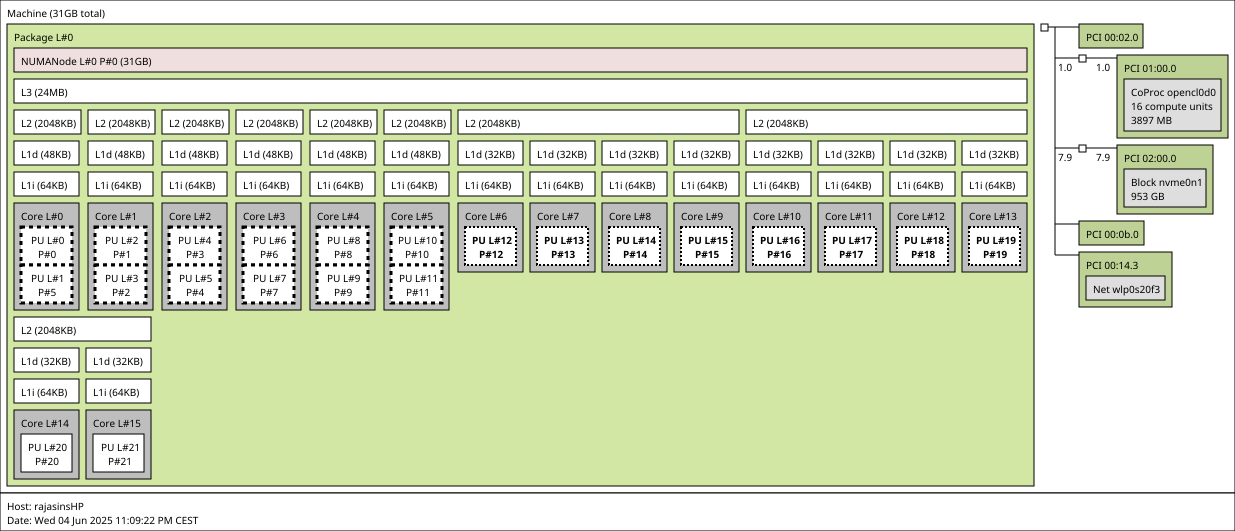
\includegraphics[width=0.8\textwidth]{images/x86.png}
\caption{Topologia procesora Intel Core Ultra 7 165H z widoczną architekturą heterogeniczną}
\label{fig:intel_topology}
\end{figure}
Platforma x86\_64 reprezentowana jest przez komputer HP z następującymi specyfikacjami technicznymi:

\begin{table}[h]
\centering
\caption{Specyfikacja platformy x86\_64}
\begin{tabular}{|l|l|}
\hline
\textbf{Komponent} & \textbf{Specyfikacja} \\
\hline
Procesor & Intel(R) Core(TM) Ultra 7 165H \\
Architektura & x86\_64 (Intel Meteor Lake) \\
Rdzenie całkowite & 22 (16 P-cores + 6 E-cores) \\
Wątki logiczne & 22 (P-cores z Hyper-Threading wyłączonym) \\
Pamięć podręczna L2 & P-cores: 2048KB $\times$ 6, E-cores: 2048KB $\times$ 8 \\
Pamięć podręczna L3 & 24MB współdzielona \\
Pamięć operacyjna & 32 GB DDR5-4800 \\
System operacyjny & Linux Ubuntu 24.04 LTS \\
Jądro systemu & 6.11.0-25-generic \\
Nazwa hosta & \texttt{hp-intel} \\
\hline
\end{tabular}

\label{tab:x86_specs}
\end{table}

Procesor Intel Core Ultra 7 165H (Meteor Lake) również wykorzystuje architekturę heterogeniczną:
\begin{itemize}
    \item \textbf{P-cores}: 6 rdzeni wysokowydajnych z obsługą Hyper-Threading (12 wątków logicznych)
    \item \textbf{E-cores}: 8 rdzeni energooszczędnych (8 wątków logicznych)
    \item \textbf{LP E-cores}: 2 rdzenie niskoenergiczne (2 wątki logiczne)
    \item \textbf{NUMA}: Non-Uniform Memory Access z Package L\#0
    \item \textbf{Technologie}: Intel Turbo Boost, Intel Speed Shift, Advanced Vector Extensions (AVX2)
\end{itemize}

\subsection{Środowiska programistyczne}

\subsubsection{Kompilatory i narzędzia}

\begin{table}[h]
\centering
\caption{Wersje kompilatorów na platformach testowych}
\begin{tabular}{|l|l|l|}
\hline
\textbf{Platforma} & \textbf{Rust} & \textbf{C++} \\
\hline
ARM64 (macOS) & rustc 1.75.0 & clang++ 14.0.3 \\
x86\_64 (Linux) & rustc 1.75.0 & g++ 11.4.0 \\
\hline
\end{tabular}

\label{tab:compilers}
\end{table}

\subsubsection{Flagi kompilacji}
\begin{itemize}
    \item \textbf{Rust}: \texttt{cargo build --release} z optymalizacjami \texttt{opt-level = 3}
    \item \textbf{C++ (Linux)}: \texttt{g++ -O3 -DNDEBUG -std=c++20 -pthread -march=native}
    \item \textbf{C++ (macOS)}: \texttt{clang++ -O3 -DNDEBUG -std=c++20 -pthread}
\end{itemize}
\subsection{Narzędzia pomiarowe i diagnostyczne}

\subsubsection{Narzędzia profilowania wydajności}

\subsubsection{Linux x86\_64 - perf}
Monitorowane metryki:
\begin{itemize}
    \item \textbf{Cykle procesora}: Całkowita liczba cykli zegara
    \item \textbf{Instrukcje}: Liczba wykonanych instrukcji
    \item \textbf{Cache performance}: Trafienia i chybienia pamięci podręcznej
    \item \textbf{Predykcja rozgałęzień}: Skuteczność branch prediction
    \item \textbf{Przełączenia kontekstu}: Częstotliwość context switching
\end{itemize}

\subsubsection{macOS ARM64 - Instruments}
Wykorzystanie pakietu Xcode Instruments:
\begin{itemize}
    \item \textbf{System Trace}: Analiza planowania wątków i synchronizacji
    \item \textbf{Allocations}: Monitorowanie alokacji i dealokacji pamięci
    \item \textbf{Time Profiler}: Profilowanie czasowe z dokładnością do funkcji
    \item \textbf{System Usage}: Wykorzystanie zasobów systemowych
\end{itemize}

\subsection{Programowanie równoległe}
W ramach programów równoległych wykorzystano jako wzorzec, gotowe implementacje problemów z zestawu NPB w ramach istniejącej pracy The NAS Parallel Benchmarks for evaluating C++ parallel programming frameworks on shared-memory architectures \cite{CPPNPB} oraz programów bazujących na nich w języku Rust, napisanych w ramach proejktu na studia przez G.Bessa et al. \cite{NPBRust}.
\subsection{Programowanie równoległe}
W ramach programów równoległych wykorzystano jako wzorzec, gotowe implementacje problemów z zestawu NPB w ramach istniejącej pracy The NAS Parallel Benchmarks for evaluating C++ parallel programming frameworks on shared-memory architectures \cite{CPPNPB} oraz programów bazujących na nich w języku Rust, napisanych w ramach proejktu na studia przez G.Bessa et al. \cite{NPBRust}.
%Porównanie Rust i C++
\chapter{Analiza wyników - programowanie równoległe}
W tym rozdziale zostały zebrane wyniki testów, które porównują ze sobą mechanizmy programowania równoległego w językach Rust i C++.

\section{Programowanie równoległe}
\subsection{OpenMP -  Open Multi-Processing}
OpenMP to biblioteka umożliwiająca programowanie równoległe w modelu pamięci współdzielonej. Jest dostępna dla języków C, C++ oraz Fortran i opiera się na użyciu dyrektyw preprocesora (ang. compiler directives) pozwalających na uproszczone rozproszenie zadań pomiędzy wątki w sposób deklaratywny.

Podstawowym celem OpenMP jest ułatwienie implementacji aplikacji równoległych poprzez maksymalne ograniczenie ręcznego zarządzania wątkami i synchronizacją. W kodzie C++ użycie tej technologii wymaga aktywacji flagi -fopenmp podczas kompilacji przy użyciu kompilatora g++.
Przedstawia podstawowe pojęcia:
\begin{itemize}
    \item \#pragma omp parallel — dyrektywa inicjująca blok kodu, który ma zostać wykonany równolegle przez wiele wątków,
    \item shared — oznacza zmienne współdzielone pomiędzy wszystkimi wątkami,
    \item private — każdemu wątkowi przypisywana jest prywatna kopia zmiennej,
    \item cache locality — pamięć podręczna (ang. cache) może znacznie poprawić wydajność przetwarzania, choć kosztem większego zużycia pamięci.
\end{itemize}

\begin{lstlisting}[language=C++, caption={Przykład użycia OpenMP w C++}, label={lst:openmp_example}]
#include <omp.h>
#include <iostream>

int main() {
    int sum = 0;
    #pragma omp parallel for reduction(+:sum)
    for (int i = 1; i <= 100; ++i) {
        sum += i;
    }
    std::cout << "Suma: " << sum << std::endl;
    return 0;
}
\end{lstlisting}    
W powyższym przykładzie w listingu \ref{lst:openmp_example} zmienna sum jest sumą liczb od 1 do 100 obliczaną równolegle. Dzięki użyciu dyrektywy \#pragma omp parallel for każda iteracja pętli może być wykonana w osobnym wątku. Atrybut reduction(+:sum) zapewnia bezpieczne sumowanie wyników lokalnych wątków do jednej wartości globalnej. OpenMP automatycznie zarządza synchronizacją i agregacją wyników, dzięki czemu użytkownik nie musi implementować ręcznego zarządzania zasobami współdzielonymi
.

\subsection{Intel TBB (Threading Building Blocks)}
Intel Threading Building Blocks (TBB) to nowoczesna biblioteka programistyczna dla języka C++, przeznaczona do tworzenia aplikacji równoległych w sposób wysoce elastyczny i skalowalny. W przeciwieństwie do OpenMP, TBB opiera się na programowaniu funkcyjnym i komponentowym, umożliwiając dekompozycję zadań \eng{ task-based parallelism}, a nie operacji niskiego poziomu.

Cechy charakterystyczne:
\begin{itemize}
    \item Deklaratywny styl programowania, który umożliwia oddelegowanie decyzji o wykonaniu do systemu planowania zadań.
    \item Dynamiczna alokacja wątków w oparciu o dostępność zasobów.
    \item Wbudowana obsługa synchronizacji oraz struktur danych przystosowanych do środowisk wielowątkowych (np. concurrent\_vector, concurrent\_queue).
\end{itemize}

\begin{lstlisting}[language=C++, caption={Przykład użycia Intel TBB w C++}, label={lst:tbb_example}]
#include <tbb/tbb.h>
#include <iostream>
#include <vector>

int main() {
    std::vector<int> data(1000, 1);
    int sum = 0;

    tbb::parallel_reduce(
        tbb::blocked_range<size_t>(0, data.size()),
        0,
        [&](const tbb::blocked_range<size_t>& r, int local_sum) {
            for (size_t i = r.begin(); i < r.end(); ++i)
                local_sum += data[i];
            return local_sum;
        },
        std::plus<int>()
    );

    std::cout << "Suma: " << sum << std::endl;
    return 0;
}
\end{lstlisting}
W powyższym przykładzie w listingu \ref{lst:tbb_example} funkcja tbb::parallel\_reduce automatycznie dzieli zakres danych na bloki (blocked\_range), które przetwarzane są równolegle przez dostępne wątki. Funkcja lambda odpowiada za lokalne przetwarzanie danych (w tym przypadku sumowanie wartości), a następnie lokalne wyniki są agregowane przy użyciu funkcji std::plus<int>. TBB samodzielnie zarządza planowaniem zadań oraz synchronizacją, co czyni go potężnym narzędziem w budowie skalowalnych aplikacji równoległych.



\chapter{Analiza wyników - programowanie współbieżne}
W tym rozdziale zostały zebrane wyniki testów, które porównują ze sobą mechanizmy progra-
mowania współbieżnego w językach Rust i C++.

\section{Programowanie współbieżne}
Współbieżność w języku C++ wspierana jest od standardu C++11, który wprowadził szereg struktur i mechanizmów umożliwiających tworzenie i synchronizację wątków. W kolejnych wersjach (C++14, C++17, C++20 i C++23) język został wzbogacony o kolejne narzędzia, zwiększające bezpieczeństwo, ekspresyjność i ergonomię programowania współbieżnego.

\subsection{Biblioteki i przestrzeń standardowa}
\subsubsection{std::thread oraz std::jthread}
Standardowa biblioteka języka C++ zawiera podstawowe komponenty do obsługi wątków w module <thread>. Wraz z C++20 wprowadzono std::jthread, będący bezpieczniejszą alternatywą dla std::thread, ponieważ automatycznie dołącza wątek w destruktorze obiektu. Dzięki temu możliwe jest uniknięcie błędów takich jak niezakończony wątek  \eng{orphaned thread} lub przedwczesne zakończenie programu.

\begin{lstlisting}[language=C++, caption={Przykład użycia std::jthread}, label={jthread_example}]
#include <iostream>
#include <thread>

void worker() {
    std::cout << "Thread is running." << std::endl;
}

int main() {
    std::jthread t(worker); // wątek zarządzany automatycznie
    // brak konieczności wywoływania join() lub detach()
}
\end{lstlisting}    
W przykładzie listing \ref{jthread_example} utworzono nowy wątek wątek z użyciem std::jthread, który uruchamia funkcję worker. Dzięki automatycznemu zarządzaniu zasobami przez std::jthread, nie ma potrzeby ręcznego wywoływania join(), co zmniejsza ryzyko błędów synchronizacji.


\subsection{Komunikacja między wątkami}
C++ nie posiada wbudowanych kanałów \eng{channels} występujących w języku Rust, lecz umożliwia komunikację poprzez konstrukcje takie jak: kolejki, zmienne warunkowe (std::condition\_variable) oraz typy atomowe (std::atomic). Jednym z najczęstszych wzorców komunikacyjnych jest użycie kolejki chronionej mutexem oraz sygnalizowanej zmienną warunkową.
\begin{lstlisting}[language=C++, caption={Przykład komunikacji między wątkami}, label={condition_variable_example}]
#include <iostream>
#include <thread>
#include <queue>
#include <mutex>
#include <condition_variable>

std::queue<int> buffer;
std::mutex mtx;
std::condition_variable cv;

void producer() {
    std::unique_lock<std::mutex> lock(mtx);
    buffer.push(100); // produkcja danych
    cv.notify_one();  // powiadom konsumenta
}

void consumer() {
    std::unique_lock<std::mutex> lock(mtx);
    cv.wait(lock, [] { return !buffer.empty(); }); // czekaj na dane
    std::cout << "Consumed: " << buffer.front() << std::endl;
    buffer.pop(); // usuń dane z kolejki
}
\end{lstlisting}
Powyższy przykład listing \ref{condition_variable_example} implementuje prosty scenariusz producent-konsument. Producent wstawia dane do kolejki i powiadamia wątek oczekujący. Konsument blokuje się, dopóki kolejka nie będzie zawierać danych. Zmienna warunkowa eliminuje konieczność aktywnego sprawdzania warunku (busy waiting), co poprawia efektywność systemu.


\subsection{Synchronizacja}
Synchronizacja w języku C++ opiera się głównie na mutexach (std::mutex) oraz ich odmianach. Od C++17 dostępny jest std::scoped\_lock, pozwalający na bezpieczne blokowanie wielu mutexów jednocześnie, a od C++20 wprowadzono bardziej zaawansowane konstrukty takie jak std::latch i std::barrier, które umożliwiają synchronizację wielu wątków na określonym etapie wykonania.

\begin{lstlisting}[language=C++, caption={Przykład użycia std::scoped\_lock}, label={scoped_lock_example}]
#include <iostream>
#include <thread>
#include <mutex>

int counter = 0;
std::mutex mtx;

void increment() {
    std::lock_guard<std::mutex> lock(mtx); // automatyczna blokada mutexu
    ++counter;
}

int main() {
    std::thread t1(increment);
    std::thread t2(increment);
    t1.join();
    t2.join();
    std::cout << "Counter: " << counter << std::endl;
}
\end{lstlisting}
W tym przykładzie - listing \ref{scoped_lock_example} dwa wątki próbują jednocześnie zwiększyć wartość zmiennej counter. Aby zapobiec wyścigowi danych, dostęp do zasobu jest chroniony przez std::mutex. Użycie std::lock\_guard zapewnia, że blokada zostanie zwolniona automatycznie po wyjściu z zakresu funkcji.

\subsubsection{std::latch oraz std::barrier (C++20)}
Mechanizmy std::latch oraz std::barrier wprowadzone w standardzie C++20 służą do synchronizacji wielu wątków w określonym punkcie programu:
\begin{itemize}
    \item std::latch - jednorazowy licznik synchronizacyjny, który pozwala wątkom oczekującym na rozpoczęcie działania, aż inne wątki zakończą przygotowanie.
    \item std::barrier - wielokrotnego użytku, synchronizuje grupę wątków po osiągnięciu „cyklu bariery”.
\end{itemize}
\begin{lstlisting}[language=C++, caption={Przykład użycia std::latch oraz std::barrier}, label={latch_barrier_example}]
#include <iostream>
#include <thread>
#include <latch>
#include <barrier>

constexpr int num_threads = 3;
std::latch start_latch(num_threads);
std::barrier sync_barrier(num_threads);

void worker(int id) {
    std::cout << "Thread " << id << " is initializing.\n";
    start_latch.arrive_and_wait(); // czekaj aż wszystkie wątki się przygotują
    for (int i = 0; i < 2; ++i) {
        std::cout << "Thread " << id << " is processing iteration " << i << ".\n";

        // Synchronizacja między iteracjami
        sync_barrier.arrive_and_wait();

        std::cout << "Thread " << id << " passed the barrier in iteration " << i << ".\n";
    }
}
int main() {
    std::thread threads[num_threads];
    for (int i = 0; i < num_threads; ++i)
    threads[i] = std::thread(worker, i + 1);
    for (auto& t : threads)
        t.join();
}
\end{lstlisting}    
W listingu \ref{latch_barrier_example} każdy wątek najpierw dochodzi do punktu synchronizacji std::latch, oczekując aż wszystkie inne wątki również zakończą fazę inicjalizacji. Następnie, w dwóch kolejnych iteracjach przetwarzania danych, zastosowany zostaje std::barrier, który gwarantuje, że wszystkie wątki ukończą daną iterację przed przejściem do kolejnej. Takie podejście zwiększa spójność przetwarzania i eliminuje potencjalne niespójności wynikające z wyścigów czasowych między wątkami.

\subsection{Asynchroniczność}
Programowanie asynchroniczne w C++ możliwe jest dzięki konstrukcjom takim jak std::async, std::future i std::promise. std::async uruchamia funkcję w tle i umożliwia jej obserwację za pomocą obiektu future. Podejście to ułatwia uruchamianie zadań bez konieczności jawnego zarządzania wątkiem.

\begin{lstlisting}[language=C++, caption={Przykład użycia std::async}, label={async_example}]
    #include <iostream>
    #include <future>
    
    int compute() {
        return 2 * 21;
    }
    
    int main() {
        std::future<int> result = std::async(std::launch::async, compute);
        std::cout << "Result: " << result.get() << std::endl;
    }
\end{lstlisting}
W powyższym listingu \ref{async_example} funkcja compute() zostaje uruchomiona asynchronicznie. std::future pozwala na uzyskanie wyniku, gdy ten będzie dostępny. W ten sposób możemy kontynuować inne działania, a wynik odebrać w późniejszym czasie — co jest przydatne w aplikacjach wymagających wysokiej responsywności.

\subsubsection{std::promise}
Obiekt std::promise (obietnica) w języku C++ umożliwia przekazywanie wartości z jednego wątku do drugiego. Stanowi uzupełnienie mechanizmu std::future, ponieważ pozwala manualnie ustawić wartość, którą future później odbierze. Dzięki temu rozdzielona zostaje produkcja i konsumpcja danych między wątkami, umożliwiając bardziej elastyczne projektowanie asynchronicznych przepływów sterowania.
\begin{lstlisting}[language=C++, caption={Przykład użycia std::promise}, label={promise_example}]
#include <iostream>
#include <thread>
#include <future>

// Funkcja symulująca kosztowne obliczenie
int compute(int x) {
    return x * 2;
}

int main() {
    std::promise<int> promise; // utworzenie obiektu obietnicy
    std::future<int> result = promise.get_future(); // pobranie powiązanego future

    std::thread producer([&promise]() {
        int value = 21;
        int result = compute(value);
        promise.set_value(result); // ustawienie wartości, która zostanie odebrana przez future
    });

    std::cout << "Result: " << result.get() << std::endl; // odbiór wartości, blokuje do czasu jej ustawienia
    producer.join();

    return 0;
}
\end{lstlisting}    
W listingu \ref{promise_example} wątek główny tworzy promise i pobiera powiązany z nim future. Wątek producer wykonuje obliczenie i przekazuje wynik przez promise. Funkcja result.get() wstrzymuje główny wątek do czasu dostępności wyniku.
\subsubsection{std::packaged\_task}
std::packaged\_task to obiekt otaczający dowolną wywoływalną funkcję (np. funkcję, lambda, std::bind), który integruje się z future. Pozwala to uruchomić zadanie w wątku i obserwować jego wynik.
\begin{lstlisting}[language=C++, caption={Przykład użycia std::packaged\_task}, label={packaged_task_example}]
#include <iostream>
#include <thread>
#include <future>

// Funkcja do opakowania w packaged_task
int compute(int x) {
    return x * 2;
}

int main() {
    std::packaged_task<int(int)> task(compute); // utworzenie zapakowanego zadania
    std::future<int> result = task.get_future(); // pobranie powiązanego future

    std::thread worker(std::move(task), 21); // uruchomienie zadania w wątku z parametrem 21

    std::cout << "Result: " << result.get() << std::endl; // odbiór wyniku
    worker.join();

    return 0;
}
\end{lstlisting}
W powyższym przykładzie listing \ref{packaged_task_example} funkcja compute została opakowana w packaged\_task, a następnie uruchomiona w osobnym wątku z argumentem 21. Wynik trafia do future, który umożliwia jego odbiór w wątku głównym. przetwarzanie zadań.

\subsubsection{C++23 - std::task i std::execution}
Standard C++23 (najnowszy w chwili tworzenia niniejszej pracy) wprowadza nowe pojęcia:
\begin{itemize}
    \item std::task - reprezentuje zadanie, które można uruchomić z użyciem określonego planisty wykonania.
    \item std::execution - zestaw polityk (strategii) określających sposób wykonywania zadań, takich jak sekwencyjnie, współbieżnie, równolegle.
\end{itemize}

Mechanizmy te są częścią trwającej transformacji C++ w kierunku deklaratywnego modelu programowania współbieżnego i równoległego. Mają one zostać wprowadzone wstępnie w wersji C++26 \cite{cpp26} Ponieważ wsparcie dla tych mechanizmów jest na etapie wdrażania, nie będą one szczegółowo omawiane w tej pracy. Warto jednak zauważyć, że ich celem jest uproszczenie i ujednolicenie podejścia do programowania współbieżnego, podobnie jak ma to miejsce w języku Rust.
%Porównanie Rust i C++
\chapter{Analiza wyników - programowanie równoległe}
W tym rozdziale zostały zebrane wyniki testów, które porównują ze sobą mechanizmy programowania równoległego w językach Rust i C++.
\nopagebreak
\section{Programowanie równoległe}
\subsection{OpenMP -  Open Multi-Processing}
OpenMP to biblioteka umożliwiająca programowanie równoległe w modelu pamięci współdzielonej. Jest dostępna dla języków C, C++ oraz Fortran i opiera się na użyciu dyrektyw preprocesora (ang. compiler directives) pozwalających na uproszczone rozproszenie zadań pomiędzy wątki w sposób deklaratywny.

Podstawowym celem OpenMP jest ułatwienie implementacji aplikacji równoległych poprzez maksymalne ograniczenie ręcznego zarządzania wątkami i synchronizacją. W kodzie C++ użycie tej technologii wymaga aktywacji flagi -fopenmp podczas kompilacji przy użyciu kompilatora g++.
Przedstawia podstawowe pojęcia:
\begin{itemize}
    \item \#pragma omp parallel — dyrektywa inicjująca blok kodu, który ma zostać wykonany równolegle przez wiele wątków,
    \item shared — oznacza zmienne współdzielone pomiędzy wszystkimi wątkami,
    \item private — każdemu wątkowi przypisywana jest prywatna kopia zmiennej,
    \item cache locality — pamięć podręczna (ang. cache) może znacznie poprawić wydajność przetwarzania, choć kosztem większego zużycia pamięci.
\end{itemize}

\begin{lstlisting}[language=C++, caption={Przykład użycia OpenMP w C++}, label={lst:openmp_example}]
#include <omp.h>
#include <iostream>

int main() {
    int sum = 0;
    #pragma omp parallel for reduction(+:sum)
    for (int i = 1; i <= 100; ++i) {
        sum += i;
    }
    std::cout << "Suma: " << sum << std::endl;
    return 0;
}
\end{lstlisting}    
W powyższym przykładzie w listingu \ref{lst:openmp_example} zmienna sum jest sumą liczb od 1 do 100 obliczaną równolegle. Dzięki użyciu dyrektywy \#pragma omp parallel for każda iteracja pętli może być wykonana w osobnym wątku. Atrybut reduction(+:sum) zapewnia bezpieczne sumowanie wyników lokalnych wątków do jednej wartości globalnej. OpenMP automatycznie zarządza synchronizacją i agregacją wyników, dzięki czemu użytkownik nie musi implementować ręcznego zarządzania zasobami współdzielonymi
.

\subsection{Intel TBB (Threading Building Blocks)}
Intel Threading Building Blocks (TBB) to nowoczesna biblioteka programistyczna dla języka C++, przeznaczona do tworzenia aplikacji równoległych w sposób wysoce elastyczny i skalowalny. W przeciwieństwie do OpenMP, TBB opiera się na programowaniu funkcyjnym i komponentowym, umożliwiając dekompozycję zadań \eng{ task-based parallelism}, a nie operacji niskiego poziomu.

Cechy charakterystyczne:
\begin{itemize}
    \item Deklaratywny styl programowania, który umożliwia oddelegowanie decyzji o wykonaniu do systemu planowania zadań.
    \item Dynamiczna alokacja wątków w oparciu o dostępność zasobów.
    \item Wbudowana obsługa synchronizacji oraz struktur danych przystosowanych do środowisk wielowątkowych (np. concurrent\_vector, concurrent\_queue).
\end{itemize}

\begin{lstlisting}[language=C++, caption={Przykład użycia Intel TBB w C++}, label={lst:tbb_example}]
#include <tbb/tbb.h>
#include <iostream>
#include <vector>

int main() {
    std::vector<int> data(1000, 1);
    int sum = 0;

    tbb::parallel_reduce(
        tbb::blocked_range<size_t>(0, data.size()),
        0,
        [&](const tbb::blocked_range<size_t>& r, int local_sum) {
            for (size_t i = r.begin(); i < r.end(); ++i)
                local_sum += data[i];
            return local_sum;
        },
        std::plus<int>()
    );

    std::cout << "Suma: " << sum << std::endl;
    return 0;
}
\end{lstlisting}
W powyższym przykładzie w listingu \ref{lst:tbb_example} funkcja tbb::parallel\_reduce automatycznie dzieli zakres danych na bloki (blocked\_range), które przetwarzane są równolegle przez dostępne wątki. Funkcja lambda odpowiada za lokalne przetwarzanie danych (w tym przypadku sumowanie wartości), a następnie lokalne wyniki są agregowane przy użyciu funkcji std::plus<int>. TBB samodzielnie zarządza planowaniem zadań oraz synchronizacją, co czyni go potężnym narzędziem w budowie skalowalnych aplikacji równoległych.



% \chapter{Analiza wyników - programowanie współbieżne}
W tym rozdziale zostały zebrane wyniki testów, które porównują ze sobą mechanizmy progra-
mowania współbieżnego w językach Rust i C++.

\section{Programowanie współbieżne}
Współbieżność w języku C++ wspierana jest od standardu C++11, który wprowadził szereg struktur i mechanizmów umożliwiających tworzenie i synchronizację wątków. W kolejnych wersjach (C++14, C++17, C++20 i C++23) język został wzbogacony o kolejne narzędzia, zwiększające bezpieczeństwo, ekspresyjność i ergonomię programowania współbieżnego.

\subsection{Biblioteki i przestrzeń standardowa}
\subsubsection{std::thread oraz std::jthread}
Standardowa biblioteka języka C++ zawiera podstawowe komponenty do obsługi wątków w module <thread>. Wraz z C++20 wprowadzono std::jthread, będący bezpieczniejszą alternatywą dla std::thread, ponieważ automatycznie dołącza wątek w destruktorze obiektu. Dzięki temu możliwe jest uniknięcie błędów takich jak niezakończony wątek  \eng{orphaned thread} lub przedwczesne zakończenie programu.

\begin{lstlisting}[language=C++, caption={Przykład użycia std::jthread}, label={jthread_example}]
#include <iostream>
#include <thread>

void worker() {
    std::cout << "Thread is running." << std::endl;
}

int main() {
    std::jthread t(worker); // wątek zarządzany automatycznie
    // brak konieczności wywoływania join() lub detach()
}
\end{lstlisting}    
W przykładzie listing \ref{jthread_example} utworzono nowy wątek wątek z użyciem std::jthread, który uruchamia funkcję worker. Dzięki automatycznemu zarządzaniu zasobami przez std::jthread, nie ma potrzeby ręcznego wywoływania join(), co zmniejsza ryzyko błędów synchronizacji.


\subsection{Komunikacja między wątkami}
C++ nie posiada wbudowanych kanałów \eng{channels} występujących w języku Rust, lecz umożliwia komunikację poprzez konstrukcje takie jak: kolejki, zmienne warunkowe (std::condition\_variable) oraz typy atomowe (std::atomic). Jednym z najczęstszych wzorców komunikacyjnych jest użycie kolejki chronionej mutexem oraz sygnalizowanej zmienną warunkową.
\begin{lstlisting}[language=C++, caption={Przykład komunikacji między wątkami}, label={condition_variable_example}]
#include <iostream>
#include <thread>
#include <queue>
#include <mutex>
#include <condition_variable>

std::queue<int> buffer;
std::mutex mtx;
std::condition_variable cv;

void producer() {
    std::unique_lock<std::mutex> lock(mtx);
    buffer.push(100); // produkcja danych
    cv.notify_one();  // powiadom konsumenta
}

void consumer() {
    std::unique_lock<std::mutex> lock(mtx);
    cv.wait(lock, [] { return !buffer.empty(); }); // czekaj na dane
    std::cout << "Consumed: " << buffer.front() << std::endl;
    buffer.pop(); // usuń dane z kolejki
}
\end{lstlisting}
Powyższy przykład listing \ref{condition_variable_example} implementuje prosty scenariusz producent-konsument. Producent wstawia dane do kolejki i powiadamia wątek oczekujący. Konsument blokuje się, dopóki kolejka nie będzie zawierać danych. Zmienna warunkowa eliminuje konieczność aktywnego sprawdzania warunku (busy waiting), co poprawia efektywność systemu.


\subsection{Synchronizacja}
Synchronizacja w języku C++ opiera się głównie na mutexach (std::mutex) oraz ich odmianach. Od C++17 dostępny jest std::scoped\_lock, pozwalający na bezpieczne blokowanie wielu mutexów jednocześnie, a od C++20 wprowadzono bardziej zaawansowane konstrukty takie jak std::latch i std::barrier, które umożliwiają synchronizację wielu wątków na określonym etapie wykonania.

\begin{lstlisting}[language=C++, caption={Przykład użycia std::scoped\_lock}, label={scoped_lock_example}]
#include <iostream>
#include <thread>
#include <mutex>

int counter = 0;
std::mutex mtx;

void increment() {
    std::lock_guard<std::mutex> lock(mtx); // automatyczna blokada mutexu
    ++counter;
}

int main() {
    std::thread t1(increment);
    std::thread t2(increment);
    t1.join();
    t2.join();
    std::cout << "Counter: " << counter << std::endl;
}
\end{lstlisting}
W tym przykładzie - listing \ref{scoped_lock_example} dwa wątki próbują jednocześnie zwiększyć wartość zmiennej counter. Aby zapobiec wyścigowi danych, dostęp do zasobu jest chroniony przez std::mutex. Użycie std::lock\_guard zapewnia, że blokada zostanie zwolniona automatycznie po wyjściu z zakresu funkcji.

\subsubsection{std::latch oraz std::barrier (C++20)}
Mechanizmy std::latch oraz std::barrier wprowadzone w standardzie C++20 służą do synchronizacji wielu wątków w określonym punkcie programu:
\begin{itemize}
    \item std::latch - jednorazowy licznik synchronizacyjny, który pozwala wątkom oczekującym na rozpoczęcie działania, aż inne wątki zakończą przygotowanie.
    \item std::barrier - wielokrotnego użytku, synchronizuje grupę wątków po osiągnięciu „cyklu bariery”.
\end{itemize}
\begin{lstlisting}[language=C++, caption={Przykład użycia std::latch oraz std::barrier}, label={latch_barrier_example}]
#include <iostream>
#include <thread>
#include <latch>
#include <barrier>

constexpr int num_threads = 3;
std::latch start_latch(num_threads);
std::barrier sync_barrier(num_threads);

void worker(int id) {
    std::cout << "Thread " << id << " is initializing.\n";
    start_latch.arrive_and_wait(); // czekaj aż wszystkie wątki się przygotują
    for (int i = 0; i < 2; ++i) {
        std::cout << "Thread " << id << " is processing iteration " << i << ".\n";

        // Synchronizacja między iteracjami
        sync_barrier.arrive_and_wait();

        std::cout << "Thread " << id << " passed the barrier in iteration " << i << ".\n";
    }
}
int main() {
    std::thread threads[num_threads];
    for (int i = 0; i < num_threads; ++i)
    threads[i] = std::thread(worker, i + 1);
    for (auto& t : threads)
        t.join();
}
\end{lstlisting}    
W listingu \ref{latch_barrier_example} każdy wątek najpierw dochodzi do punktu synchronizacji std::latch, oczekując aż wszystkie inne wątki również zakończą fazę inicjalizacji. Następnie, w dwóch kolejnych iteracjach przetwarzania danych, zastosowany zostaje std::barrier, który gwarantuje, że wszystkie wątki ukończą daną iterację przed przejściem do kolejnej. Takie podejście zwiększa spójność przetwarzania i eliminuje potencjalne niespójności wynikające z wyścigów czasowych między wątkami.

\subsection{Asynchroniczność}
Programowanie asynchroniczne w C++ możliwe jest dzięki konstrukcjom takim jak std::async, std::future i std::promise. std::async uruchamia funkcję w tle i umożliwia jej obserwację za pomocą obiektu future. Podejście to ułatwia uruchamianie zadań bez konieczności jawnego zarządzania wątkiem.

\begin{lstlisting}[language=C++, caption={Przykład użycia std::async}, label={async_example}]
    #include <iostream>
    #include <future>
    
    int compute() {
        return 2 * 21;
    }
    
    int main() {
        std::future<int> result = std::async(std::launch::async, compute);
        std::cout << "Result: " << result.get() << std::endl;
    }
\end{lstlisting}
W powyższym listingu \ref{async_example} funkcja compute() zostaje uruchomiona asynchronicznie. std::future pozwala na uzyskanie wyniku, gdy ten będzie dostępny. W ten sposób możemy kontynuować inne działania, a wynik odebrać w późniejszym czasie — co jest przydatne w aplikacjach wymagających wysokiej responsywności.

\subsubsection{std::promise}
Obiekt std::promise (obietnica) w języku C++ umożliwia przekazywanie wartości z jednego wątku do drugiego. Stanowi uzupełnienie mechanizmu std::future, ponieważ pozwala manualnie ustawić wartość, którą future później odbierze. Dzięki temu rozdzielona zostaje produkcja i konsumpcja danych między wątkami, umożliwiając bardziej elastyczne projektowanie asynchronicznych przepływów sterowania.
\begin{lstlisting}[language=C++, caption={Przykład użycia std::promise}, label={promise_example}]
#include <iostream>
#include <thread>
#include <future>

// Funkcja symulująca kosztowne obliczenie
int compute(int x) {
    return x * 2;
}

int main() {
    std::promise<int> promise; // utworzenie obiektu obietnicy
    std::future<int> result = promise.get_future(); // pobranie powiązanego future

    std::thread producer([&promise]() {
        int value = 21;
        int result = compute(value);
        promise.set_value(result); // ustawienie wartości, która zostanie odebrana przez future
    });

    std::cout << "Result: " << result.get() << std::endl; // odbiór wartości, blokuje do czasu jej ustawienia
    producer.join();

    return 0;
}
\end{lstlisting}    
W listingu \ref{promise_example} wątek główny tworzy promise i pobiera powiązany z nim future. Wątek producer wykonuje obliczenie i przekazuje wynik przez promise. Funkcja result.get() wstrzymuje główny wątek do czasu dostępności wyniku.
\subsubsection{std::packaged\_task}
std::packaged\_task to obiekt otaczający dowolną wywoływalną funkcję (np. funkcję, lambda, std::bind), który integruje się z future. Pozwala to uruchomić zadanie w wątku i obserwować jego wynik.
\begin{lstlisting}[language=C++, caption={Przykład użycia std::packaged\_task}, label={packaged_task_example}]
#include <iostream>
#include <thread>
#include <future>

// Funkcja do opakowania w packaged_task
int compute(int x) {
    return x * 2;
}

int main() {
    std::packaged_task<int(int)> task(compute); // utworzenie zapakowanego zadania
    std::future<int> result = task.get_future(); // pobranie powiązanego future

    std::thread worker(std::move(task), 21); // uruchomienie zadania w wątku z parametrem 21

    std::cout << "Result: " << result.get() << std::endl; // odbiór wyniku
    worker.join();

    return 0;
}
\end{lstlisting}
W powyższym przykładzie listing \ref{packaged_task_example} funkcja compute została opakowana w packaged\_task, a następnie uruchomiona w osobnym wątku z argumentem 21. Wynik trafia do future, który umożliwia jego odbiór w wątku głównym. przetwarzanie zadań.

\subsubsection{C++23 - std::task i std::execution}
Standard C++23 (najnowszy w chwili tworzenia niniejszej pracy) wprowadza nowe pojęcia:
\begin{itemize}
    \item std::task - reprezentuje zadanie, które można uruchomić z użyciem określonego planisty wykonania.
    \item std::execution - zestaw polityk (strategii) określających sposób wykonywania zadań, takich jak sekwencyjnie, współbieżnie, równolegle.
\end{itemize}

Mechanizmy te są częścią trwającej transformacji C++ w kierunku deklaratywnego modelu programowania współbieżnego i równoległego. Mają one zostać wprowadzone wstępnie w wersji C++26 \cite{cpp26} Ponieważ wsparcie dla tych mechanizmów jest na etapie wdrażania, nie będą one szczegółowo omawiane w tej pracy. Warto jednak zauważyć, że ich celem jest uproszczenie i ujednolicenie podejścia do programowania współbieżnego, podobnie jak ma to miejsce w języku Rust.



% SPIS RYSUNKÓW (zostanie wygenerowany automatycznie)
\pdfbookmark[0]{Spis rysunków}{spisRysunkow.1} % jeśli chcemy mieć w spisie treści, to zamarkować tę linię, a odmarkować linie poniższe
\phantomsection
\addcontentsline{toc}{chapter}{Spis rysunków}
\listoffigures*
\clearpage

% SPIS TABEL (zostanie wygenerowany automatycznie)
\pdfbookmark[0]{Spis tabel}{spisTabel.1} %
\phantomsection
\addcontentsline{toc}{chapter}{Spis tabel}
\listoftables*
\clearpage

% SPIS LISTINGÓW (zostanie wygenerowany automatycznie)
\pdfbookmark[0]{Spis listingów}{spisListingow.1} %
\phantomsection
\addcontentsline{toc}{chapter}{Spis listingów}
\lstlistoflistings*

% LITERATURA (zostanie wygenerowana automatycznie)
%UWAGA: bibliotekę referencji należy przygotować samemu. Dobrym do tego narzędziem jest JabRef.
%       JabRef oferuje jednak większą liczbę typów rekordów niż obsługuje BibTeX.
%       Proszę nie deklarować rekordów o typach nieobsługiwanych przez BibTeX.
%       Formatowania wykazu literatury i cytowań odbywać się ma zgodnie z zadeklarowanym stylem.
%       Zalecane są style produkujące numeryczne cytowania (w postaci [1], [2,3]).
%       Takim stylem jest np. plabbrv
\bibliographystyle{plabbrv}
%       Aby zapanować nad odstępami w wykazie literatury można posłużyć się poniższą komendą
\setlength{\bibitemsep}{2pt} % - zacieśnia wykaz
%       Pozycja Literatura pojawia się w spisie treści nieco inaczej niż spisy rysunków, tabel itp.
%       Aby zachować właściwe odstępy należy użyć poniższej komendy
\addtocontents{toc}{\addvspace{2pt}} % ustawiamy odstęp w spisie treści przed pozycją Literatura 
%       Nazwę pliku przygotowanej biblioteki wpisuje się bez rozszerzenia .bib
%       (linia poniżej załaduje rekordy z pliku "dokumentacja.bib")
\bibliography{dokumentacja}
\nocite{*}

\appendix
%\chapter{Instrukcja wdrożeniowa}
Jeśli praca kończy się tworzeniem oprogramowania, to w dodatku powinna znaleźć się instrukcja wdrożeniowa, która opisuje, jak skompilować lub zainstalować to oprogramowanie.

Dodatkowo, przyda się krótka instrukcja ,,how to'' (jak uruchomić system i wykonać podstawową czynność). Można to zaprezentować na prostym przypadku użycia. Warto rozważyć umieszczenie tych informacji w osobnym dodatku.

%\chapter{Opis załączonej płyty CD/DVD}
\label{chap:opis-plyty}
Ten rozdział jest miejscem, w którym zamieszczamy opis zawartości dołączonej płyty. Należy pamiętać, że opis ten jest przygotowywany przed załadowaniem pracy do systemu APD USOS, dlatego nie znamy jeszcze nazwy, jaką ten system wygeneruje dla załadowanego pliku. Dlatego warto stosować ogólniki typu: "Na płycie zamieszczono dokument PDF z tekstem pracy" bez wskazywania nazwy konkretnego pliku.

Wcześniej obowiązywała reguła, aby nadawać dokumentom nazwy zgodnie z wzorcem "W04\_[numer albumu]\_[rok kalendarzowy]\_[rodzaj pracy]". Rok kalendarzowy odnosił się do roku realizacji kursu "Praca dyplomowa", a nie roku obrony. Na przykład, wzorzec nazwy dla pracy dyplomowej inżynierskiej wyglądałby tak: "W04\_123456\_2015\_praca inżynierska.pdf". Takie nazwy były utrwalane w systemie składania prac dyplomowych. Jednak obecnie procedura jest inna.


% Jeśli w pracy pojawiać się ma indeks, należy odkomentować poniższe linie
%%\chapterstyle{noNumbered}
%%\phantomsection % sets an anchor
%%\addcontentsline{toc}{chapter}{Indeks rzeczowy}
%%\printindex

\end{document}
